\documentclass[12pt]{article}

\usepackage{geometry}
\usepackage{amsfonts}
\usepackage{amssymb}
\usepackage{amsmath}
\usepackage{fancyhdr}
\usepackage{unicode-math}
\usepackage{titlesec}
\usepackage{enumitem}
\usepackage{graphicx}
\usepackage{wrapfig}
\usepackage[labelfont=bf, skip=5pt]{caption}
\usepackage{setspace}
\usepackage{hyperref}
\usepackage{booktabs}
\usepackage{cleveref}
\usepackage[square, numbers]{natbib}
\usepackage{doi}
\usepackage[nottoc, numbib]{tocbibind}
\usepackage{minted}

\newcommand{\brackets}[1]{\left[\,#1\,\right]}
\newcommand{\paren}[1]{\left( #1 \right)}
\newcommand{\curls}[1]{\left\{#1\right\}}
\newcommand{\verts}[1]{\left\lvert #1 \right\rvert}
\newcommand{\angled}[1]{\left\langle #1 \right\rangle}
\newcommand{\ket}[1]{\left\lvert #1 \right\rangle}
\newcommand{\bra}[1]{\left\langle #1 \right\rvert}

\bibliographystyle{unsrtnat}
% new environment for listings (code) that can span over multiple pages
\newenvironment{code}{\captionsetup{type=listing}}{\par\addvspace{\baselineskip}}
\renewcommand{\thefootnote}{\alph{footnote}}
% vertical space above & below [h] floats
\setlength{\intextsep}{5pt}
% Alternative style section
\titleformat{\section}[block]{\normalfont\itshape}{\thesection}{0.5em}{\titlerule\\[.8ex]\bfseries}

\geometry{b4paper, top=2cm, left=2.5cm, right=2.5cm, bottom=2cm}
\setlist{nosep, leftmargin=\parindent}

\begin{document}\sloppy % tex.stackexchange.com/questions/9107/

\pagenumbering{roman}
\begin{titlepage}
    \begin{center}
        \vspace*{0.8cm}

        
\includegraphics[page=1,width=5cm]{img/ucl.pdf}
        \vspace{0.5cm}

        \Huge\textbf{Creation of a Graphical User Interface for the Analysis of Quantum Dynamics Simulations}
        \vspace{1.5cm}
        
        \LARGE Wenzhao Jia
        
        \vfill
        
        A dissertation presented for the degree of\\
        \textbf{Master of Science}\\
        of\\
        \textbf{University College London}
        
        \vspace{0.8cm}
        
        \Large
        Scientific and Data Intensive Computing\\
        Department of Physics and Astronomy\\
        September 2023
    \end{center}
\end{titlepage}

\setcounter{page}{2}
\subsection*{Abstract}
The \textit{Quantics} package is a set of programs for quantum dynamics simulations that solves the time-dependent Schr\"odinger equation for a set of initial conditions defined by the user via input files. The propagated wavefunction, as well as other details from the calculation, can then be analysed using \textit{Quantics}' analysis programs, a library of approximately 60 standalone executables that are called on a command line interface (CLI). The aim of this dissertation is to detail to development of a graphical user interface (GUI) which bundles the most important analysis programs together into one program coupled with a user-friendly interface that allows the user to select, execute, and visualise analysis programs without the cumbersome and manual use of a CLI, as well as to produce a solid framework such that integration with future analysis programs are as easy as possible.

\subsection*{Disclaimer}
I, Wenzhao Jia, confirm that the work presented in this dissertation is my own. Where information has been derived from other sources, I confirm that this has been indicated in the dissertation.
\vspace{0.5cm}
\newline The accompanying code for this dissertation can be found in the \texttt{analysis\_gui} branch of the \textit{Quantics} GitLab repository, available at \url{https://gitlab.com/quantics/quantics/-/tree/analysis_gui}. Access to the repository is granted on request by contacting Graham Worth at \href{mailto:g.a.worth@ucl.ac.uk}{\texttt{g.a.worth@ucl.ac.uk}}.

\subsection*{Acknowledgements}

For supervision over this project, I would like to thank Graham Worth and especially Michael Parkes for the weekly meetings which helped encourage me to keep me on track by allowing me to report new implementations in the code to him every week. His support during the write-up of the dissertation was also greatly appreciated. Overall, the dissertation ended up with almost 30,000 words; for comparison the recommended word count around 8,000. I definitely overextended with the project!
\vspace{0.5cm}
\newline Secondly, I would like to give my thanks to programme tutor Stephen Fossey and academic advisor Joseph Frost-Schenk for staying in touch with me over the late summer period through email. Finally, I must thank my parents, grandparents, and our two family cats who have been present alongside me through some dark times.

\vspace{2.5cm}

\begin{figure}[h]
    \centering
    \begin{minipage}[]{.45\textwidth}
        \centering
        
\includegraphics[width=0.5\textwidth]{img/murphy.jpg}
        \caption*{\textit{Murphy}.}
    \end{minipage}\hfill\begin{minipage}[]{.45\textwidth}
        \centering
        
\includegraphics[width=0.5\textwidth]{img/domino.jpg}
        \caption*{\textit{Domino}.}
    \end{minipage}
\end{figure}

\pagebreak
\tableofcontents

\pagebreak
\pagenumbering{arabic}
\section{Introduction}\label{sec:intro}

\subsection{The Quantics package}\label{ssec:quantics}

Molecular quantum dynamics deals with the behaviour of molecular systems. Such behaviour consists of the motion of nuclei and electrons, whose properties are governed by quantum mechanics. The realm of quantum mechanics give rise to various chemical and physical phenomena such as molecular interactions, electron scattering, and bond breaking, which can be studied via the movement of these particles.\textsuperscript{\cite{molquandym}}

These phenomena occur at the \textit{femtosecond} time scale. The field of study around this time-scale is called \textit{femtochemistry},\textsuperscript{\cite{femtochemistry}} and experiments that operate at the atomic and ultra-fast level require accompanying calculations to obtain a molecular interpretation. These calculations can be performed by quantum dynamics simulations.

The \textit{Quantics} package is a suite of programs dedicated to such a task.\textsuperscript{\cite{quantics}} By solving the time-dependent Schr\"odinger equation, the time-evolution of the molecular system can be examined, and complete information on quantum effects can be observed. The origins of the \textit{Quantics} package stem from when Uwe Manthe, as part of his PhD, created the initial code\textsuperscript{\cite{mctdh1990}} in Fortran, which is the primary programming language used for the package to this day.\textsuperscript{\cite{quanticsreview}}

\begin{figure}[h]
    \centering
    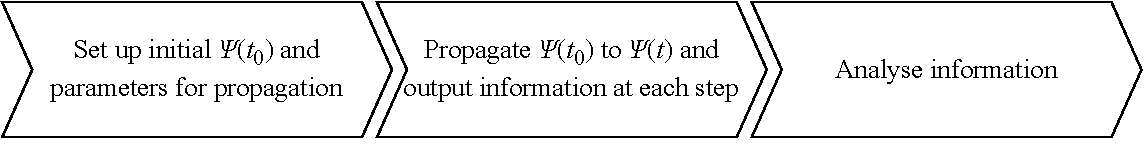
\includegraphics[page=1,width=0.8\textwidth]{img/sim_steps.pdf}
    \caption{The three underlying processes of a quantum dynamics simulation. \(\symit{Ψ}\) is the wavefunction, which describes the quantum system in its entirety.}
    \label{fig:sim_steps}
\end{figure}
\noindent A quantum dynamics simulation can be divided into three parts:\textsuperscript{\cite{mctdh}}
\begin{enumerate}
    \item \textbf{Setting up the initial conditions for the simulation.} For the \textit{Quantics} package, this will involve writing an input file. A previous SDIC student has written a tentative GUI for this purpose. Other files may also be required, such as an operator file for the Hamiltonian and a database for direct dynamics calculations. For the purposes of this dissertation, excessive detail for this part will not be given, but an example can be seen in \S\ref{ssec:butatriene}.
    \item \textbf{Simulation of the dynamics performed by solving the time-dependent Schr\"odinger equation.} The \textit{Quantics} package includes many methods to do this, but the most commonly used are MCTDH, explained in \S\ref{ssec:mctdh}, and DD-vMCG, described in \S\ref{ssec:ddvmcg}. The method to use is specified in the input file. The user can then call \texttt{quantics} on the command line interface to perform the simulation, specifying the relative location of the input file.
    \item \textbf{Analysis of the output of the simulation.} This is the focus point of the dissertation. A library of approximately 60 standalone programs are included in the \textit{Quantics} package which can read the various outputs of the simulation. These programs are also called on the command line, but each program has a different set of optional parameters and inputs, which can become rather unwieldy.
\end{enumerate}

In order to showcase these steps, an example of a quantum dynamics simulation using \textit{Quantics} is given in the next section. To compare and contrast, we will use the original command line programs to execute analyses.

\subsection{An example with butatriene}\label{ssec:butatriene}

\begin{wrapfigure}{l}{0.45\textwidth}
    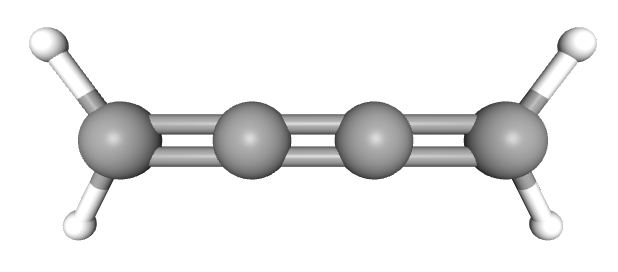
\includegraphics[width=\linewidth]{img/butatriene.png}
    \caption{Molecular structure of butatriene. Grey atoms are carbon, white are hydrogen.}
    \label{fig:butatriene}
\end{wrapfigure}

The butatriene cation is a molecule with chemical formula \(\symup{C}_4\symup{H}_4^+\) (Fig. \ref{fig:butatriene}). We wish to investigate the \textit{photoionisation} of butatriene, which can be done by plotting its ionisation or absorption spectra. This can be thought of as the energy required to ``excite'' the ground state \(S_0\) to one of two excited states \(S_1\) and \(S_2\) (Fig. \ref{fig:butatriene_excitation}).

For our propagation method, we will use MCTDH. To start a \textit{Quantics} simulation we first need to specify the Hamiltonian of the system. Here, a vibronic coupling Hamiltonian is used, in the form
\begin{equation*}
    \hat{H} = \sum_{i=1}^{18} \frac{\symit{ω}_i}{2}\paren{\frac{\partial^2}{\partial Q_i^2} + Q_i^2}\symbb{1} + \sum_{i\in G_1}\begin{bmatrix}\symit{κ}_i^{(1)} & 0 \\ 0 & \symit{κ}_i^{(2)}\end{bmatrix}Q_i + \sum_{i\in G_3}\begin{bmatrix}0 & \symit{λ}_i \\ \symit{λ}_i & 0\end{bmatrix}Q_i + \text{higher order terms} \label{eq:vibcoph} \tag{$*$}
\end{equation*}

\begin{wrapfigure}{l}{0.4\textwidth}
    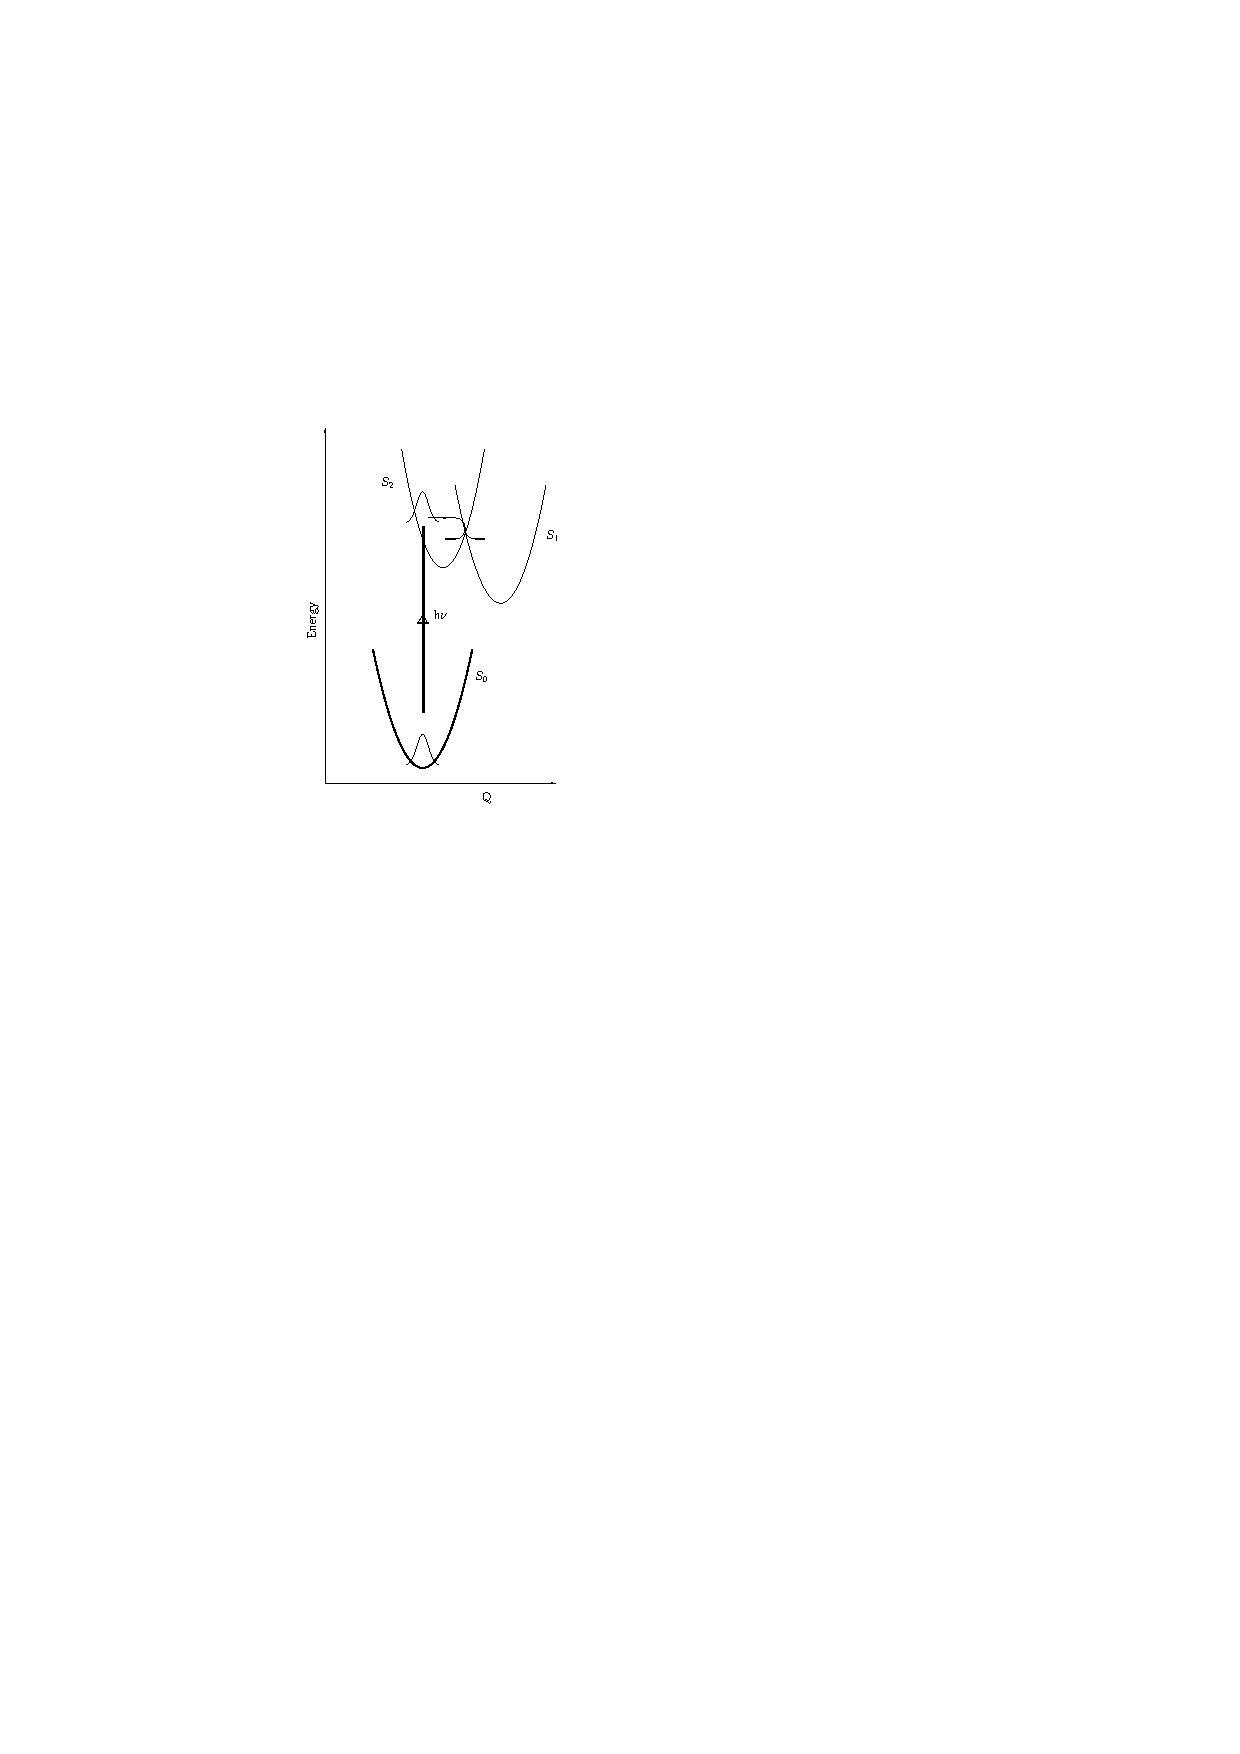
\includegraphics[page=1,width=0.4\textwidth]{img/butatriene_excitation.pdf}
    \caption{Schematic diagram of excitation in butatriene.}
    \label{fig:butatriene_excitation}
\end{wrapfigure}

The Hamiltonian is defined in an operator file, where the form of the Hamiltonian is given as well as the values of its various parameters. One of the parameters is \texttt{init\_state}, which can place the wavepacket on the upper or lower excited state. We need to run calculations for both states to obtain the full spectrum.  Then, we need to specify details such as the propagation time, the initial wavefunction as well as technical details for MCTDH such as the number of points on the grid for each degree of freedom, which is included in an input file. The contents of the operator and input files are in a particular format that \textit{Quantics} can read. For the interested reader, see appendix \S\ref{ssec:inputop} for the full listing.

If we have named our input file \texttt{butatriene.inp}, we simply need to type on the command line \texttt{quantics -mnd butatriene.inp} to perfrom the simulation. The \texttt{-mnd} flag sets the directory name with the output of the simulation the same as the name of the input. If we navigate to the newly created directory, we will see the output files from the simulation:
\newline\verb|auto      check     dvr       gridpop   input|
\newline\verb|log       op.log    oper      output    psi|
\newline\verb|restart   scratch   speed     timing    update|

Note that different files may be generated depending on parameters chosen for the propagation. We can then perform the analysis on the command line. To compute the absorption spectra we use the \texttt{autospec} command. If we do not know the parameters of the command, we can first invoke the command with the help flag, using \texttt{autospec -h}. We get the following output:

\begin{code}\begin{minted}{text}
Purpose: Computation of the spectrum by fourier-transforming
         the autocorrelation function.
         Three spectra are generated acording to the weight functions
         cos^n(pi*t/(2*T)) (n=0,1,2). The option -lin allows to use
         a second set of filters. In plspec the filters of this
         second set are enabled through the option -g3, -g4, or -g5.
         Additionally there is the weight function exp(-(t/tau)^iexp).
         The conversion factor from damping time to FWHM energy width
         is 1.32 eV fs and 2.2 eV fs for iexp=1 or 2, respectively.
         Input a zero for tau if not damping is required.

Usage : autospec [-f -i -o -e -n -r -ctr -ph -p -q -g -t -FT -EP -Mb -ver -h -? -inter] 
                [emin emax unit tau iexp]

Options : 
-f FILE : The autocorrelation is read from file FILE rather than from ./auto
           The string FILE may be a relative or full path-name.
-i DIR  : Take DIR as input directory.
...
\end{minted}
\caption{Snippet of the help text for the \texttt{autospec} program. The output is continued by further explanation of all of the parameters.}
\label{lst:autospec_help}
\end{code}

Every analysis program has an \texttt{-h} flag for this purpose. In this scenario, we would like to see the spectra between 9.0 and 10.5 eV, with a damping time of 30 fs at the first order. We can specify this only using the positional parameters \texttt{autospec 9.0 10.5 ev 30 1}. This creates another file named \texttt{spectrum.pl}, which can be read using \textit{gnuplot} using the \texttt{gnuplot} command. 

\textit{gnuplot} is also a program the functions on the command line. We pass it the \textit{gnuplot}-specific command \texttt{plot 'spectrum.pl' u 1:2 w l}, which is to create a line plot of the first column, energy, against the second, intensity. There are further columns for the intensity for a different variant of the formula, but we will use the one with the \(g_0\) damping function. This will show a popup with the resulting plot (Fig. \ref{fig:but_spectra_gnuplot}). We then repeat the simulation changing the parameter \texttt{init\_state = 2} to \texttt{1} in the input file to simulate the excitation onto the other state.

Having obtained two \texttt{spectrum.pl} files we need to add their contents together. Firstly, they must be in the same folder, which requires copying either using the \texttt{cp} command or in a file explorer. Then, we paste the contents of both files together using the command \texttt{paste spectrum1.pl spectrum2.pl > spectrumc.pl}. To view this using \textit{gnuplot}, the command \texttt{plot 'spectrumc.pl' u 1:(\$2+\$6) w l} must be used to add the second and sixth column together before plotting\footnote{A program named \texttt{sumspec} exists in the \textit{Quantics} package which can also be used to sum columns together. However, this program also has many parameters that the user needs to be familiar with.}.

Figure \ref{fig:but_spectra} shows the simulated spectra that was performed with \textit{Quantics} against the spectrum that was obtained via experiment. We see that the MCTDH calculation aligns very closely with experimental laboratory data! Note that the files given in \S\ref{ssec:inputop} and shown in Fig. \ref{fig:but_spectra_gnuplot} are for the linear terms only (equation (\ref{eq:vibcoph})), while Fig. \ref{fig:but_spectra} uses the spectrum calculated up to quadratic terms. They are similar, but the higher-order model is slightly more accurate.

\begin{figure}[h]
    \centering
    \begin{minipage}[]{.37\textwidth}
        \centering
        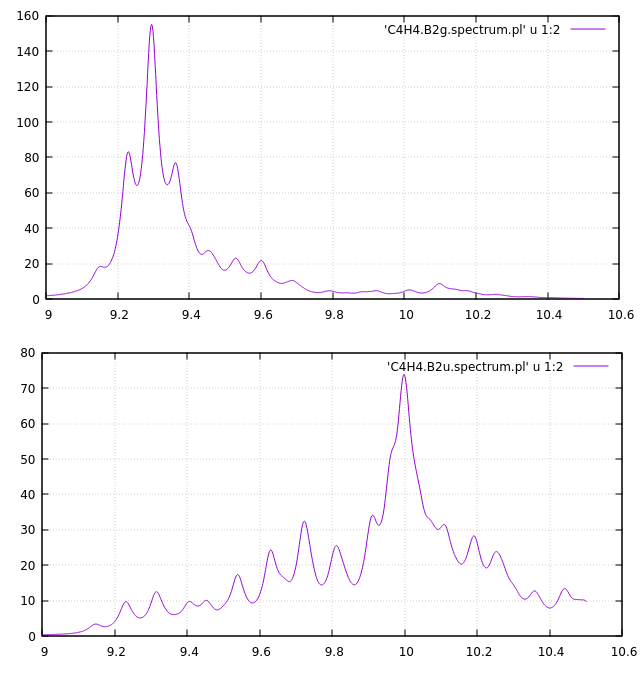
\includegraphics[width=\textwidth]{img/but_spectra.png}
        \caption{Partial spectra of excitation to each of the two excited states shown in \textit{gnuplot}. They must be added to obtain the combined spectrum in Fig. \ref{fig:but_spectra}.}
        \label{fig:but_spectra_gnuplot}
    \end{minipage}\hfill\begin{minipage}[]{.57\textwidth}
        \centering
        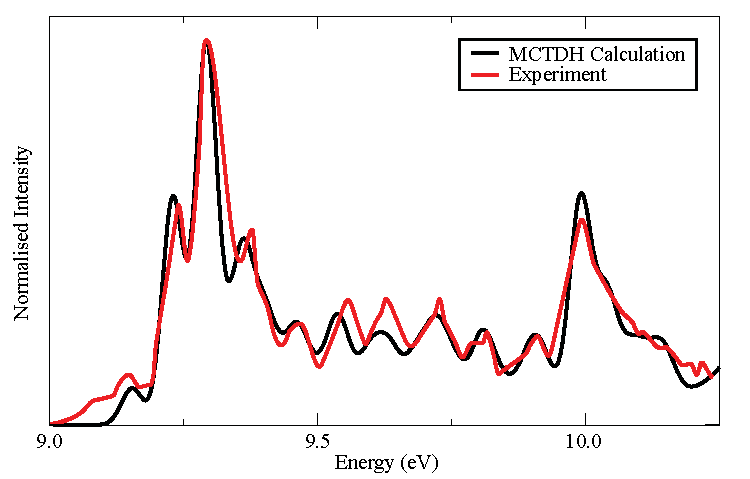
\includegraphics[page=1,width=\textwidth]{img/but_spectra.pdf}
        \caption{Calculated absorption spectrum of butatriene (quadratic model) in black,\textsuperscript{\cite{butatrienesim}} and the spectrum from an experiment.\textsuperscript{\cite{butatrieneexp}}.}
        \label{fig:but_spectra}
    \end{minipage}
\end{figure}

For this particular molecule, the two peaks at around 9.3 eV and 10 eV have a simple interpretation; they are from the populations of the lower ionic state and the higher ionic state, respectively.\textsuperscript{\cite{studying}} The intensities in the middle however, are due to \textit{vibronic states} that act as a mixture of the two states. These are formed as a result of a \textit{conical intersection} between the potential energy surfaces of the two excited states\textsuperscript{\cite{mysteryband}} (see \S\ref{sec:background}, Fig. \ref{fig:conical_intersection}).

\subsection{Aims and objectives}\label{ssec:aims}

As seen in the previous section, the use of typing in commands in the command line window is very inconvenient. If we focus on the tasks required to plot the absorption spectra, we see that the user needed to know:
\begin{itemize}
    \item The name of the required \textit{Quantics} analysis program, namely \texttt{autospec};
    \item The inputs of the analysis program, which can be seen by using the help flag \texttt{-h};
    \item The form of the output of the analysis program, namely that for the \texttt{spectrum.pl} file the first column in energy and the second is intensity (for the damping function \(g_0\));
    \item The gnuplot commands that are required to plot the values in the columns of the output.
\end{itemize}

\noindent It is clear that to performing this one analysis as a person unfamiliar with any of these tasks would be very challenging. In the past, there has been some steps in making the analysis more user-friendly.
\begin{itemize}
    \item There are a number of shell scripts, or `pl'-scripts that automatically plot the output of the analysis program in \textit{gnuplot}. The script still requires the input parameters so it can call the corresponding analysis program. There exists one called \texttt{plspec} for plotting the absorption spectra which we did not use.
    \item Some analysis programs, including \texttt{autospec}, come with an \texttt{-inter} flag (for ``interactive''), which replaces some of these parameters with a command line menu (Listing \ref{lst:showsys_menu}). These menus come as default for some other programs, e.g.~\texttt{showsys} which plots the potential energy surface (PES) or the time-evolution of the wavepacket, which may also have optional parameters, but in general must be interacted with using the command line input.
\end{itemize}

\begin{code}\begin{minted}{text}
0 = stop,  q = stop,  quit = stop
1 = plot to screen
5 = save data to an xyz file
9 = toggle re-plot (get new set of contours)

10 = change plot task (plot diabatic reduced density)
20 = change coordinate section (  Q_5=x  Q_14=y)
30 = change coordinate bounds
40 = show coordinate info
50 = change a single coordinate
60 = change state selection (  1)
80 = change coordinate units
90 = change Z-axis units (au)

110 = toggle contour mode (linear)
120 = change number of contours (21)
150 = toggle grid lines (off)
160 = toggle surface (off)
170 = toggle contour lines (on)
240 = toggle key (off)
245 = toggle title (on)
280 = change time-slice format, e.g. movie(step-through)
285 = change time-step (  1)
\end{minted}
\caption{The main command line menu of the \texttt{showsys} program. Only a subset of all the options are included.}
\label{lst:showsys_menu}
\end{code}

\begin{itemize}
    \item Finally, there is a program called \texttt{analysis}, which is a command line menu program which lists the analysis programs, and calls them (usually with \texttt{-inter}) when the user selects the option. Listing \ref{lst:analysis_menu} shows the format of this program.
\end{itemize}

\begin{code}\begin{minted}{text}
************************************************************************
     THE QUANTICS WAVEPACKET PROPAGATION ANALYSIS PACKAGE
          Program Version :     2
          Release         :     1
************************************************************************
Present directory is: {working directory}

  0 = stop
  1 = list / change directory
  2 = analyse convergence
  3 = analyse integrator
  4 = analyse results
  5 = analyse system evolution
  6 = analyse potential surface
>> 4
 *** Plot Results ***
 0 = return to main menu
 1 = Plot autocorrelation function
 2 = Plot Fourier Transform of autocorrelation function
 3 = Plot spectrum from autocorrelation function
 4 = Plot eigenvalues from matrix diagonalisation
\end{minted}
\caption{The format of the \texttt{analysis} program. Typing 2 (or 3) from here will call \texttt{autospec -inter}.}
\label{lst:analysis_menu}
\end{code}

However, we can go one step further. All the previous steps mentioned still required the use of the command line interface (CLI). However, for many people in the current day, graphical user interfaces (GUIs) are used where visual icons and buttons with labels appear on a screen that can be interacted with.\textsuperscript{\cite{risegui}} Consider the \texttt{analysis} program (Listing \ref{lst:analysis_menu})---it would be much more efficient if we can click these options instead of typing their corresponding number.

The aim of the project is the creation of such a GUI to replace the older CLI that is necessary to perform analysis in \textit{Quantics}. The GUI can present the user with the different analyses and allow them to choose the parameters of the analysis by interacting with the visuals on the screen. It should be user friendly by having a layout that is not confusing or necessitate looking up information on how to use it.

Ideally, all present analysis programs should be included as an option in the GUI. However, due to time limitations, only a subset of all programs were included, but this did include all the programs listed by the command-line \texttt{analysis} program (except the ones that did not work). Even if not all programs are included, the framework in the program should make integrating analyses as easy as possible.

A secondary aim is to create new analysis programs for \textit{Quantics}, especially for DD-vMCG simulations, which is a comparatively newer method compared to MCTDH.Implementations can be found in \S\ref{ssec:new_analysis}. An extended objective, which is to check on the status of a \textit{Quantics} simulation running on a remote server, was proposed, but never completed due to time limitations.

\subsection{Software development basis}\label{ssec:dev}

It is not a good idea to implement a GUI from scatch, as there are a number of packages and frameworks that already exist to help in the GUI implementation. The framework chosen is \textit{PyQt}\footnote{\url{https://riverbankcomputing.com/software/pyqt}}, which provides Python bindings to the underlying C++ code of Qt, a powerful cross-platform GUI framework.

One might consider why not to use the C++ interface directly, since this would be faster. The reason is because we can use \textit{pyqtgraph} (further disscused in \S\ref{ssec:plot_widget}) to natively insert a plotting tool inside the GUI, without needing to call other programs such as \textit{gnuplot}. \textit{pyqtgraph} is not available in C++, so Python is therefore the programming language used for this project.

\textit{PyQt} has advantages over other GUI frameworks due to its size and power; for example, it includes 200 widgets, which are representations of an item on a screen.\textsuperscript{\cite{pyqt}} There is also a dedicated program called \textit{Qt Designer}, which helps programmers to design a UI visually as seen by the user (\S\ref{ssec:ui_design}). \textit{Qt} itself has been used for software such as VLC media player\footnote{\url{https://code.videolan.org/videolan/vlc}}, OBS, for screencasting and recordings\footnote{\url{https://github.com/obsproject/obs-studio}}, and is also the underlying basis of \textit{Spyder}\footnote{\url{https://github.com/spyder-ide/spyder}}, the integrated development environment (IDE) tailored for scientific computing that I use to write Python code.

The code development of the project uses \textit{Git}, a revision control software which allows previous versions of the program to be easily accessed, and newly introduced code can be reverted if it breaks the program.\textsuperscript{\cite{git}} Each new change can be added to a ``commit'' which is recorded as a snapshot of the program, and the history of commits (the log) can be used to see the history of what has been implemented.

\begin{figure}[h]
    \centering
    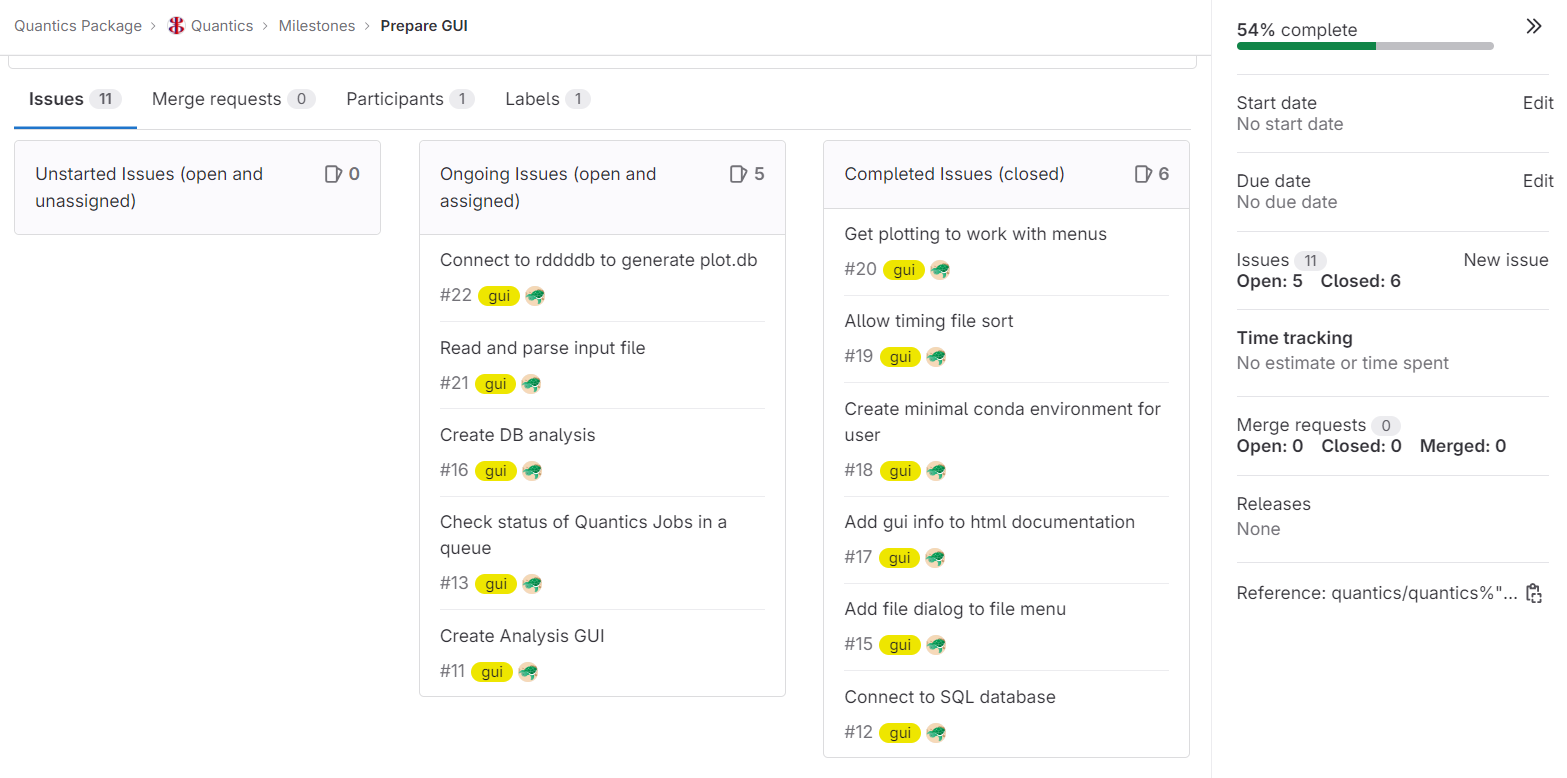
\includegraphics[width=0.9\textwidth]{img/gitlab.png}
    \caption{The \textit{GitLab milestone}, which consists of tasks set out to complete, for this project.}
    \label{fig:gitlab}
\end{figure}

\textit{Git} is also related to \textit{GitLab}, a hosting service for software projects, which allows collaborative work between different authors, with features such as \textit{milestones} to distribute tasks to different people (for this project, all were to me). A centralised repository of code can be hosted on \textit{GitLab}, which can then be downloaded locally on a computer. Using \textit{Git}, code can then by comitted and ``pushed'' back onto the online repository, and changes can be seen by other people. Code can also be committed onto different ``branches'', which allows parallel, non-linear development of the code, which can be merged together if necessary. A branch named \texttt{analysis\_gui} is dedicated to the code created in this project.

\subsection{Dissertation layout}\label{ssec:diss_layout}

In \S\ref{sec:background}, methods for solving the time-dependent Schr\"odinger equation in \textit{Quantics} are discussed. The design of the GUI and base structure of the code are explained in \S\ref{sec:design}. \S\ref{sec:implementation} is dedicated to the implementation of individual features and analysis of the GUI. The documentation and testing of the code are described in \S\ref{sec:doc_test}. The conclusion \S\ref{sec:conclusion} will then detail a summary of how the aims of the project are met, any limitations to the work and how the code can be improved upon in the future.

\section{Background}\label{sec:background}

\subsection{The Schr\"odinger equation}\label{ssec:schrodinger}

For a quantum dynamics simulation to function, it must know the equations of motion for the system. These are obtained by solving the Schr\"odinger equation, which is akin to Newton's second law in classical mechanics. There are two forms of this equation. In its time-dependent form, it is the time-dependent Schr\"odinger equation (TDSE) and reads
\begin{equation}
    i\hbar\frac{\partial\symit{Ψ}}{\partial t} = \hat{H}\symit{Ψ} \label{eq:tdse}
\end{equation}
while in its time-independent form (TISE), reads
\begin{equation}
    \hat{H}\symit{Ψ}_n = E_n\symit{Ψ}_n. \label{eq:tise}
\end{equation}
The term \(\hat{H}\) is known as the Hamiltonian operator. It represents the total energy of the system, but also governs the time evolution of quantum states.\textsuperscript{\cite{introquantum}} If the Hamiltonian is time-dependent, for example, due to an external laser field, the time-dependent version must be used. Otherwise, both equations are equivalent, and in the case of quantum dynamics simulations, which approach to take depends on numerical efficiency.

Equation (\ref{eq:tdse}) represents an initial value problem (IVP), while equation (\ref{eq:tise}) represents an eigenvalue problem. Mathematically, IVPs are simpler but the TDSE has one additional variable, time. Historically, the TISE was preferred, but the TDSE is now generally preferred; some reasons include better approximations, being simpler than the TISE for certain processes containing continuum functions, and only requiring the properties of the initial state, whose restriction makes the problem easier to solve.\textsuperscript{\cite{studying}}

In the time-dependent scheme, the wavefunction \(\symit{Ψ}\) can be decomposed into wavepackets. The solution of the TDSE generates methods to propagate these wavepackets.\textsuperscript{\cite{wavepacket}} However, the TDSE (\ref{eq:tdse}) cannot be analytically solved for more than two particles, similarly to the three-body problem in classical mechanics. Thus, numerical methods and approximations are used to produce solutions, and the accuracy of such methods can then be experimentally verified in a laboratory.

One such approximation is known as the Born-Oppenheimer approximation, which operates in what is known as the \textit{adiabatic} picture. It operates from an assumption that the nuclear and electronic motions of the atom can be seperated. This leads to the idea of a molecular system moving over a potential energy surface (PES), to which the analysis allows many quantum features to be described---for example, the minima represent stable configurations and saddle points represent transition states connecting these configurations.\textsuperscript{\cite{multiquantdyn}}

A method that solves the TDSE, known as the multiconfiguration time-dependent Hartree (MCTDH) method, is the core method of the \textit{Quantics} package. It is designed to tackle multidimensional problems with many degrees of freedom and still produce accurate results in line with experimental data (e.g. Figure \ref{fig:but_spectra}). The following sections detail the mathematical description of MCTDH, as well as some of its applications. \S\ref{ssec:standardmethod} and \S\ref{ssec:tdh} are predecessors to MCTDH as well as limits to MCTDH given certain circumstances. The mathematics of MCTDH are then given in \S\ref{ssec:mctdh}. An overview of ML-MCTDH, an extension to MCTDH, is given in \S\ref{ssec:mlmctdh}. Finally, the \textit{Quantics} package also implements the direct dynamics variational multi-configurational Gaussian method (DD-vMCG), which calculates potential surfaces on the fly. This is briefly discussed in \S\ref{ssec:ddvmcg}.

\subsection{The standard method}\label{ssec:standardmethod}

In these following sections, atomic units are used where \(\hbar = 1\). The time-dependent Schr\"odinger equation previously introduced in (\ref{eq:tdse}) thus reads
\begin{equation}
    i\frac{\partial\symit{Ψ}}{\partial t} = i\dot{\symit{Ψ}} = \hat{H}\symit{Ψ}. \label{eq:tdse2}
\end{equation}

A direct way to solve equation (\ref{eq:tdse2}), known as the ``standard method'', is to expand the \(f\)-dimensional wavefunction \(\symit{Ψ}\) into a product of time-independent basis sets per
\begin{equation}
    \symit{Ψ}(q_1, \dots, q_f; t) = \sum_{j_1=1}^{N_1} \cdots \sum_{j_f=1}^{N_f} C_{j_1,\dots, j_f}(t) \prod_{k=1}^f \symit{χ}_{j_k}^{(k)}(q_k) \label{eq:standardmethod}
\end{equation}
where \(f\) is the number of degrees of freedom, \(q_1, \dots, q_f\) are the nuclear coordinates, \(C_{j_1,\dots, j_f}(t)\) are the expansion coefficients, \(\symit{χ}_{j_k}^{(k)}\) are the basis functions for DOF \(k\) and \(N_k\) is the number of basis functions employed for DOF \(k\).\textsuperscript{\cite{mctdh}}

The equations of motion for the system can be derived using the Dirac-Frenkel variational principle,\textsuperscript{\cite{diracfrenkel}} which reads
\begin{equation}
    \bra{δ\symit{Ψ}}\hat{H}\ket{\symit{Ψ}} - i\angled{δ\symit{Ψ}|\dot{\symit{Ψ}}} = 0 \label{eq:diracfrenkel}
\end{equation}
where we have
\begin{align}
    δ\symit{Ψ} &= \sum_{l_1,\dots, l_f}\frac{\partial\symit{Ψ}}{\partial C_{l_1,\dots, l_f}}δC_{l_1,\dots, l_f} = \sum_{l_1,\dots, l_f}\prod_{k=1}^f \brackets{\symit{χ}_{l_k}^{(k)}(q_k)}δC_{l_1\cdots l_f}, \\
    \dot{\symit{Ψ}} &= \sum_{j_1,\dots, j_f} \dot{C}_{j_1,\dots, j_f}(t) \prod_{k=1}^f \symit{χ}_{j_k}^{(k)}(q_k).
\end{align}
Since variations are independent,
\begin{equation*}
    δC_{l_1,\dots, l_f} = \begin{cases}1 & \text{for } l_1,\dots, l_f = l_1^{(0)},\dots l_f^{(0)} \\ 0 &\text{otherwise}\end{cases}
\end{equation*}
which after replacing \(l_k^{(0)}\) with \(l_k\) and applying (\ref{eq:diracfrenkel}), then results in the equations of motion for \(C_{j_1,\dots, j_f}(t)\):
\begin{equation}
    i\dot{C}_{j_1,\dots,j_f} = \sum_{l_1,\cdots,l_f} \big\langle\symit{χ}_{j_1}^{(1)}\cdots\symit{χ}_{j_f}^{(f)}\big\vert\, H\,\big\vert\symit{χ}_{l_1}^{(1)}\cdots\symit{χ}_{l_f}^{(f)}\big\rangle C_{l_1,\cdots,l_f}
\end{equation}
which is a first-order differential equation with constant coefficients in the form\textsuperscript{\citep[chap.~8.1]{quandymchem}}
\begin{equation}
    \symbfit{C}(t) = e^{-i\symbf{H}t}\symbfit{C}(0).
\end{equation}

This method is numerically exact. However, it also scales exponentially with the number of degrees of freedom: for \(N\) basis points and \(f\) degrees of freedom, the computational cost is of the order \(N^f\), which provides an effective limit of four-atom systems using this method.\textsuperscript{\cite{quanticsreview}}

\subsection{The time-dependent Hartree method}\label{ssec:tdh}

One of the alternatives to the standard method in \S\ref{ssec:standardmethod} is the time-dependent Hartree method,\textsuperscript{\cite{tdh, tdh2}} where the wavefunction is expressed as a product of 1D single-particle functions (SPFs) \(\symit{φ}_k\),
\begin{equation}
    \symit{Ψ}(q_1,\dots q_f; t) = a(t)\prod_{k=1}^f \symit{φ}_k(q_k, t).\label{eq:hartreeprod}
\end{equation}
The product of functions, known as a \textit{Hartree product}, is now time-dependent as opposed to the time-independence in the standard method. \(a(t)\) is a redundant term which allows us to freely choose the phases of the SPFs, and SPFs usually take the form in a time-independent basis set of primitive basis functions \(\symit{χ}_{i_k}^{(k)}(q_k)\)
\begin{equation}
    \symit{φ}_{j_k}^{(k)}(q_k, t) = \sum_{i_k = 1}^{N_k} c_{i_k}^{(k, j_k)}(t)\symit{χ}_{i_k}^{(k)}(q_k). \label{eq:spfs}
\end{equation}
The representation of \(\symit{Ψ}\) in equation (\ref{eq:hartreeprod}) is not unique---take for example, \(\symit{φ}_1\cdot\symit{φ}_2 = (\symit{φ}_1/b)(\symit{φ}_2\cdot b)\) for any complex number \(b\neq 0\). Thus we introduce constraints
\begin{equation}
    i\angled{\symit{φ}_k(t) | \dot{\symit{φ}}_k(t)} = g_k(t)
\end{equation}
for an arbitary real function \(g_k(t)\). The constraint also ensures the norm of the SPFs are conserved since
\begin{equation}
    \frac{\symup{d}}{\symup{d}t}||\symit{φ}_k||^2 = \angled{\dot{\symit{φ}}_k | \symit{φ}_k} + \angled{\symit{φ}_k | \dot{\symit{φ}}_k} = 2\operatorname{Im}g_k = 0.
\end{equation}

To prepare for the variation, and for convenience, definining
\begin{equation*}
    \symit{Φ} := \prod_{k=1}^f \symit{φ}_k, \qquad \symit{Φ}^{(k)} := \prod_{l=1, l\neq k}^f \symit{φ}_l
\end{equation*}
we have
\begin{align}
    \dot{\symit{Ψ}} &= \dot{a}(t)\symit{Φ} + a\sum_{k=1}^f \dot{\symit{φ}}_k\symit{Φ}^{(k)}, \\
    δ\symit{Ψ} &= (δa)\symit{Φ} + a\sum_{k=1}^f (δ\symit{φ}_k)\symit{Φ}^{(k)}.
\end{align}
Applying (\ref{eq:diracfrenkel}) to the above, we obtain terms with \(δ a\) and terms with \(δ \symit{φ}_k\), which must equal 0 independently since they are independent of each other:
\begin{align}
    \bra{(δa)\symit{Φ}}\hat{H}\ket{a\symit{Φ}} - i\langle(δa)\symit{Φ}\mid\dot{a}\symit{Φ} + a\sum_{k}\dot{\symit{φ}}_k\symit{Φ}^{(k)}\rangle &= 0, \label{eq:tdhda}\\
    \sum_{k=1}^f \Bigl[\big\langle(δ\symit{φ}_k)a\symit{Φ}^{(k)}\big\vert\, \hat{H}\,\big\vert a\symit{Φ}\big\rangle - i\big\langle(δ\symit{φ}_k)a\symit{Φ}\,\big\vert\,\dot{a}\symit{Φ} + a\sum_{k'}\dot{\symit{φ}}_k \symit{Φ}^{(k')}\big\rangle\Bigr] &= 0. \label{eq:tdhdphi}
\end{align}
For (\ref{eq:tdhda}), this simplifies to
\begin{align}
    (δa)^* a\bra{\symit{Φ}}H\ket{\symit{Φ}} &= i(δa)^*\dot{a} + i(δa)^* a\sum_{k}\angled{\symit{Φ}\big\vert\dot{\symit{φ}}_k\symit{Φ}^{(k)}} \nonumber \\
    i\dot{a} &= (E - \sum_{k=1}^f g_k)a
\end{align}
since \(\angled{\symit{Φ}\,\big\vert\,\dot{\symit{φ}}_k\symit{Φ}^{(k)}} = i\angled{\symit{φ}|\dot{\symit{φ}}} = g_k\) and introducing
\begin{equation}
    E = \bra{\symit{Φ}}\hat{H}\ket{\symit{Φ}} = \frac{\bra{\symit{Ψ}}\hat{H}\ket{\symit{Ψ}}}{\angled{\symit{Ψ}|\symit{Ψ}}}.
\end{equation}
For (\ref{eq:tdhdphi}), we have the simplifications
\begin{align}
    \bra{(δ\symit{φ}_k)a\symit{Φ}^{(k)}}\hat{H}\ket{ a\symit{Φ}} &= i\langle(δ\symit{φ}_k)a\symit{Φ}\mid\dot{a}\symit{Φ}\rangle + i\langle(δ\symit{φ}_k)a\symit{Φ}\mid a\sum_{k'}\dot{\symit{φ}}_k \symit{Φ}^{(k')}\rangle \nonumber\\
    |a|^2\bra{δ\symit{φ}_k}\bra{\symit{Φ}^{(k)}}\hat{H}\ket{\symit{Φ}^{(k)}}\ket{\symit{φ}_k} &= i\dot{a}a^*\angled{δ\symit{φ}_k|\symit{φ}_k} + i|a|^2\angled{δ\symit{φ}_k|\dot{\symit{φ}}_k} + i|a|^2\angled{δ\symit{φ}_k|\symit{φ}_k}\sum_{k'\neq k}\angled{\symit{φ}_{k'}|\dot{\symit{φ}}_{k'}} \nonumber\\
    |a|^2\bra{δ\symit{φ}_k}\hat{\symscr{H}}^{(k)}\ket{\symit{φ}_k} &= |a|^2(E-\sum_k g_k)\angled{δ\symit{φ}_k|\symit{φ}_k} + i|a|^2\angled{δ\symit{φ}_k|\dot{\symit{φ}}_k} + |a|^2\angled{δ\symit{φ}_k|\symit{φ}_k}\sum_{k'\neq k}g_{k'} \nonumber \\
    i\angled{δ\symit{φ}_k|\dot{\symit{φ}}_k} &= \bra{δ\symit{φ}_k}\hat{\symscr{H}}^{(k)}\ket{\symit{φ}_k} - (E - g_k)\angled{δ\symit{φ}_k|\symit{φ}_k}
\end{align}
where the \textit{mean field} operator \(\hat{\symscr{H}}^{(k)} = \angled{\symit{Φ}^{(k)}|\hat{H}|\symit{Φ}^{(k)}}\) is introduced. Since \(δ\symit{φ}_k\) is arbitrary,
\begin{equation}
    i\dot{\symit{φ}_k} = (\symscr{H}^{(k)} - E + g_k)\symit{φ}_k.
\end{equation}

The choice of the function \(g_k\) can be chosen to be any real function; for Hermitian Hamiltonians one may choose \(g_k = E\) or \(g_k = E/f\) but the simplest choice is \(g_k = 0\) in which the equations of motion become
\begin{equation}
    \left\{\begin{aligned}
        a(t) &= a(0)e^{-i\int_0^t E(t')\,\symup{d}t'} \\
        i\dot{\symit{φ}}_k &= (1 - \ket{\symit{φ}_k}\bra{\symit{φ}_k})\hat{\symscr{H}}^{(k)}\symit{φ}_k
    \end{aligned}\right.
\end{equation}
where \(\ket{\symit{φ}_k}\bra{\symit{φ}_k}\) denote the projector onto state \(\symit{φ}_k\). The form of the wavefunction in (\ref{eq:hartreeprod}) simplifies one \(f\)-dimensional differential equation into \(f\) 1-dimensional differential equations, meaning the computational cost is reduced from \(N^f\) in the standard method to a mere \(N\cdot f\). As such, this method is approximate, only being exact if the Hamiltonian is seperable, i.e.~\(V_\text{corr} = 0\) in
\begin{equation}
    \hat{H} = \sum_{k=1}^f h^{(k)} + V_\text{corr}
\end{equation}
where \(h^{(k)}\) only operates on DOF \(k\). To investigate the error, consider the TDH as the solution to the TDSE with an effective Hamiltonian
\begin{equation}
    i\dot{\symit{Ψ}} = \hat{H}_\text{eff}\symit{Ψ}.
\end{equation}
It can be shown that 
\begin{align}
    \hat{H} - \hat{H}_\text{eff} = V_\text{corr} - E_\text{corr} - \sum_{k=1}^f\Bigl(\langle\prod_{k'\neq k} \symit{φ}_{k'}|\,V_\text{corr}\,|\prod_{k'\neq k} \symit{φ}_{k'}\rangle - E_\text{corr}\Bigr)
\end{align}
where \(E_\text{corr} = {}^{\bra{\symit{Ψ}}V_\text{corr}\ket{\symit{Ψ}}}/_{\angled{\symit{Ψ}|\symit{Ψ}}}\).\textsuperscript{\citep[chap.~8.2]{quandymchem}} The method has been used in the simulations of many-atom systems consisting of \(\approx 100\) modes, involving phenomena such as photodissociation and electron photodetachment.\textsuperscript{\cite{tdhapp}} However, due to the lack of correlation between the DOFs, the TDH approach is not suitable for the majority of applications, such as the \(\symup{H} + \symup{H}_2\) molecular system,\textsuperscript{\cite{tdhapp2}} as several configurations are required. This naturally leads to the multiconfiguration time-dependent Hartree method (MCTDH) in \S\ref{ssec:mctdh}.

\subsection{The multiconfiguration time-dependent Hartree method}\label{ssec:mctdh}

In order to recover some the missing correlation in TDH, we turn to using multiple configurations. First, we have the multiconfigurational wave function in the form\textsuperscript{\cite{mctdh1990}}
\begin{equation}
    \symit{Ψ}(q_1,\dots q_f; t) = \sum_{j_1=1}^{n_1} \cdots \sum_{j_f = 1}^{n_f} A_{j_1,\dots, j_f}(t)\prod_{k=1}^f \symit{φ}_{j_k}^{(k)}(q_k, t) \label{eq:mctdhwf}
\end{equation}
where the SPFs are in the same form as in TDH (\ref{eq:spfs}). Both TDH and the standard method are limits to this wavefunction. If \(n_i = 1\) for \(i = 1, \dots, f\), this is equivalent to TDH, and if \(n_i = N_i\) for \(i = 1, \dots, f\) then this is equivalent to the standard method. MCTDH can therefore be considered to fully cover the range of approximations from TDH to an numerically exact solution as \(n_i\) is increased from 1 to \(N_i\).\textsuperscript{\cite{mctdh}} Like in the TDH approach, (\ref{eq:mctdhwf}) is not a unique representation as one can perform a linear transformation on the SPFs then perform its inverse transformation onto \(A\). The constraints here are
\begin{equation}
    i\angled{\symit{φ}_j^{(k)}(t)\big\vert\dot{\symit{φ}}_l^{(k)}(t)} = \bra{\symit{φ}_j^{(k)}(t)}g^{(k)}\ket{\symit{φ}_l^{(k)}(t)} \qquad \angled{\symit{φ}_j^{(k)}(0)\big\vert\symit{φ}_l^{(k)}(0)} = \symit{δ}_{jl}.
\end{equation}
It is assumed that \(g^{(k)} = 0\) in this section for simplicity, but it is possible to derive the MCTDH equations of motion for a general \(g^{(k)} \neq 0\) with more algebra.\textsuperscript{\citep[chap.~8.8]{quandymchem}} For convenience, we define composite indices as
\begin{align*}
    J &:= j_1,\dots, j_f \\
    J^k &:= j_1,\dots, j_{k-1}, j_{k+1}, \dots, j_f \\
    J_l^k &:= j_1,\dots j_{k-1}, l, j_{k+1}, \dots, j_f
\end{align*}
and configurations as
\begin{equation*}
    \symit{Φ}_J := \prod_{k=1}^f \symit{φ}_{j_k}^{(k)} \qquad \symit{Φ}_{J^k} := \prod_{k'=1,k'\neq k}^f \symit{φ}_{j_{k'}}^{(k')}.
\end{equation*}
This allows us to define \textit{single-hole functions}, which represent the product of SPFs that do not contain the SPF for DOF \(k\), as
\begin{equation}
    \symit{Ψ}_l^{(k)} = \sum_{J^k}A_{J_l^k}\symit{Φ}_{J^k}
\end{equation}
thus allowing the MCTDH wavefunction (\ref{eq:mctdhwf}) to be written as
\begin{equation}
    \symit{Ψ} = \sum_J A_J\symit{Φ}_J = \sum_{l}\symit{φ}_l^{(k)}\symit{Ψ}_l^{(k)}. \label{eq:mctdhwf2}
\end{equation}
for any \(k=1,\dots, f\), as well as the mean fields
\begin{equation}
    \langle\hat{H}\rangle_{jl}^{(k)} = \bra{\symit{Ψ}_j^{(k)}}\hat{H}\ket{\symit{Ψ}_l^{(k)}}
\end{equation}
and \textit{density matrices}
\begin{equation}
    \symit{ρ}_{jl}^{(k)} = \angled{\symit{Ψ}_j^{(k)}\big\vert\symit{Ψ}_l^{(k)}} = \sum_{J^k} A_{J_j^k}^* A_{J_l^k}.
\end{equation}
to be defined. The density matrix is related to the density operator
\begin{equation}
    \rho^{(k)}(q_k, q_k') = \sum_{j,l}^{n_k}\symit{φ}_{j}^{(k)}(q_k)\symit{ρ}_{lj}^{(k)}\symit{φ}_{l}^{(k)}(q_k'),
\end{equation}
whose diagonal values highlight how the wavepacket moves along the coordinate \(k\). Furthermore, the diagonalisation of the density operator also gives the \textit{natural populations} (eigenvalues) and \textit{natural orbitals} (eigenvactors). A small natural population indicates the converge of MCTDH.\textsuperscript{\cite{densmat}}

The variation and time differentiation of (\ref{eq:mctdhwf2}) can be calculated as
\begin{equation}
    δ\symit{Ψ} = \symit{Φ}_J\, δA_J = \symit{Ψ}_j^{(k)}\, δ\symit{φ}_j^{k}
\end{equation}
and
\begin{equation}
    \dot{\symit{Ψ}} = \sum_J \dot{A}_J\symit{Φ}_J + \sum_{k=1}^f \sum_{j=1}^{n_k} \dot{\symit{φ}}_j^{(k)} \symit{Ψ}_j^{(k)}.
\end{equation}
Applying the variational principle (\ref{eq:diracfrenkel}) we first have the variation of \(A_J\),
\begin{align}
    \bra{\symit{Φ}_J}\hat{H}\ket{\symit{Ψ}} &= i\angled{\symit{Φ}_J|\dot{\symit{Ψ}}} \nonumber \\
    \sum_L \bra{\symit{Φ}_J}\hat{H}\ket{\symit{Φ}_L} A_L &= i\sum_L \angled{\symit{Φ}_J|\dot{A}_L\symit{Φ}_L} + i \sum_k \sum_l \angled{\symit{Φ}_J|\dot{\symit{φ}}_l^{(k)}\symit{Ψ}_l^{(k)}} \nonumber\\
    &= i\dot{A}_J + i\sum_k\sum_l \angled{\symit{φ}_{j_k}^{(k)}\big\vert\dot{\symit{φ}}_l^{(k)}}\angled{\symit{Φ}_{J^k}\big\vert\symit{Ψ}_l^{(k)}} = i\dot{A}_J.
\end{align}
Then comes the variation of \(\symit{φ}_j^{(k)}\),
\begin{align}
    \big\langle\symit{Ψ}_j^{(k)}\big\vert\, \hat{H}\,\big\vert\symit{Ψ}\big\rangle &= i\sum_L \angled{\symit{Ψ}_j^{(k)}|\symit{Φ}_L}\dot{A}_L + i\sum_L\big\langle\symit{Ψ}_j^{(k)}\big\vert\sum_{m}\sum_{l}\dot{\symit{φ}}_l^{(m)}\symit{Ψ}_l^{(m)}\big\rangle \nonumber\\
    \big\langle\symit{Ψ}_j^{(k)}\big\vert\, \hat{H}\,\big\vert\sum_l\symit{Ψ}_l^{(k)}\symit{φ}_l^{(k)}\big\rangle &= \sum_L \angled{\symit{Ψ}_j^{(k)}|\symit{Φ}_L}\dot{A}_L \bra{\symit{Φ}_L}\hat{H}\ket{\symit{Ψ}} + i\big\langle\symit{Ψ}_j^{(k)}\big\vert\sum_l\dot{\symit{φ}}_l^{(k)}\symit{Ψ}_l^{(k)}\big\rangle \nonumber\\
    \sum_l \langle\hat{H}\rangle_{jl}^{k}\symit{φ}_l^{(k)} &= \hat{P}^{(k)}\sum_l\langle\hat{H}\rangle_{jl}^{k}\symit{φ}_l^{(k)} + i\sum_l \symit{ρ}_{jl}^{(k)}\dot{\symit{φ}}_l^{(k)} \nonumber\\
    i\dot{\symit{φ}}_j^{(k)} &= \sum_{m,l}(\symit{ρ}_{jm}^{(k)})^{-1} (1-\hat{P}^{(k)})\langle\hat{H}\rangle_{ml}^{k}\symit{φ}_l^{(k)}
\end{align}
where we defined the MCTDH projector as
\begin{equation}
    \hat{P}^{(k)} = \sum_{j=1}^{n_k} \ket{\symit{φ}_j^{(k)}}\bra{\symit{φ}_j^{(k)}}.
\end{equation}
If we also define vectors of SPFs as
\begin{equation}
    \symbfit{φ}^{(k)} = (\symit{φ}_1^{(k)},\dots,\symit{φ}_{n_k}^{(k)})^{\symsf{T}}
\end{equation}
then the MCTDH equations of motion for \(g^{(k)} = 0\) become\textsuperscript{\citep[chap.~8.3]{quandymchem}}
\begin{equation}
    \left\{\begin{aligned}
        i\dot{A}_J &= \sum_L \bra{\symit{Φ}_J}\hat{H}\ket{\symit{Φ}_L} A_L \\
        i\dot{\symbfit{φ}}^{(k)} &= (1-\hat{P}^{(k)})(\symbfit{ρ}^{(k)})^{-1}\angled{\symbf{H}}^{(k)}\symbfit{φ}^{(k)}. \label{eq:mctdheom}
    \end{aligned}\right.
\end{equation}
These equations are in the form of a coupled non-linear differential equation, which can be solved using a numerical integration scheme such as Runge–Kutta, or a specialised scheme known as constant mean field.\textsuperscript{\cite{cmf}}
MCTDH has been used to investigate many phenomena such as photodissociation processes (e.g.~in \(\symup{NOCl}\)\textsuperscript{\cite{nocl}}, \(\symup{NO}_2\)\textsuperscript{\cite{no2}}), molecule surface scattering (e.g.~for \(\symup{H}_2/\symup{LiF}\)\textsuperscript{\cite{h2lif}}), the hydrogen exchange reaction \(\symup{H}+\symup{H}_2 \longrightarrow \symup{H}_2 + \symup{H}\),\textsuperscript{\cite{hh2}} and the photo-excitation of pyrazine, whose calculation included 24 nuclear degrees of freedom.\textsuperscript{\cite{pyrazine}}

The computational effort for MCTDH generally scales per \(fnN + n^f\), where \(N\) is the grid length and \(n\) the number of SPFs. As such, it still suffers from exponential scaling, but the base of the exponent can be reduced in certain ways. The following section, \S\ref{ssec:mlmctdh}, details mode combination and multilayer MCTDH, which aim to reduce the computational effort.

\subsection{Mode combination and multilayer MCTDH} \label{ssec:mlmctdh}

The SPFs introduced in (\ref{eq:spfs}) do not need to depend on a single DOF. By combining coordinates as
\begin{equation}
    Q_k = (q_{k,1}, q_{k,2}, \dots, q_{k,d})
\end{equation}
we introduce \textit{logical coordinates} (also known as ``particles''), where the \(k\)\textsuperscript{th} logical coordinate depends on \(d\) physical coordinates, such that the SPFs can be written as
\begin{equation}
    \symit{φ}_{j_k}^{(k)}(Q_k, t) = \sum_{i_1 = 1}\cdots\sum_{i_d = 1} C_{i_1,\dots,i_d}^{(k, j_k)}(t)\symit{χ}^{(k, 1)}(q_{k, 1})\cdots \symit{χ}^{(k, d)}(q_{k, d}).
\end{equation}
The wavefunction is still identical to (\ref{eq:mctdhwf}) except it now runs over the logical coordinates up to \(p\) instead over the total number of DOFs \(f\). This is known as \textit{mode combination}.

Using this method, MCTDH's \(A\)-vector can be made considerably smaller but the SPFs being multidimensional means they are harder to propagate. In general, only DOFs with strong coupling should be combined, as ``over-combining'' means propagation of the SPFs will take much longer than the propagation of the \(A\)-vector. The computational effort with mode combination is \(p\tilde{n}N^d + \tilde{n}^p\), where we see the number of DOFs \(f\) changed to the number of mode combinations \(p\) and since the grid is now multidimensional, \(N\to N^d\). If \(\tilde{n} = n^d\), the \(A\)-vector length stays identical and nothing is gained. As a rule of thumb, picking \(\tilde{n}\) such that \(\tilde{n} \approx d\cdot n\) gives a good balance.\textsuperscript{\cite{studying}}

However, there is a technique to propagate multidimensional wavefunctions efficiently which we already know: MCTDH. Instead of using MCTDH to only propagate the wavefunction, we propagate the SPFs using MCTDH as well. This technique is known as multilayer MCTDH, or ML-MCTDH.\textsuperscript{\cite{ml1}} Here, the wavefunction is similar to  normal MCTDH,
\begin{equation}
    \symit{Ψ}(Q_1^1,\dots, Q_p^1; t) = \sum_{j_1=1}^{n_1} \cdots \sum_{j_p = 1}^{n_p} A_{j_1,\dots, j_p}^1(t)\prod_{k=1}^p \symit{φ}_{j_k}^{(1:k)}(Q_k^1, t)
\end{equation}
where the superscript \(1\) refers to the top layer of SPFs, but the SPFs recursively depend on the next layer of SPFs,
\begin{equation}
    \symit{φ}_m^{(l:k)}(Q_k^l, t) = \sum_{i_1=1} \cdots \sum_{i_{d_k} = 1} A_{m:i_1,\dots,i_{d_k}}^{l+1:k}(t)\symit{φ}_{i_1}^{(l+1:k, 1)}(Q_1^{l+1:k}, t)\cdots\symit{φ}_{i_{d_k}}^{(l+1:k, d_k)}(Q_{d_k}^{l+1:k}, t)
\end{equation}
where \(l\) refers to the layer and at the last layer the SPFs are the basis functions instead.\textsuperscript{\cite{ml2}} There is now an equation of motion in each layer, with the form of projector, density matrix, and mean field now depending on the layer. They have a similar form to the normal MCTDH equations of motion (\ref{eq:mctdheom}), but the calculation of the density matrices and mean-fields are more involved, since they are also calculated recursively.\textsuperscript{\cite{mleom}}

\begin{figure}[h]
    \centering
    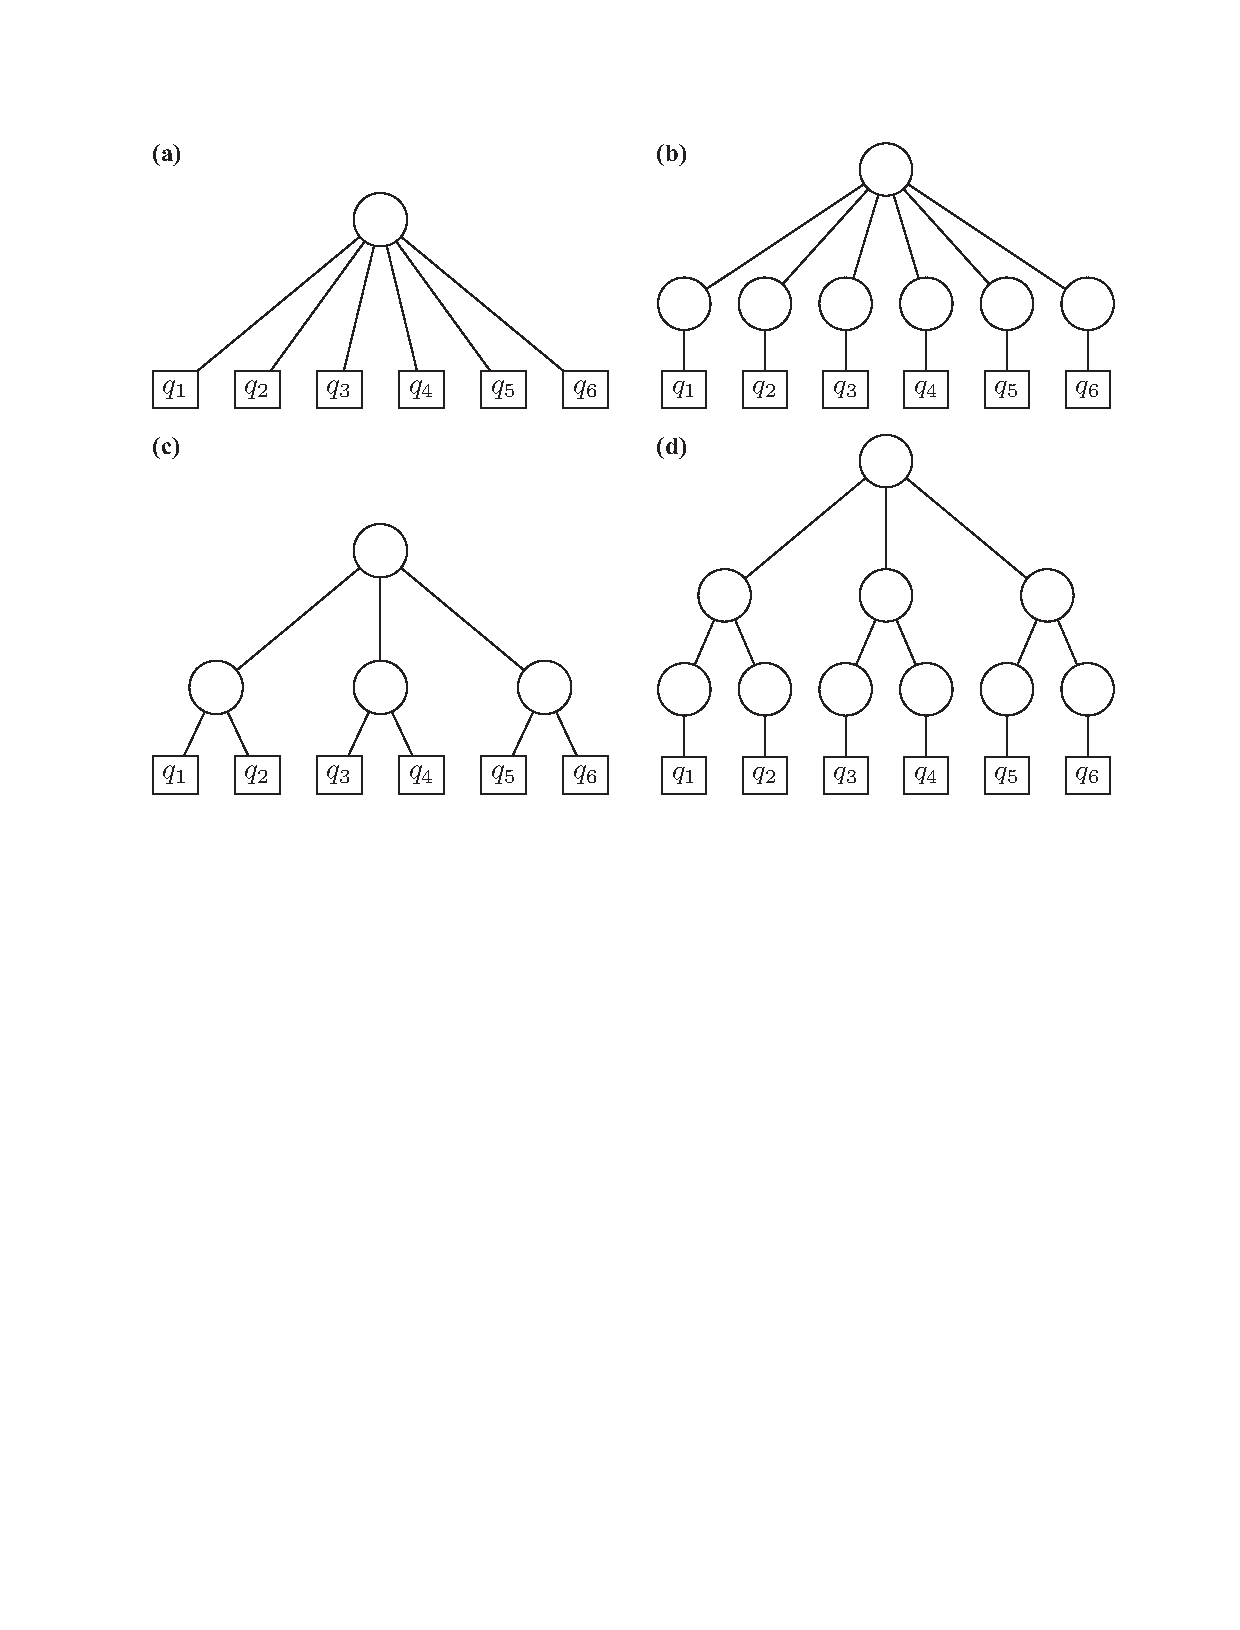
\includegraphics[page=1,width=\textwidth]{img/mcdth_trees.pdf}
    \caption{Wavefunctions expanded as tree structures, where circles represent a set of coefficients (\(A\)-vectors in MCTDH) and squares represent basis functions. (a) Standard method. (b) MCTDH. (c) MCTDH with mode combination. (d) Example of a 3-layer ML-MCTDH structure.\textsuperscript{\cite{studying}}}
    \label{fig:mcdth_trees}
\end{figure}
Mode combination and ML-MCTDH can be represented as a tree diagram, seen in Fig. \ref{fig:mcdth_trees}. In subfigure (a), we have the standard method wavefunction, which is a product of the primitive basis functions, and so are directly connected to the expansion coefficients (\(C\) in equation (\ref{eq:standardmethod})). In subfigure (b), we have the MCTDH wavefunction, which is a product of SPFs, each of which are connected to the basis functions. In subfigure (c), mode combination is used to combine two DOFs into one SPF. In subfigure (d), the wavefunction is connected three SPFs, each of which also depend on the 2 SPFs below them. Since there are three rows of circles, this is a 3-layer ML-MCTDH structure: this way, normal MCTDH can be seen as a 2-layer structure. Note that the ML-MCTDH tree does not need to be balanced or symmetrical as shown in the figure, can have more than 3 layers, and can be used in conjuction with mode combination.

The structure of an ML-MCTDH calculation is important, as certain structures have calculations which are more difficult to converge than others.\textsuperscript{\cite{ml2}} ML-MCTDH works best when there are many DOFs which are not strongly correlated, for example in system-bath models in condensed-phase environments\textsuperscript{\cite{spinboson1, spinboson2}} which can contain thousands of degrees of freedom. It has also been used to investigate phenomena such as electron transfer in a porphyrin-quinone complex and in semiconductors.\textsuperscript{\cite{electrontransfer, semiconductors}}

\subsection{The direct dynamics variational multi-configurational Gaussian method}\label{ssec:ddvmcg}

MCTDH is known as a grid-based method, which expresses the wavefunction and Hamiltonian on a finite, pre-defined grid. As such, the computation of the PES for the grid is required prior to any calculation being performed even if the system never visits all grid points, which may become problematic for larger chemical systems.\textsuperscript{\cite{ddvmcgimproved}}

Ideally, we only want to calculate the PES without pre-fitting and only when it is required. The variational multi-configurational Gaussian (vMCG) method uses Gaussian wavepackets (GWPs) as basis functions, each of which are localised in space, such that an approximation of the PES around the wavepacket can be used. In conjuction with vMCG, \textit{direct dynamics} allows the method to calculate the potential energy function around this point on-the-fly using a quantum chemistry program such as \textit{Gaussian}\footnote{\url{https://gaussian.com/}} or \textit{Molpro}\footnote{\url{https://www.molpro.net/}}.\textsuperscript{\cite{directdynamics}}

A precursor to the vMCG method is G-MCTDH, which replaces some of the SPFs in MCTDH with a set of parameterised basis functions \(g_{j_k}^{(k)}(q_k, t)\), commonly in the form of Gaussian basis functions, and has the wavefunction
\begin{equation}
    \symit{Ψ}(q_1,\dots q_f; t) = \sum_{j_1=1}^{n_1} \cdots \sum_{j_p = 1}^{n_p} A_{j_1,\dots, j_p}(t)\prod_{k=1}^m \symit{φ}_{j_k}^{(k)}(q_k, t)\prod_{k=m+1}^{p}g_{j_k}^{(k)}(q_k, t).
\end{equation}

This way, a more limited set of parameters is propagated and so saves memory compared to MCTDH.\textsuperscript{\cite{gmctdh}} However, the equations of motion for this method is unstable due to the non-orthogonal basis of the parameterised functions. If no grid-based SPFs are used however, one arrives at the vMCG method, with the wavefunction
\begin{equation}
    \symit{Ψ}(\symbfit{x}, t) = \sum_{j=1}^n A_j(t)g_j(\symbfit{x}, t)
\end{equation}
where we have the multidimensional Gaussian functions with all DOFs combined
\begin{equation}
    g_j(\symbfit{x}, t) = \exp(\symbfit{x}^{\symsf{T}}\cdot\symbf{ς}_j\cdot\symbfit{x} + \symbfit{ξ}_j\cdot\symbfit{x} + \symit{η}_j)
\end{equation}
where the parameters of the equation, \(\symbfit{Λ}_j = (\symbf{ς}_j, \symbfit{ξ}_j, \symit{η}_j)\), which are a square matrix, a vector, and a scalar respectively, are generally time-dependent. The diagonals of the width matrix \(\symbf{ς}_j\) are usually kept fixed for stability (known as ``frozen'' Gaussians).

The equations of motion can be derived again from the Dirac-Frenkel variational principle (\ref{eq:diracfrenkel}), giving
\begin{equation}
    δ\symit{Ψ} = δA_j g_j = δ\symit{Λ}_{ja} A_j\frac{\partial g_j}{\partial\symit{Λ}_{ja}}
\end{equation}
where \(\symit{Λ}_{ja}\) is a parameter of \(\symbfit{Λ}_j\). For the variation of \(A_j\), the resulting equation of motion is
\begin{equation}
    i\dot{A}_j = \sum_{lm}[\symbf{S}^{-1}]_{jl}(H_{lm} - i\symit{τ}_{lm})A_m,
\end{equation}
where \(\symbf{S}\) is the overlap matrix \(S_{ij} = \angled{g_i | g_j}\), \(\symbf{H}\) is a Hamiltonian matrix \(H_{ij} = \bra{g_i}\hat{H}\ket{g_j}\), and \(\symbf{τ}\) is the overlap time-derivative matrix \(\symit{τ}_{ij} = \angled{g_i | \dot{g}_j}\).

For the GWP parameters, we have
\begin{equation}
    i\dot{\symbfit{Λ}} = \symbf{C}^{-1}\symbfit{Y}
\end{equation}
where \(\symbf{C}\) and \(\symbfit{Y}\) have the following forms:
\begin{align}
    C_{i\symit{α},j\symit{β}} &= \symit{ρ}_{ij}\paren{S_{ij}^{(\symit{α}\symit{β})} - [\symbf{S}^{(\symit{α}0)}\symbf{S}^{-1}\symbf{S}^{(0\symit{β})}]_{ij}}, \\
    Y_{i\symit{α}} &= \sum_j \symit{ρ}_{ij}\paren{H_{ij}^{(\symit{α}0)} - [\symbf{S}^{(\symit{α}0)}\symbf{S}^{-1}\symbf{H}]_{ij}}.
\end{align}
These also have the additional definitions\textsuperscript{\cite{directdynamics}}
\begin{equation}
    \begin{aligned}{}\symit{ρ}_{ij} &= A_i^* A_j, \\ S_{ij}^{(\symit{α}\symit{β})} &= \Big\langle\frac{\partial g_i}{\partial\symit{Λ}_{i\symit{α}}}\Big\vert\frac{\partial g_j}{\partial\symit{Λ}_{j\symit{β}}}\Big\rangle,\end{aligned}
    \qquad
    \begin{aligned}H_{ij}^{(\symit{α}0)} &= \Big\langle\frac{\partial g_i}{\partial\symit{Λ}_{i\symit{α}}}\Big\vert \,H\,\Big\vert g_j\Big\rangle, \\ S_{ij}^{(\symit{α}0)} &= \Big\langle\frac{\partial g_i}{\partial\symit{Λ}_{i\symit{α}}}\Big\vert g_j\Big\rangle.\end{aligned}
\end{equation}

The evaluation of the equations of motion thus requires evaluation of the Hamiltonian, which depends on the potential energy surface. A Taylor series can be used to obtain the PES around the centre of a GWP \(\symbfit{x}_0\) in what is known as the \textit{local harmonic approximation} (LHA),
\begin{equation}
    V(\symbfit{x}) = V(\symbfit{x}_0) + \operatorname{gra}(\symbfit{x}_0)^{\symsf{T}}\cdot(\symbfit{x} - \symbfit{x}_0) + \frac{1}{2}(\symbfit{x} - \symbfit{x}_0)^{\symsf{T}}\cdot\operatorname{hes}(\symbfit{x}_0)\cdot(\symbfit{x} - \symbfit{x}_0) \label{eq:lha}
\end{equation}
where \(\operatorname{gra}(\symbfit{x}_0)\) is the gradient and \(\operatorname{hes}(\symbfit{x}_0)\) is the Hessian matrix. These values, along with the PES, are stored in a quantum chemistry (QC) database. At each QC calculation, these values are appended to their respective tables.

However, it is expensive to perform a QC calculation at each step. Instead, calculations are only run when the GWP centre has moved significantly from the geometry at the last step, controlled by a parameter known as \texttt{dbmin}. Otherwise, \textit{Shepard interpolation} is used to obtain the energies, gradients, and Hessians:
\begin{equation}
    V(\symbfit{q}) = \sum_i \frac{\symit{ν}_i(\symbfit{q})}{\sum_j \symit{ν}_j(\symbfit{q})}T_i
\end{equation}
where \(T_i\) is a Taylor series expansion at database entry \(i\) and
\begin{equation}
    \symit{ν}_i(\symbfit{q}) = \frac{1}{|\symbfit{q} - \symbfit{q}_i|^{2p}}
\end{equation}
in which \(p = 2\) generally gives the best results.\textsuperscript{\cite{vmcgeom}}

\begin{wrapfigure}{r}{0.45\textwidth}
    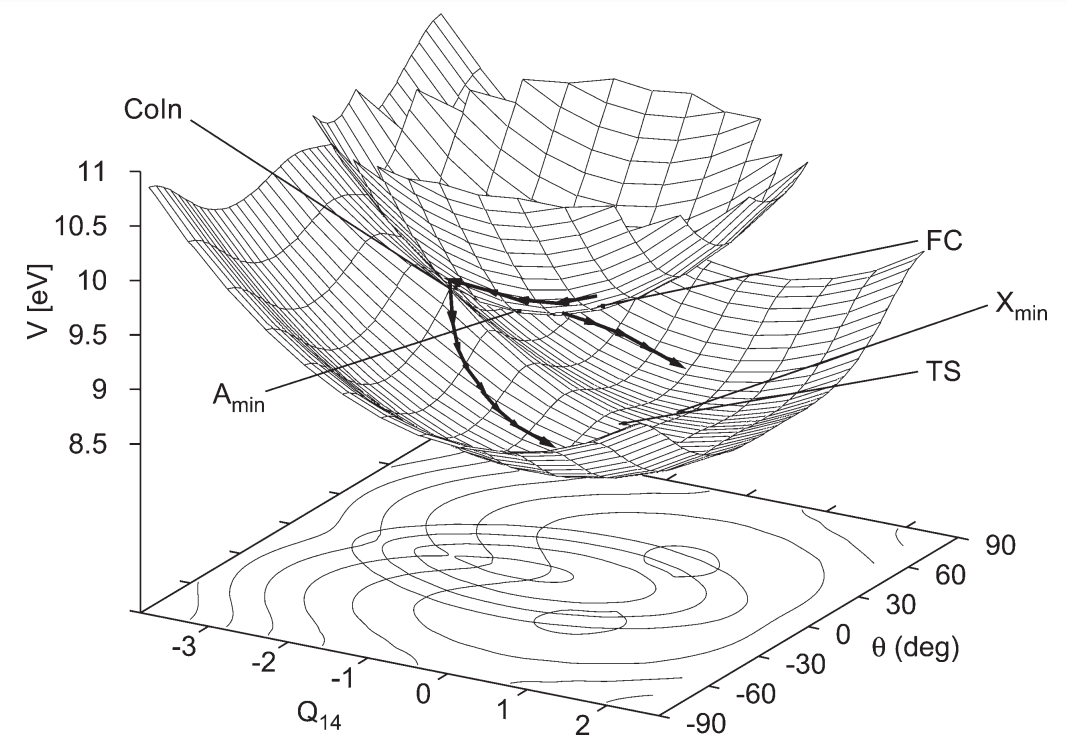
\includegraphics[width=\linewidth]{img/conical_intersection.png}
    \caption{3D surface plot of the conical intersection between two potential energy surfaces in the butatriene cation.\textsuperscript{\cite{directdynamics}}}
    \label{fig:conical_intersection}
\end{wrapfigure}

It is seen in the LHA (\ref{eq:lha}) that the first and second derivatives (gradient and Hessian) of the PES need to be defined. This may not be the case in the adiabatic scheme generated by the QC program where electronic states become degenerate (have the same energy) at particular points in the molecular configuration space.\textsuperscript{\cite{diabat}} This is known as a \textit{conical intersection} between the two potential energy surfaces (Fig.). At the intersection, the non-adiabatic coupling terms (NACT) between the two potential energy surfaces become infinite and the Born-Oppenheimer approximation breaks down.\textsuperscript{\cite{beyond}}

As such, the vMCG method must be run in the diabatic picture, where the corresponding PES is smooth. Transformations between the adiabatic and diabatic surfaces are also performed on-the-fly using a diabatisation scheme, which relies on a transformation matrix, \(\symbf{K}\). If we define the NACTs between adiabatic states \(\symit{ψ}_i\) with energy \(V_{ii}\) and \(\symit{ψ}_j\) with energy \(V_{jj}\) as
\begin{equation}
    F_{\symit{α},ij} = \frac{\bra{\symit{ψ}_i}\nabla_{\symit{α}}\hat{H}\ket{\symit{ψ}_j}}{V_{jj} - V_{ii}}
\end{equation}
where \(\nabla_{\symit{α}}\) is with respect to the coordinate \(R_{\symit{α}}\), then we can use the approximation
\begin{equation}
    \nabla\symbf{K} \approx -\symbf{F}\cdot\symbf{K} \label{eq:diabat}
\end{equation}
with \(\symbf{F}\) the matrix of NACT vectors. The equation is only exact if the basis set of electronic states is complete (infinite), which is not practical. Integrating (\ref{eq:diabat}) between two geometries at \(\symbfit{x}\) and \(\symbfit{x}+Δ\symbfit{x}\) gives the transformation matrix at the next step
\begin{equation}
    \symbf{K}(\symbfit{x}+Δ\symbfit{x}) = \exp\paren{-\int_{\symbfit{x}}^{\symbfit{x}+Δ\symbfit{x}}\symbf{F}(\symbfit{x}')\cdot\symup{d}\symbfit{x}'}\symbf{K}(\symbfit{x}),
\end{equation}
which concludes the scheme.\textsuperscript{\cite{diabat2}} In the \textit{Quantics} package, the QC database is implemented using \textit{SQLite}, where the tables for the diabatic gradient, Hessian, and PES are named \texttt{gra}, \texttt{hes}, and \texttt{pes} respectively, adiabatic data is stored in the \texttt{agra}, \texttt{ahes}, and \texttt{apes} tables, the NACT vectors in \texttt{nact}, and the adiabatic-to-diabatic transformation in \texttt{trans}.

\section{Design}\label{sec:design}

\subsection{Application programming interface}\label{ssec:api}

\begin{figure}[h]
    \centering
    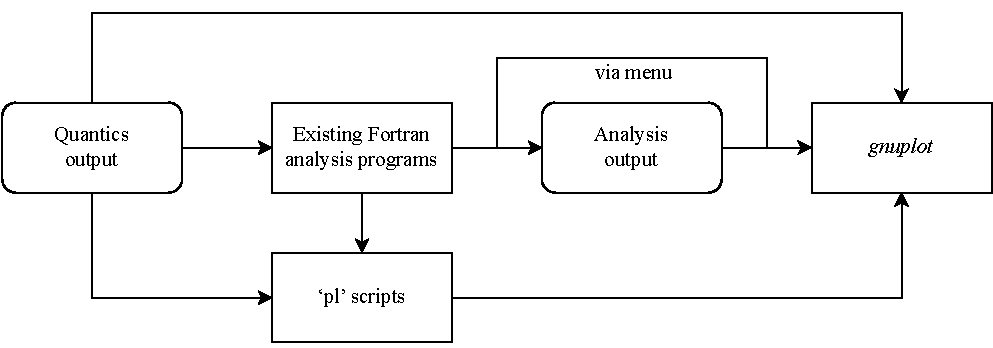
\includegraphics[page=1,width=0.8\textwidth]{img/old_api.pdf}
    \caption{Flow chart of dependencies for the currently implemented analysis system in \textit{Quantics}. Rounded boxes indicate files, and square boxes indicate programs.}
    \label{fig:old_api}
\end{figure}

In order to start to create a GUI we first need to find a way to connect to existing analysis programs written in Fortran. Figure \ref{fig:old_api} shows the analysis process currently implemented. The middle route is the method we used in \S\ref{ssec:butatriene} to plot the absorption spectrum with \texttt{autospec}: a Fortran program reads the output of a \textit{Quantics} simulation and outputs another file which can be read and plotted manually in \textit{gnuplot}.

Alternatively, if the Fortran program implements a menu, the program can directly call \textit{gnuplot} for plotting, without outputting any files. However, these menu programs offer an option to output the data used for plotting in a file for manual inspection of the data, which is particularly useful for our analysis GUI, as we generally do not want the analysis program to open a \textit{gnuplot} window when we call it.

The `pl'-scripts offer a different route. Depending on its purpose, the script calls a Fortran program and reads its file output, or reads the \textit{Quantics} simulation output directly, before calling \textit{gnuplot}. Finally, the top arrow indicates \textit{gnuplot} can also plot some of the simulation output directly.

The relationship between the analysis program and \textit{gnuplot} can be called an interface, specifically, an application programming interface (API).\textsuperscript{\cite{api}} \textit{Quantics} does not implement \textit{gnuplot}---it only uses it to visualise the file outputs of the analysis (or temporary file for `pl'-scripts and menu programs). Such is the basis of the analysis GUI. It can form an API to the existing Fortran programs through its file output. Thus, we can re-route Figure \ref{fig:old_api} as follows.

\begin{figure}[h]
    \centering
    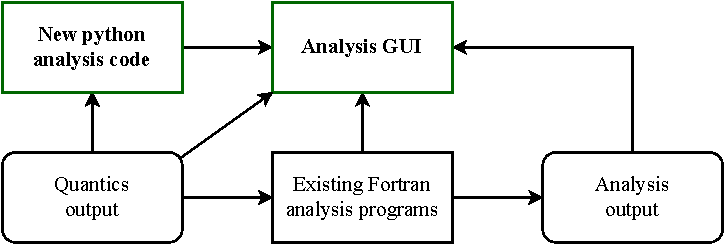
\includegraphics[page=1,width=0.6\textwidth]{img/new_api.pdf}
    \caption{Ideal analysis system for \textit{Quantics} using a GUI.}
    \label{fig:new_api}
\end{figure}

The analysis GUI can interface with the existing Fortran programs by calling it, similarly to the `pl'-scripts, then read and plot the output directly within the GUI. If the original \textit{Quantics} simulation output can be read directly, this can be implemented directly without an analysis routine being called. Lastly, as mentioned in \S\ref{ssec:aims}, the creation of new analysis code in Python can also interpret the \textit{Quantics} output and also can be fed into the GUI without using an intermediate file.

\subsection{User interface design}\label{ssec:ui_design}

The key to good user interface (UI) design is \textit{usability}.\textsuperscript{\cite{uid}} It is the extent a user can achieve their goals within the user interface based on three principles:
\begin{enumerate}
    \item \textit{Effectiveness}, how well a user can achieve their goals within the UI without running into errors, being lost, or needing help;
    \item \textit{Efficiency}, how much effort needs to be made in order to achieve the specified goals;
    \item \textit{Satisfaction}, how comfortable the user feels when interacting with the UI.\textsuperscript{\cite{iso}}
\end{enumerate}

In general, these are only factors to keep in mind when designing the UI, but can be quantified using a survey or questionnaire, which is talked about later in \S\ref{ssec:usability}. Before thse principles can be satisfied, however, we must understand what the goals mentioned in these principles are. For the purposes of the analysis GUI there are three tasks the user should be able to perform:
\begin{itemize}
    \item The user should be able to choose a directory, selecting a folder with the \textit{Quantics} output files;
    \item The user should see a list of analyses, choose an analysis and enter the parameters of the analysis;
    \item The user should visualise the analysis, either in text or in a graph/plot.
\end{itemize}

\begin{figure}[h]
    \centering
    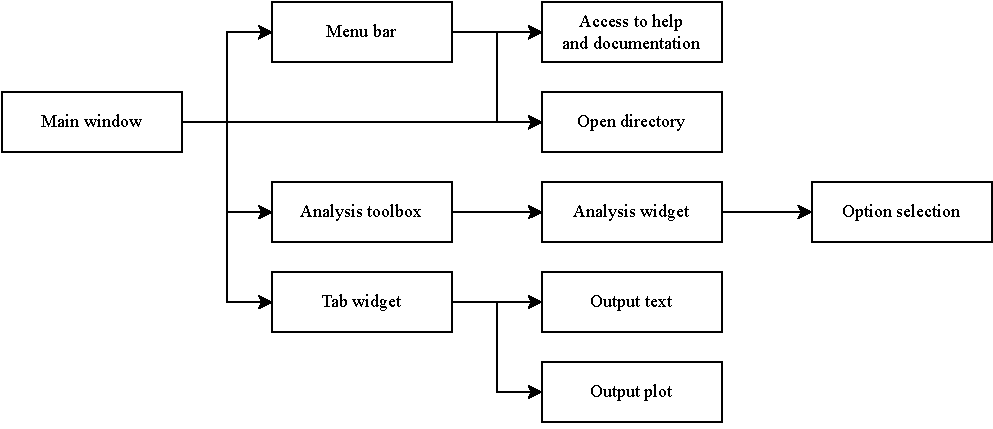
\includegraphics[page=1, width=0.7\textwidth]{img/content_diagram.pdf}
    \caption{A conceptional content diagram of the GUI.}
    \label{fig:content_diagram}
\end{figure}

To build a GUI around these tasks, it would be helpful to make a \textit{content diagram}, shown in Figure \ref{fig:content_diagram}. The second, third, and bottommost lines correspond to the three tasks just mentioned. Since an analysis output can be text-based or plot-based, we have a tab that can switch between the two. While it may be simpler to have one output view for both text and plot based analyses, the Fortran programs for plot-based analysis may also write a \texttt{.log} file or send additional information to the command line. This information can be written to the text widget for the user to view.

A secondary aim of the content diagram is to help in conceptual design, and allows the designer to see how usability can be maximised before working on the technical details. A number of heuristics exist for this purpose, though not all depend on solely the conceptual design. Some general principles that were kept in mind in creating Fig. \ref{fig:content_diagram} are:\textsuperscript{\cite{heuristics}}
\begin{itemize}
    \item \textbf{Consistency.} The directory can be written directly on the screen, which is the case for the \texttt{analysis} program, but also in the menu bar, which is consistent with many other GUIs.
    \item \textbf{Recognition, not recall.} An ``option selection'' box is included in the analysis widget which allows the user to select parameters for the analysis on the screen, rather than having to recall them.
    \item \textbf{Help and documentation.} In the menu bar, there should be a link to help and documentation on technical or less used aspects of the GUI, should they need it. Its implementation is explained in \S\ref{sec:doc_test}. However, it is also important that the design should allow the majority of users to achieve their goals without the use of further documentation.
\end{itemize}

To build a GUI using \textit{PyQt}, a user has two options. They can use code, or use \textit{Qt Designer}, a WYSIWYG (what you see is what you get) editor that allows elements of a GUI to be dragged directly where a person wants them. The use of Qt Designer also helps seperate the coding of the visuals itself from the coding of its implementation. As such, using \textit{Qt Designer} would be a better choice. In general, objects in Qt Designer fall in one of two categories:
\begin{itemize}
    \item \textbf{Composite widgets}, or containers, which may have other widgets inside of them. They can have a layout attached to them, which orders the subwidgets inside of them in a particular way (Horizontal, vertical, or a grid layout).
    \item \textbf{Input widgets}, which allows the system to obtain feedback from the user; for example, a \textit{text edit} can obtain a string from the user, a \textit{spinbox} can obtain an integer or a float, a \textit{checkbox} can obtain a boolean (true or false), and a \textit{combo box} or can obtain a choice from a number of predefined items.
\end{itemize}

Putting these widgets together, we can build something similar to Fig. \ref{fig:content_diagram} in Qt Designer.

\begin{figure}[h]
    \centering
    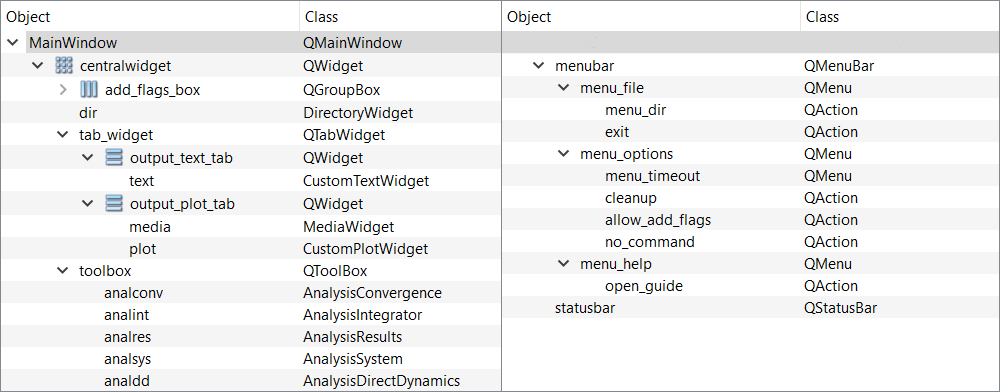
\includegraphics[width=0.7\textwidth]{img/content_diagram_designer.png}
    \caption{A tree view of contents as seen in the object inspector in Qt Designer.}
    \label{fig:content_diagram_designer}
\end{figure}

The main window is made of a central widget with a grid layout as indicated by the icon to the left of its name. The analysis options are categorised into the four main sections per listing \ref{lst:analysis_menu} (with the PES grouped with analyse system), as well as a fifth ``Analyse Direct Dynamics'' with new analyses explained in \S\ref{ssec:new_analysis}. The \texttt{MediaWidget} allows for control of animated plots (\S\ref{ssec:animated_plots}), and the contents of \texttt{add\_flags\_box} and \texttt{menu\_options} are also additional features discussed in \S\ref{ssec:additional_options}.

Some properties can also be set in Qt Designer, such as the margins or minimum size of a widget. A status tip property can be set on each analysis option, which displays a label on the status bar when hovering over it. This allows users familiar with the previous CLI-based analysis to know the name of the analysis program called by the GUI which they can consult the relevant part of the existing documentation.

\begin{figure}[h]
    \centering
    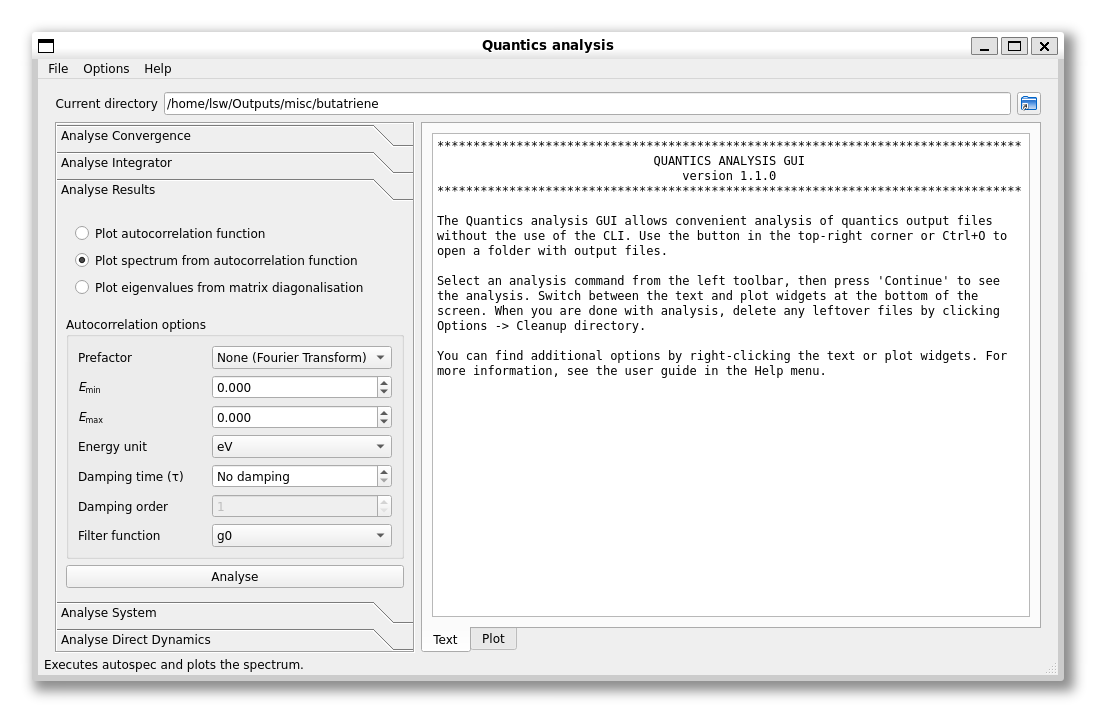
\includegraphics[width=0.7\textwidth]{img/analysis_gui.png}
    \caption{The analysis GUI as shown on startup.}
    \label{fig:analysis_gui}
\end{figure}

The final layout of the GUI is shown in Fig. \ref{fig:analysis_gui}. 
The design is meant to be simple and uncluttered, so that the important aspects of the GUI stand out more. The task for visualising the analysis the most important aspect of all the tasks, so it takes us the most space. At startup, no analysis can be visualised yet, so the GUI defaults to showing a concise description of what the GUI does.

Secondly, a list of analyses is shown of the left, seperated by the five categories mentioned above. Clicking each tab reveals a list of radio buttons, which correspond to the individual analyses. The user can input parameters for the analysis into the box below the radio button list. When the button `Analyse' is pressed, the analysis is performed and visualised in the text or plot widgets.

Finally, a short line dedicated to showing the current directory is shown at the top, below the menu bar.

\subsection{Object oriented programming}\label{ssec:oop}

Now that the design of the UI is complete, we need to add functionality to the GUI. In Qt and PyQt, this is done using signals and slots.
\begin{itemize}
    \item \textbf{Signals} are emitted when a widget on the screen is interacted with such that its internal state changes. When a signal is emitted depends on the widget and the interaction. For example, a button emits a signal when it is pressed, and a text edit emits a signal when its contents are modified, and a seperate signal if enter is pressed.
    \item \textbf{Slots} are the corresponding functions or methods that are executed when a signal is emitted. These functions are otherwise completely ordinary functions: nothing is special about them except that they are connected to a signal. The \mintinline{python}{@QtCore.pyqtSlot} decorator can be used to indicate that the method is a slot, but this is completely optional.
\end{itemize}

A signal and slots editor is present in Qt Designer but its functionality is severely limited: not all signals are available and slots can only take the shape of predefined functions. Thus, we have to use code to create slots and manually connect them to signals.

Objects in a GUI can naturally be represented by an object in a code, which are the underlying basis of object oriented programming (OOP). An object has attributes, or instance variables, which describe its internal state (e.g.~the current value in a spinbox), and methods, which are functions that have access to instance variables (e.g.~change the value in a spinbox).\textsuperscript{\cite{oop}}

The definition of an object is given by a class, which can be thought of as a template or blueprint of an object. We can import the UI file created by Qt Designer into a class representing the main window, which is called \texttt{AnalysisMain}, using the following code.
\begin{code}\begin{minted}{python}
from pathlib import Path
from PyQt5 import QtWidgets, uic
class AnalysisMain(QtWidgets.QMainWindow):
   def __init__(self):
      # call the inherited class' __init__ method
      super().__init__()
      # load the .ui file into the current class
      uic.loadUi(Path(__file__).parent/'main_window.ui', self)
\end{minted}
\caption{Code snippet for loading a UI file.}
\label{lst:pyqt_uic}
\end{code}
The use of the \texttt{Path} object allows the .ui file to be loaded from the Python file's directory. Otherwise, \texttt{uic.loadUi} tries to find it in the working directory that the user executes the Python file, which will likely not be the Python file's directory.

We can then place all the code/functionality of the GUI in this class. However, this is generally a bad idea because the resulting file will be very large in size, making organisation of the code and finding relevant methods or attributes harder, which in turn makes it harder to make modifications or add new features. Instead, we can split the code by responsibility, and have each class represent that responsibility. For example, the class \texttt{DirectoryWidget} has the single responsibility of storing and changing the directory that the GUI looks in to find output files. This is what is known as the \textit{single responsibility principle}, a key design principle in OOP.\textsuperscript{\cite{srp}}

These classes can then be interlinked using two well-known methods:
\begin{itemize}
    \item \textbf{Inheritance} allows the attributes and methods in a class, the parent class, to be used in another class, the child class, via inheritance. The child class can then add new attributes and methods which may use the parent class' attributes and methods.

    This is known as an ``is-a'' relationship; for example, the \texttt{QDialog} class handles a pop-up in a GUI to communicate with the user, like asking a question or as a notification. The \texttt{QFileDialog} class, used in \S\ref{ssec:dir_edit}, inherits from \texttt{QDialog}. It is also a pop-up, but specialises in asking the user to select a file or directory. Thus, a \texttt{QFileDialog} ``is a'' \texttt{QDialog}.
    \item \textbf{Composition} allows a child object to be an attribute of a parent object. The child object is contained within the parent class, and attributes and methods can be accessed and executed from the parent class.

    This is known as a ``has-a'' relationship; for example, a \texttt{QWidget} is a container than can have multiple \texttt{QRadioButton}s within it. Thus, the \texttt{QWidget} ``has a'' \texttt{QRadioButton} (or multiple of them). When a UI is loaded into a class via listing \ref{lst:pyqt_uic}, the attributes (child objects) are set automatically, and can be accessed via the object name in Qt Designer (Seen in Fig. \ref{fig:content_diagram_designer}).
\end{itemize}

These relationships can be visualised using a \textit{class diagram}. The class diagram of the analysis GUI is shown in Fig. \ref{fig:class_diagram}.

\begin{figure}[h]
    \centering
    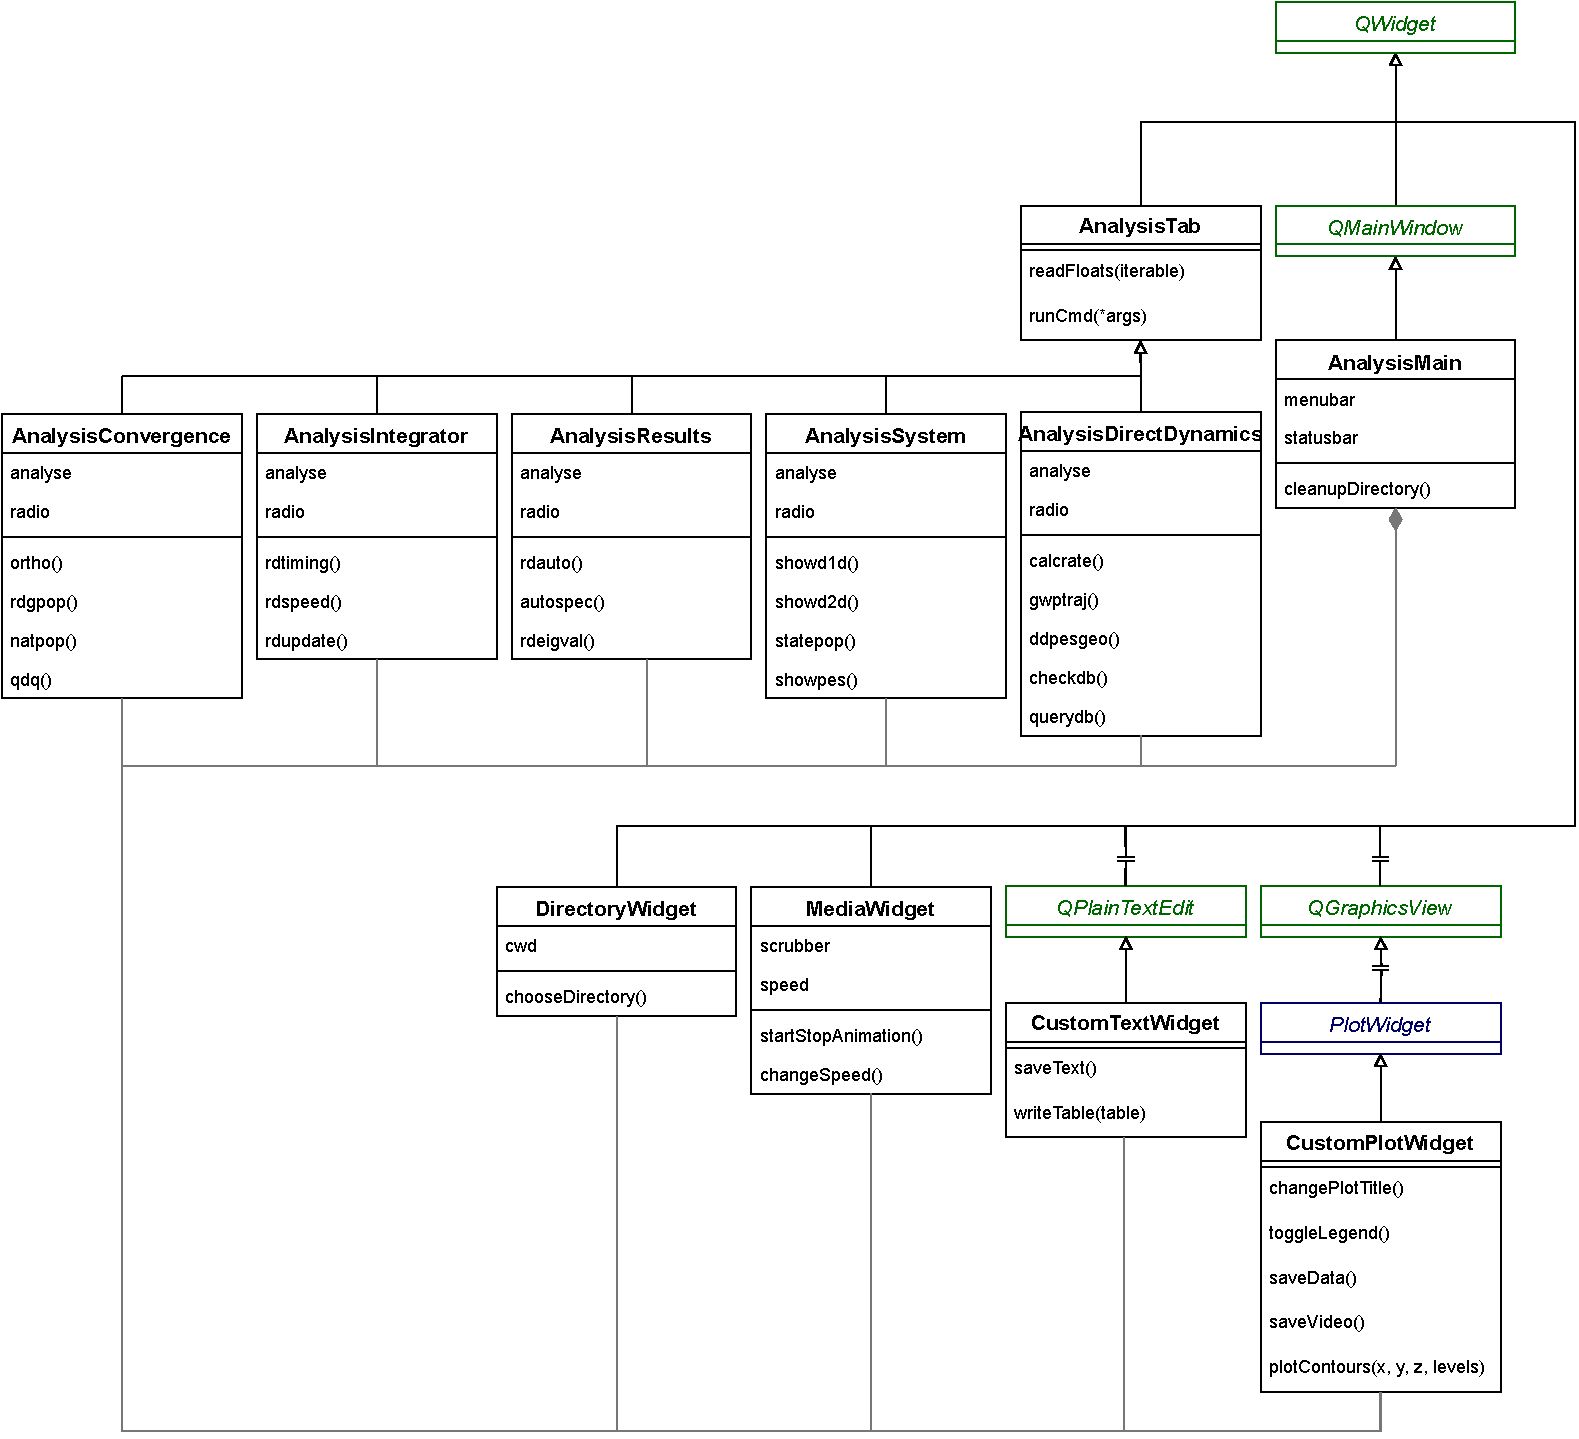
\includegraphics[page=1, width=\textwidth]{img/uml.pdf}
    \caption{Class diagram (UML specification) of the analysis GUI. Not all attributes and methods are shown. Green classes are implemented by \textit{PyQt}, the blue class by \textit{pyqtgraph}. The ``='' symbol means some layers of inheritance are hidden.}
    \label{fig:class_diagram}
\end{figure}

Each box represents a class. The first section has the name of the class, the second its attributes, and the third its methods. Inheritance is marked using an arrow with an triangular arrowhead from the child class to the parent class, and composition is marked using an arrow with a diamond arrowhead from the child object to the parent object. Section \S\ref{sec:implementation} details the implementation for each class.

There is one downside in not having all the code contained in one class, and it is that each promoted composite widget requires its own .ui file. Qt Designer only works with one .ui file at a time, and so it is not possible to see the contents of a composite promoted widget from the main window's .ui file, though multiple .ui files can be opened at the same time. This has the effect of making the UI design slightly harder to visualise.

\subsection{Packaging}\label{ssec:packaging}

In general, each file should only contain the details for one class, as this allows it to be easier to find the class for modification. These files can also be grouped into different folders depending on their purpose. In particular, the classes that perform analyses are placed in their own directory called \texttt{analysis/}, tests are placed in \texttt{tests/}, while the rest are placed in a directory called \texttt{ui/}.

\begin{code}\begin{minted}{text}
analysis_gui/
===============
ui/                ui/                                    
analysis/          ===============    analysis/             
tests/             __init__.py        ==================    tests/
__init__.py        main_window.py     __init__.py           ===========
gui.py             main_window.ui     convergence.py        fixtures/
environment.yml    dir_widget.py      convergence.ui        __init__.py
README.md          dir_widget.ui      integrator.py         run_tests.py
                   media_widget.py    integrator.ui         test_misc.py
                   media_widget.ui    results.py            test_analyses.py
                   analysis_tab.py    results.ui
                   custom_plot.py     system.py
                   custom_text.py     system.ui
                   coord_select.py    direct_dynamics.py
                                      direct_dynamics.ui
\end{minted}
\caption{Directories and files in the \texttt{analysis\_gui} folder.}
\label{lst:dir_files}
\end{code}

In order to allow classes in the folders to gain access to the contents of the other folder, we must make a \textit{Python package} by placing a file named \texttt{\_\_init\_\_.py} in each directory, as well as the directory above it. We can then use relative imports to obtain the classes in another folder. For example, in \texttt{analysis/convergence.py}, we can import the \texttt{AnalysisTab} class using \mintinline{python}{from ..ui.analysis_tab import AnalysisTab}, where the \texttt{..ui} looks for the folder \texttt{ui/} from one directory up.

Making a Python package also has a second purpose. In order to use inherited widgets in Qt Designer, you must ``promote'' the widget, by inserting the parent class into the GUI instead, then filling a form detailing the name of the child class and the location of the module (file) that the class can be imported from. For the latter, this can be made easier if all the files were located in a package. For example, using the directory structure in listing \ref{lst:dir_files}, the location of \texttt{convergence.py} can be specified as \texttt{analysis\_gui.analysis.convergence}.

Manual editing of the .ui files are required to conform with the schema in Fig. \ref{fig:class_diagram}. Firstly, promoted \texttt{QWidget}s are considered containers automatically by Qt Designer, which can be changed by manually removing \mintinline{xml}{<container>1</container>} from the \mintinline{xml}{<customwidgets>} section of the .ui file.

Secondly, it is not possible to promote the top-level widget in Qt Designer. In the .ui files in the \texttt{analysis/} directory, the top-level widget is required to be \texttt{AnalysisTab}, otherwise the \texttt{PyQt5.uic} module will complain that the class name is incorrect. To fix this, the \texttt{class} tag in the top-level widget can be changed manually in the .ui file, i.e.~from \mintinline{xml}{<widget class="QWidget">} to \mintinline{xml}{<widget class="AnalysisTab">}, assuming the \texttt{AnalysisTab} class is detailed in the \mintinline{xml}{<customwidgets>} section.

We can then create and open the GUI application as follows.
\pagebreak
\begin{code}\begin{minted}{python}
def openGui():
   app = QtWidgets.QApplication(sys.argv)
   # create and open the window
   window = AnalysisMain()
   window.show()
   # run the main Qt loop
   sys.exit(app.exec_())
\end{minted}
\caption{Code snippet of opening the main window using PyQt.}
\label{lst:open_gui}
\end{code}

This code is included in \texttt{gui.py}, but executing the code directly from this file will not work. This is because the \texttt{gui.py} file is inside the package, and Python does not consider the directory a Python file is executed in as a package (Python's creator, Guido van Rossum, considers this to be an ``anti-pattern'', i.e.~something to avoid\footnote{\url{https://mail.python.org/pipermail/python-3000/2007-April/006793.html}}). Thus all relative imports will fail. Instead, we can specify another file outside of the package (namely \texttt{quantics\_analysis\_gui.py}) which imports the \texttt{openGui} function of \texttt{gui.py} and runs it.

Finally, we must ensure the \texttt{analysis\_gui} package is located on \texttt{\$PYTHONPATH}, such that the \texttt{PyQt5.uic} module can find the package. This can be done by appending the folder location to the \texttt{sys.path} list. Once this is complete, it is possible to open the GUI from any Python file in any location using \mintinline{python}{from analysis_gui import gui} and \mintinline{python}{gui.openGui()}.

\subsection{Code style}\label{ssec:code_style}

The final design choice is the use of code style. In Python the use of the PEP8 style guide is encouraged.\textsuperscript{\cite{pep8}} However, the Python code makes large use of the PyQt package, which in general does not adhere to PEP8. If the code did use PEP8, this would make the code style inconsistent, which breaks the purpose of adhering to a style guide in the first place.

\begin{table}[h]
    \centering
    \begin{tabular}{@{}llll@{}}
    \toprule
    & \textbf{PEP8} & \textbf{PyQt/pyqtgraph} & \textbf{analysis\_gui} \\ \midrule
    \textbf{Attribute/Variable} & \texttt{snake\_case} & (\textit{inconsistent}) & \texttt{snake\_case} \\
    \textbf{Method/Function} & \texttt{snake\_case} & \texttt{camelCase} & \texttt{camelCase}\footnotemark \\
    \textbf{Class} & \texttt{PascalCase} & \texttt{PascalCase} & \texttt{PascalCase} \\
    \textbf{Module/File} & \texttt{snake\_case} & (\textit{inconsistent}) & \texttt{snake\_case} \\ \bottomrule
    \end{tabular}
    \caption{Code style recommendation for PEP8, Code styles used in PyQt/pyqtgraph, and code style chosen for \texttt{analysis\_gui}.\label{tab:code_style}}
\end{table}
\footnotetext{Except methods in the analysis widgets, which are named after the programs they call, making it easier to understand their purpose.}

Table \ref{tab:code_style} shows the format used in PEP8 and PyQt/pyqtgraph. The code for the analysis GUI uses the PyQt/pyqtgraph convention where possible, and PEP8 for all other cases.

\section{Implementation}\label{sec:implementation}

\subsection{Changing the directory}\label{ssec:dir_edit}

The first task is to embed a directory navigation widget into the GUI, so that the user knows what directory the analysis GUI is looking for output files in. This is done using the directory widget, which has an input widget \texttt{QLineEdit} for this purpose. This also allows the directory to be typed in by the user. At startup, the line edit is set to the current working directory using \texttt{Path.cwd()}.

\begin{figure}[h]
    \centering
    
\includegraphics[width=0.8\textwidth]{img/dir_widget.png}
    \caption{The directory widget as it appears in Qt Designer. The icon of the button cannot be set in Qt Designer so it appears blank; it is instead set in the code.}
    \label{fig:dir_widget}
\end{figure}

The goal of the widget is to provide the manipulation of the widgets' \texttt{cwd} attribute. This is a Path object that, for example, can be accessed by an analysis method to find an output file using \mintinline{python}{DirectoryWidget.cwd/'filename.txt'} (For Path objects, the forward slash appends to the path). Since the \texttt{QLineEdit} stores the directory, the \texttt{cwd} getter can simply return this text.

When the user enters a directory using the line edit, we can check that it is a valid directory by connecting the line edit's \texttt{editingFinished} signal to \texttt{cwd}'s setter that uses \texttt{Path.is\_dir} method. If it is not a valid directory, then we can revert to the previous valid directory by using \texttt{QLineEdit.undo()}, then display an error message using \texttt{QtWidgets.QMessageBox.critical}, which take the parent widget, title text, and message text as arguments (Fig. \ref{fig:dir_error}).

The second task is to allow the user to select a directory using a pop-up window, which can show the user's directory structure, activated by clicking on the button on the far right (or \texttt{Ctrl+O}/using the menu bar). PyQt has a widget for this purpose, known as \texttt{QtWidgets.QFileDialog}. To select a directory, we can use the \texttt{getExistingDirectory} method, which creates a new window per Fig. \ref{fig:dir_edit}. By default, this only shows the user's directories; it would be useful if it can show files as well, which can be done by passing it an empty options object \texttt{options=QtWidgets.QFileDialog.Options()} which overrides the default option \texttt{QtWidgets.QFileDialog.ShowDirsOnly}. Once the directory is selected, the new directory is passed to \texttt{cwd}'s setter.

\begin{figure}[h]
    \centering
    \begin{minipage}[t]{.47\textwidth}
        \centering
        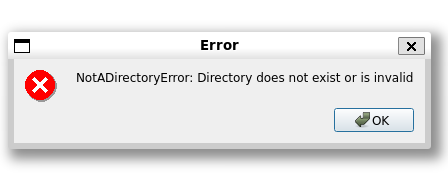
\includegraphics[width=\textwidth]{img/dir_error.png}
        \caption{Error popup from inputting an invalid directory.}
        \label{fig:dir_error}
    \end{minipage}\hfill\begin{minipage}[t]{.47\textwidth}
        \centering
        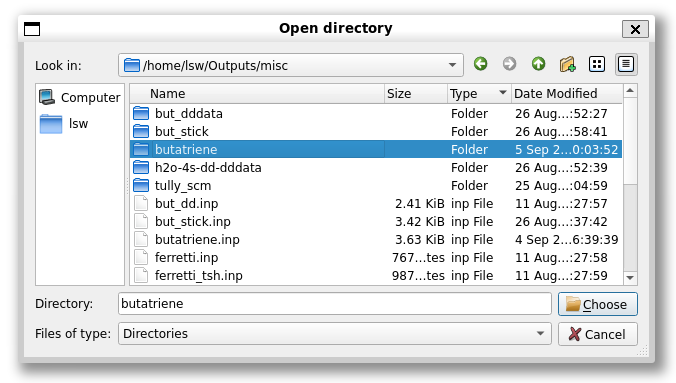
\includegraphics[width=\textwidth]{img/dir_edit.png}
        \caption{Dialog to select a directory.}
        \label{fig:dir_edit}
    \end{minipage}
\end{figure}

\subsection{The \texttt{AnalysisTab} widget}\label{ssec:analysistab}

The purpose of the \texttt{AnalysisTab} widget is to provide a framework that allows analysis methods to be implemented or created more easily. Each analysis tab (Fig. \ref{fig:analysis_gui}) inherits from this class (Fig. \ref{fig:class_diagram}) in order to obtain useful methods and have its basic functionality automatically implemented. Since each analysis tab shares many common features, this inheritance allows for code reuse.

In particular, each analysis tab shares common widgets: a list of radio buttons in a \texttt{QWidget} which represent a choice of which analysis to perform, and a push button \texttt{QPushButton} which performs the selected analysis. These widgets are created in Qt Designer and loaded into the inherited class in the class' constructor (the \texttt{\_\_init\_\_} method)

If we standardise the names of these widgets as \mintinline{python}{self.radio} and \mintinline{python}{self.analyse}, respectively, then basic signal-slot selection can be performed in the \texttt{AnalysisTab} class instead of manually for each inherited class. For example, if a mapping (dictionary) between the selected radio button's index and the method to execute when \texttt{analyse} is pressed is given in the inherited class, then the functionality of performing an analysis can be done using listing \ref{lst:analyse_pushed}.
\begin{code}\begin{minted}{python}
# in constructor, mapping defined between radio button index and method objects,
# e.g. self.methods = {0: self.analysisMethod0, 1: self.analysisMethod1}

# get index of checked radio button (there should only be 1)
radio_index = [index for index, radio in enumerate(self.radio) if radio.isChecked()][0]
# call method associated with index
self.methods[radio_index]()
\end{minted}
\caption{Code snippet of the \texttt{analysePushed} method.}
\label{lst:analyse_pushed}
\end{code}

However, a problem occurs if the button is pushed while an analysis is being performed. For analyses that take up more than a few seconds, clicking the button again will queue another method call in the system, i.e.~if the button is clicked twice, a redundant second method call will be performed. Ideally, the user should know the system is busy performing the analysis and the button should be frozen to prevent any further presses. This can be implemented using listing \ref{lst:freeze_analyse}. Note, the \texttt{repaint()} method needs to be called otherwise the button's status update is delayed until the next event loop, meaning that nothing happens---calling \texttt{repaint()} updates the button immediately.
\begin{figure}[h]
    \centering
    \begin{minipage}[b]{.57\textwidth}
        \begin{minted}{python}
QtWidgets.QApplication.setOverrideCursor(
    QtCore.Qt.WaitCursor # set cursor to 'wait'
)
self.analyse.setEnabled(False)
self.analyse.setText('Busy')
self.analyse.repaint()
# ... method call ...
QtWidgets.QApplication.restoreOverrideCursor()
self.analyse.setEnabled(True)
self.analyse.setText('Analyse')
        \end{minted}
        \captionof{listing}{Code snippet of freezing the push button until analysis is complete.}
        \label{lst:freeze_analyse}
    \end{minipage}\hfill\begin{minipage}[b]{.4\textwidth}
        \centering
        
\includegraphics[width=\textwidth]{img/busy.png}
        \caption{Top: The system is available to perform an analysis. Bottom: The system is busy performing an analysis. The cursor icons for both situations are also shown.}
        \label{fig:busy}
    \end{minipage}
\end{figure}

If the analysis method called raises an exception, the \texttt{analysePushed} method terminates early and the button will not unfreeze, preventing the user from doing anything. Therefore, the analysis method call is also wrapped in an try-except block, with the nature of the exception given to the user via \texttt{QtWidgets.QMessageBox.critical}. The complete traceback of the exception can then be given to the developer for debugging using
\mintinline{python}{print(traceback.format_exc(), file=sys.stderr)}.

\subsubsection{Checking a file exists}\label{sssec:check_file}

In addition to performing an action when \mintinline{python}{self.analyse} is pressed, we can also perform actions when a radio button in \mintinline{python}{self.radio} is pressed. This is useful since this allows us to change the state of the UI when a specific analysis option is selected. For example, most analyses require a certain output file to be present in the directory---if that file is not present, then we can disable \mintinline{python}{self.analyse} from being pressed.

Like the methods dictionary, these files can be given in the inherited class via a mapping, with a list of filenames in the current directory as the value. Firstly, we connect all the radio buttons to a slot method named \texttt{optionSelected} (Listing \ref{lst:check_file}), which for now only calls \texttt{checkFileExists}, but will have another purpose later (\S\ref{ssec:per_analysis}). Then, in the \texttt{checkFileExists} method, a list of missing filenames can be generated using a list comprehension \mintinline{python}{[file.name for file in filenames if not file.is_file()]}. If this list has any members, they are displayed on the frozen ``Analyse'' button (Fig. \ref{fig:missing_files}).

\begin{figure}[h]
    \centering
    \begin{minipage}[b]{.57\textwidth}
        \begin{minted}{python}
for index, radio in enumerate(self.radio):
    if radio.isChecked():
        self.checkFileExists(index)
        \end{minted}
        \captionof{listing}{Code snippet of the file checking functionality of the \texttt{optionSelected} method.}
        \label{lst:check_file}
    \end{minipage}\hfill\begin{minipage}[b]{.4\textwidth}
        \centering
        
\includegraphics[width=\textwidth]{img/missing_files.png}
        \caption{The ``Analyse'' button frozen, showing the missing files that are required for the chosen analysis.}
        \label{fig:missing_files}
    \end{minipage}
\end{figure}

\subsubsection{Reading values from a file}\label{sssec:read_floats}

The core method of interfacing with the Fortran analysis program is through the analysis output files. These files are often in the form of a grid of values (Listing \ref{lst:grid_floats}).

\begin{code}\begin{minted}{text}
0.00    3.0171885631E+02
1.00    2.8208406002E+01
2.00    3.0443131784E-03
3.00   -1.9018896319E+00
4.00   -1.6790777029E-01
\end{minted}
\caption{A grid of numbers produced from an analysis program. As an example, the first column might represent time, and the second might represent some other quantity.}
\label{lst:grid_floats}
\end{code}

It would be useful to implement a function which can read these files in \texttt{AnalysisTab} and produce a matrix of floating point numbers (a computer's representation of a real number) from it. A suitable data type for this would be a \textit{NumPy array}. \textit{NumPy} is a Python module that provides support for multi-dimensional arrays and mathematical functions to operate on these arrays.\textsuperscript{\cite{numpy}} The inherited classes' analysis methods can then plot this array, or manipulate it using NumPy's extensive library for scientific computing.

To create the NumPy array, it needs to be passed a list of lists: one representing rows, and one representing columns (or \(n\) nested lists for an \(n\)-dimensional array). Each row is located on a new line, so we can simply use a for loop to iterate over each line. Then for the cells in the rows, we can use \textit{regular expressions} (regex), which use a ``pattern'' to find sequences of characters which can then be turned into floats.

Initially, the code used a regular expression that only matches valid floating point number forms. The text would be converted to a float if and only if the text matches the float regex, such that we know the text-to-float parsing will succeed. This is known as a \textit{look before you leap} (LBYL) approach.

There is another approach in that we could use a regular expression that matched any sequence of characters (except whitespace). We do not know if text-to-float parsing will succeed, but if it does not, we can ignore that line. This is known as a \textit{easier to ask for forgiveness than permission} (EAFP), characterised by a try-except block over LBYL's \texttt{if} statement.\textsuperscript{\cite{eafp}} The code for both approaches is given in listing \ref{lst:read_floats}. Explanation for the regexes are given in \S\ref{ssec:regex}.

\begin{code}\begin{minted}{python}
def lbyl(iterable) -> np.ndarray:
    data = []
    regex = r'([+-]?\d+(?:\.\d*)?(?:[eE][+-]?\d+)?|\.\d+)'
    for line in iterable:
        matches = re.findall(regex, line)
        if matches:
            data.append(list(map(float, matches)))
    return np.array(data)

def eafp(iterable) -> np.ndarray:
    data = []
    regex = r'\S+'
    for line in iterable:
        matches = re.findall(regex, line)
        try:
            data.append(list(map(float, matches)))
        except ValueError:
            pass
    return np.array(data)
\end{minted}
\caption{LBYL and EAFP implementations of reading a grid of numbers. \texttt{iterable} can be a file object or a list of strings.}
\label{lst:read_floats}
\end{code}

Due to the relative complexity of the LBYL's float regex, it is assumed that the EAFP approach would be faster. To confirm this, the performance of both implementations were tested against a grid of \(4000\times 4\) floats, stored in a file. Each function parsed the file 1000 times. The time for the LBYL implementation was 21.69~s, while the EAFP implementation took only 14.59~s. As such, the EAFP approach was used in the code.

The \texttt{readFloats} method has a couple of additional optional parameters for flexibility. Firstly, if we expect that a file has a set number of columns, we can specify this in the \texttt{floats\_per\_line} parameter, such that if the format of the file has been updated, the code will fail on purpose, serving as an indicator to the developer to update the outdated code. This is also useful to prevent accidental errors with inhomogenous column lengths being parsed (e.g.~one row having two columns, the other having three). 

The second parameter is provide an optional ``ignore regex''. If a line matched this regex, the line would be ignored. This may be useful in a situation where the output files is in a \textit{gnuplot}-format where a \# symbol indicates a comment which should not be read. If the regex \mintinline{python}{r'^#'} is passed to this parameter, lines starting with \# will be ignored.

\subsection{The plot widget}\label{ssec:plot_widget}

To visualise analyses, a plot widget is implemented inside the GUI. This allows for a more native experience compared to something like \textit{gnuplot} which opens in a new window. In Python, the most popular package for plotting and visualisations is \textit{matplotlib}. However, \textit{pyqtgraph} was chosen to be the tool used to show plots and graphs since it integrates much more nicely with PyQt, and also has the advantages of being faster, more interactive, and providing a more understandable API leading to simpler code.

As an example of the last point, \textit{pyqtgraph} provides an interactive plot widget simply by adding \texttt{pyqtgraph.PlotWidget} as a component of the main window, while in \textit{matplotlib}, you must import \texttt{matplotlib.backends.backend\_qt5agg.FigureCanvasQTAgg} for the plot canvas, then \texttt{matplotlib.backends.backend\_qt5agg.NavigationToolbar2QT} to provide interactivity. However, \textit{matplotlib} is a much more comprehensive package with a lot more features; \textit{pyqtgraph} lacks certain abilities like contour plots which have to be implemented manually (see \S\ref{ssec:contour}).

The interactions the user can make with the plot widget implemented by default in \textit{pyqtgraph} are:
\begin{itemize}
    \item Ability to move the data on the screen by left-click and drag as well as zoom in on the data by right-click and drag or scroll wheel. User can also select ``one-button'' mode on the menu which allows the user to drag a box around the part of the graph they want to zoom into (Fig. \ref{fig:plot_drag}).
    \item Ability to show or hide each line in a multiline plot by clicking on the respective entry in the legend.
    \item Ability to perform built-in transformations to the data, such as \(\symup{d}y/\symup{d}x\), and conversion from linear plot to a log plot.
    \item Ability to export still images of the current plot as well as data in the plot as a .csv file (Fig. \ref{fig:plot_export}).
\end{itemize}

\begin{figure}[h]
    \centering
    \begin{minipage}[t]{.47\textwidth}
        \centering
        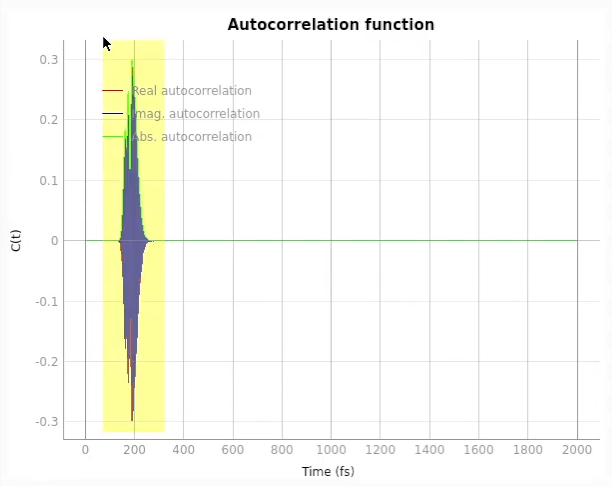
\includegraphics[width=\textwidth]{img/plot_drag.png}
        \caption{Dragging an area to zoom in on an interesting part of the plot in ``one-button'' mode.}
        \label{fig:plot_drag}
    \end{minipage}\hfill\begin{minipage}[t]{.47\textwidth}
        \centering
        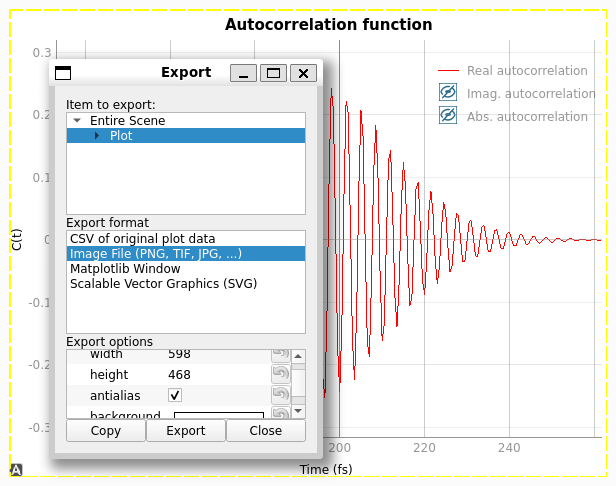
\includegraphics[width=\textwidth]{img/plot_export.png}
        \caption{Saving an image using \textit{pyqtgraph}'s built-in exporting option.}
        \label{fig:plot_export}
    \end{minipage}
\end{figure}

Analysis methods can call methods on the plot widget to create visualisations. However, the plot widget is a component of the main window, not a component of the analysis tab, so they must have a pointer to the main window to access the plot widget. This is given by PyQt using the \texttt{window()} method, such that the plot widget is accessed at \mintinline{python}{self.window().plot}, and the directory widget is accessed at \mintinline{python}{self.window().dir}.

To show a line plot using the plot widget, we simply use the \texttt{plot} method per \mintinline{python}{self.window().plot.plot(x_data, y_data, name=name, pen=pen)} where \texttt{x\_data} and \texttt{y\_data} are arrays, \texttt{name} is the corresponding label in the legend, and \texttt{pen} sets the style of the line, e.g.~\mintinline{python}{pen='r'} makes the line red.

If the user chooses to perform multiple analyses, the plot has to be refreshed to prepare for replotting. By inheriting from pyqtgraph's \texttt{PlotWidget}, we can add additional methods that may be helpful in the implementation of analysis methods, such as \texttt{reset()}, which clears the current plot and resets axis labels. This method will have additional purposes discussed later on.

We have now covered all the basic tools to create a basic analysis method. Assuming that we have created a .ui file, created a class for this .ui file that inherits from \texttt{AnalysisTab}, then adding the method name to \mintinline{python}{self.methods} and the required files to \mintinline{python}{self.required_files}, we can write something in the form of listing \ref{lst:generic_analysis}:

\begin{code}\begin{minted}{python}
def genericanalysis(self):
    filepath = self.window().dir.cwd/'filename'
    with open(filepath, mode='r', encoding='utf-8') as f:
        self.window().data = self.readFloats(f, floats_per_line=n_col)
    self.window().plot.reset(switch_to_plot=True)
    self.window().plot.setLabels(title='title', bottom='xlabel', left='ylabel')
    # repeat for each column...
    self.window().plot.plot(self.window().data[:, 0], self.window().data[:, 1],
                            name='name', pen='r')
\end{minted}
\caption{Code snippet of a generic analysis method that reads values from a file and plots them.}
\label{lst:generic_analysis}
\end{code}

This method looks for a file named \mintinline{python}{'filename'} in the user-selected directory and reads a grid of values with \texttt{n\_col} columns. We store the NumPy array returned from the \texttt{readFloats} method into an attribute in the main window because this allows us to more easily implement a method that can save this array to a user-defined location for future use (see \S\ref{ssec:customising}).

To plot the this array, we first clear any existing graph using \texttt{reset()}. Since there are two output tabs (one for text, one for the plot), we can automatically switch to the text tab using the \texttt{switch\_to\_plot} parameter, which simply calls \mintinline{python}{self.window().tab_widget.setCurrentIndex(1)} (The plot tab is at index 1). To plot the second column against the first column, we can use \textit{array slicing} in the form \mintinline{python}{self.window().data[rows_to_select, columns_to_select]} where a colon in \texttt{rows\_to\_select} selects all the rows.

The following subsections details specific variants of this basic code.

\subsubsection{\texttt{rdauto}}\label{sssec:rdauto}

If the keyword \texttt{auto} is given in the \textit{Quantics} input file, \textit{Quantics} will produce an \texttt{auto} file as an output. This file contains the \textit{autocorrelation function} \(C(t)\) defined as
\begin{equation}
    C(t) = \angled{\symit{Ψ}(0)|\symit{Ψ}(t)}
\end{equation}
which can be used to obtain the spectrum of a system (\S\ref{sssec:autospec}).

For symmetric Hamiltonians \(\hat{H} = \hat{H}^{\symsfup{T}}\) and real initial wavepackets \(\symit{Ψ}(0)\) we can use
\begin{equation}
    C(t) = \angled{\symit{Ψ}^*(t/2)|\symit{Ψ}(t/2)}
\end{equation}
which is generally more accurate and only requires propagation for half the time for which the autocorrelation function is necessary.\textsuperscript{\cite{auto}}

The format of the \texttt{auto} file is a grid of values with four columns, where the first column is time (in fs), and the second, third, and fourth columns are the real, imaginary, absolute values of the autocorrelation function at that time. When writing the code for this method, we can mention this a docstring, which is a description of what the code does. Listing \ref{lst:analysis_docstring} gives the docstring for the \texttt{rdauto} method.

\begin{code}\begin{minted}{python}
'''
Reads the auto file, which is expected to be in the format, where each cell is a float,

t.1    re.1    im.1    abs.1
t.2    re.2    im.2    abs.2
...    ...     ...     ...
t.m    re.m    im.m    abs.m

where t is time, and re, im, abs are the real, imaginary, and absolute value of the
autocorrelation function. Headers are ignored. Plots the autocorrelation function.
'''
\end{minted}
\caption{The docstring of the \texttt{rdauto} method.}
\label{lst:analysis_docstring}
\end{code}

Writing the docstring in this form allows future developers to know what format the file is expected to be in, allowing for easier debugging if the format of the file changes. Similar docstrings are present for all analysis methods covered in this report, but for conciseness only this one will be explicitly stated.

We can then use listing \ref{lst:generic_analysis} to implement the rest of this method, where the filename is \texttt{auto} and \texttt{n\_col} is 4. We can also set \mintinline{python}{ignore_regex='^#'} to ignore the header in the \texttt{auto} file. After setting the title and labels, we call \mintinline{python}{self.window().plot.plot} three times, plotting column 2, 3, 4 against column 1 for the real, imaginary, and absolute values of the autocorrelation function, respectively.

It may also be useful to the user if we write the contents of the auto file into the text widget for manual inspection. To do this we simply write \mintinline{python}{self.window().text.setPlainText(f.read())}, where \texttt{f} is the file object, followed by \texttt{f.seek(0)} such that \texttt{readFloats} can read the file from the beginning. Alternatively, for smaller files, we can set \texttt{txt = f.read()} and pass \mintinline{python}{txt.split('\n')} into \texttt{readFloats} instead.

\subsubsection{\texttt{rdspeed}}\label{sssec:rdspeed}

The \texttt{speed} file is created after a \textit{Quantics} simulation which reports the cumulative CPU and real time taken between each time step in the simulation. It has 6 columns: the propagation time (in fs), the CPU time (in seconds), the delta in CPU time (non-cumulative time between each time step), then the real time in a date format (\texttt{MMM DD hh:mm:ss}), in seconds, and in hours.

This format is slightly problematic for the \texttt{readFloats} methods due to the date column. Since the date contains text (specifically, for the month), parsing the file directly will fail since the method skips any lines that cannot be parsed into floats. The solution to this is simply to remove the date column using regex. We can match any date in the format \texttt{MMM DD hh:mm:ss} using \mintinline{python}{r'\w{3}\s+\d{1,2}\s+\d{2}:\d{2}:\d{2}'} (See \S\ref{ssec:regex} for an explanation) and replace them with blanks using \texttt{re.sub}. After this, the file can be parsed normally similarly to listing \ref{lst:generic_analysis}.

Only the CPU time and real time columns are plotted in this case, since the delta in CPU time can be retrieved using the in-built \(\symup{d}y/\symup{d}x\) transformation in the plot widget, and there is little point in plotting multiple lines for different units.

\subsubsection{\texttt{rdupdate}}\label{sssec:rdupdate}

For \textit{Quantics} simulations using a constant mean field (CMF) integrator (\S\ref{ssec:mctdh}) with an adaptive update interval, the \texttt{update} file is created. The basic idea behind CMF is that the matrix element \(\bra{\symit{Φ}_J}\hat{H}\ket{\symit{Φ}_L}\) and the inverse density matrix and mean field product \((\symbfit{ρ}^{(k)})^{-1}\angled{\symbf{H}}^{(k)}\) change much slower against time compared to the SPFs and the \(A\)-vector. Thus, they can be held constant for a longer propagation time, thus reducing computational cost, but not too long such that the error of SPFs and the \(A\)-vector passes a certain threshold.\textsuperscript{\cite{cmf}}

The update file contains five columns: the update step number, the update step size (time that the matrix element, etc. are held constant), the error of \(A\), the error of the SPFs, and the propagation time (cumulative step size). However, not every row has the same number of cells. If the error of either the coefficients or the SPFs passes a certain tolerance, the step is repeated with a smaller step size. The same happens if the integrator fails to converge. In these cases, only the step number is included in that row (possibly with the error as well).

The \texttt{floats\_per\_line} parameter in \texttt{readFloats} is useful for these failed steps. If we set this parameter to 5, then any failed steps are automatically ignored. We can then plot the update step size or the errors against the propagation time. However, since these represent different quantities we do not want to show all of them in one plot. We can let the user choose which quantity to plot using a combo box. This essentially acts as a parameter of the analysis method, and is further discussed in \S\ref{ssec:per_analysis}.

\subsubsection{\texttt{rdeigval}}\label{sssec:rdeigval}

\textit{Quantics} also contains methods for solving the time-independent Schr\"odinger equation, namely via the diagonalisation of the Hamiltonian, though it is not based on the MCTDH methods and only works for smaller systems. If the keyword \texttt{diagonalise} is given in the input file, the \texttt{eigval} file will be created containing the eigenvalues from the diagonalisation (column 2, in eV), as well as intensities (column 3), error estimates of the eigenvalues (column 4), and the excitations (column 6, in \(\symup{cm}^{-1}\)). The first column contains the number, and the fifth the eigenvalues in \(\symup{cm}^{-1}\), both of which are ignored. Like in \S\ref{sssec:rdupdate}, these are different quantities, and so the user chooses which column to plot using a combo box.

\subsection{Customising the plot and text widgets}\label{ssec:customising}

In the interactive CLI menus, options were available to the user to customise the aesthetics of the plot, such as toggling the visibility of the legend or the title (listing \ref{lst:showsys_menu}). Normally, this would not be possible by only using pyqtgraph's default \texttt{PlotWidget}, but we can inherit from this class to implement additional functionalities. We have already done this to implement a \texttt{reset} method in listing \ref{lst:generic_analysis}.

A suitable place for the user to change these settings are in the context menu, which can be made visible by right clicking on the widget. pyqtgraph has already some features in this menu such as transformations, manual setting of the \(x\) and \(y\) axes, grid visibility settings, etc.

To add options to these menus, we must acquire the underlying \texttt{QMenu} widgets. For the \texttt{PlotWidget}, the context menu is available at \texttt{PlotWidget.getPlotItem().vb.menu} and the ``Plot options'' submenu is available at \texttt{PlotWidget.getPlotItem().ctrlMenu} (See Fig. \ref{fig:plot_context_menu}). To add an option, we can use something like \mintinline{python}{self.action = menu.addAction('Option name')}. This returns a \texttt{QAction} object which has a \texttt{triggered} signal that can connect to a slot. This code can be placed in the constructor of the inherited \texttt{PlotWidget}, named \texttt{CustomPlotWidget}.

The most basic example of this is to add an option to show or hide the legend, shown in listing \ref{lst:context_menu}, which connects to a slot \texttt{toggleLegend} that, depending on whether \mintinline{python}{self.legend_checkbox.isChecked()} is \mintinline{python}{True}, shows or hides the legend using \texttt{show()} or \texttt{hide()}, respectively.

\begin{code}\begin{minted}{python}
plot_menu = self.getPlotItem().ctrlMenu
self.legend_checkbox = plot_menu.addAction('Show Legend')
self.legend_checkbox.setCheckable(True)
self.legend_checkbox.setChecked(True)
self.legend_checkbox.triggered.connect(self.toggleLegend)
\end{minted}
\caption{Adding a ``Show legend'' option into the context menu.}
\label{lst:context_menu}
\end{code}

The second customisation is to allow the user to change the title to one that they can specify. The user can then add additional information that the default title set in the analysis methods does not detail. To place a \texttt{QLineEdit} inside a menu, we create a \texttt{QWidgetAction} object and input the \texttt{QLineEdit} as a parameter to \texttt{QWidgetAction.setDefaultWidget}. The \texttt{QLineEdit.textChanged} signal can be connected to a slot that changes the plot title using \texttt{CustomPlotWidget.setTitle}. In order to add a label to the \texttt{QLineEdit} we can place it inside a submenu, which can simply be done using \texttt{QMenu}'s \texttt{addMenu} method, which returns another \texttt{QMenu} that can be used as shown above.

Note that using the method described above means that if the title is changed by the user, the original title set by the analysis method cannot be recovered. To fix this, we add an attribute named \texttt{default\_title} to \texttt{CustomPlotWidget} which can be changed by overriding (re-defining a method that already exists in the parent class) the \texttt{setLabels} method with the \texttt{title} parameter to change the \texttt{default\_title} attribute instead. The slot that changes the title can then check if the \texttt{QLineEdit} is empty, in which case the slot changes the title to \texttt{default\_title}---otherwise, the user-chosen title. If the user wants to clear the title completely, they can enter a empty space.

Though the intent of the GUI is to visualise analyses, it is not meant to create publication quality graphics. For users who need more customisation, touching up or modifying the results, we can also implement the ability to save the underlying NumPy array that the plot widget uses using \texttt{numpy.save}, which has the file's location and the NumPy array as parameters. While the in-built ``Export'' option can export an .csv of the currently plotted data, a NumPy array may be more convenient for Python users, and for animated plots (\S\ref{ssec:animated_plots}), the NumPy array will contain data for all frames rather than for the current frame only.

In the analysis method (listing \ref{lst:generic_analysis}) the NumPy array is stored at \mintinline{python}{self.window().data}. The user can then choose a file location using \texttt{QtWidgets.QFileDialog.getSaveFileName}, which brings up a window similar to Fig. \ref{fig:dir_edit}. If the user selects an existing file as a save location, NumPy will actually append the data to this file; to overwrite instead, we simply delete the file first. After the data is saved, the user is given a confirmation popup using \texttt{QtWidgets.QMessageBox.information} that communicates to the user that the data has been saved successfully.

\begin{figure}[h]
    \centering
    \begin{minipage}[t]{.47\textwidth}
        \centering
        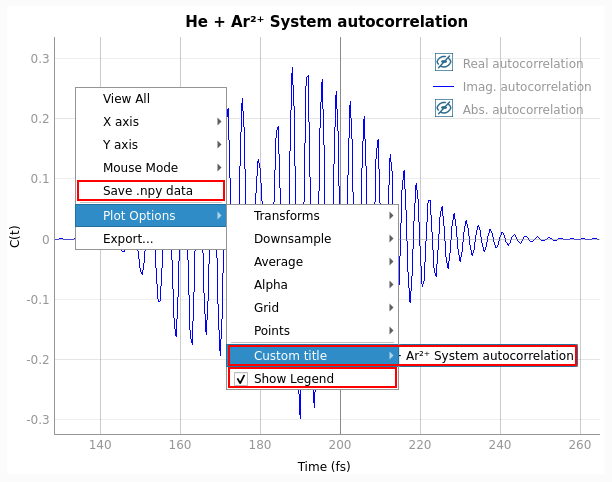
\includegraphics[width=\textwidth]{img/plot_context_menu.png}
        \caption{The context menu that appears when right-clicking on the plot widget. Additional options implemented highlighted in red. Not shown is the ``Save video'' option only visible for animated plots (\S\ref{ssec:animated_plots}).}
        \label{fig:plot_context_menu}
    \end{minipage}\hfill\begin{minipage}[t]{.47\textwidth}
        \centering
        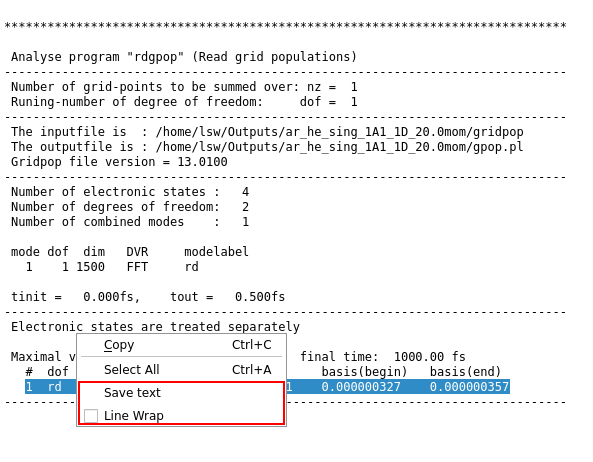
\includegraphics[width=\textwidth]{img/text_context_menu.png}
        \caption{The context menu that appears when right-clicking on the text widget. Additional options implemented highlighted in red.}
        \label{fig:text_context_menu}
    \end{minipage}
\end{figure}

In a similar vein, we can also inherit from \texttt{QPlainTextEdit} to provide additional features to the text widget. Adding extra options in the text widget context menu is slightly harder, however. First, the \texttt{contextMenuPolicy} attribute must be set to \texttt{CustomContextMenu}, which can be done in Qt Designer. This allows us to use the \texttt{customContextMenuRequested} signal, which we can connect to our own slot where we can add actions to the menu using the code in listing \ref{lst:text_show_menu}.

\begin{code}\begin{minted}{python}
def showTextMenu(self, point:QtCore.QPoint):
    text_menu = self.createStandardContextMenu(point)
    text_menu.exec_(text_menu.actions() + additional_actions, self.mapToGlobal(point))
\end{minted}
\caption{Code snippet to activate a custom menu in \texttt{CustomTextWidget}.}
\label{lst:text_show_menu}
\end{code}

We first create a \texttt{QMenu} using the \texttt{createStandardContextMenu} method. Then, to display this menu, the method \texttt{exec\_} is used, which takes in a list of actions and the \texttt{QPoint} (position) to show the menu in the program. We can thus specify any additional options in the \texttt{additional\_actions} list in listing \ref{lst:text_show_menu}. The \texttt{mapToGlobal} method is required to show the menu relative to the top-left corner of the main window rather than the top-left corner of the screen.

The extra options implemented in \texttt{CustomTextWidget} are a line wrapping toggling option, which if enabled breaks a long line that goes out of the screen to be displayed over multiple lines using the \texttt{setLineWrapMode} method, and a ``Save text'' option similar to the ``Save .npy data'' option except we can use the default Python text I/O methods to save the file. Text in the text widget is obtained using \texttt{toPlainText()}.

\subsection{Running commands using subprocess}\label{ssec:subprocess}

So far, we have written analyses for outputs directly from the \textit{Quantics} simulation. In order to interface directly with the Fortran analysis programs we can call them internally in the program. This can be done using Python's \texttt{subprocess} module simply using \texttt{subprocess.run(args)}, where \texttt{args} is a list of arguments, similar to calling the program on the CLI where a space seperates each argument. For example, the CLI command \texttt{autospec 9.0 10.5 ev 30 1} is equivalent to \mintinline{python}{subprocess.run(['autospec', '9.0', '10.5', 'ev', '30', '1'])}. However, doing it this way is not particularly useful as no feedback is returned on the status of the command line process executed. As such, it is useful to set number of optional arguments in the \texttt{subprocess.run} method.

Firstly, we must ensure the analysis program is called in the correct directory that the user specifies in the directory widget. This can be done setting the \texttt{cwd} parameter to \mintinline{python}{self.window().dir.cwd}. Secondly, in order to get feedback on the status of the program we must capture its output. In a command line interface, the text that the program outputs is known as the \textit{standard output} (\texttt{stdout}). Using the parameters  \texttt{stdout=subprocess.PIPE} and \mintinline{python}{text=True} allows the output to be ``piped'' (sent to) Python in text form (rather than a binary format), such that we can display it in the text widget using \mintinline{python}{self.window().text.setPlainText(p.stdout)} where \texttt{p} is the returned object from \texttt{subprocess.run}.

The program may also write to \textit{standard error} (\texttt{stderr}) if it encounters an error. This is also an output and can be combined with \texttt{stdout} using \texttt{stderr=subprocess.STDOUT}. Just because a program writes to \texttt{stderr} does not necessarily mean the program failed to work, however: this is instead communicated via the program's \textit{return code}. If the return code is 0, the program terminated successfully; for all other values, it had not. Setting the \texttt{check} parameter to \mintinline{python}{True} allows Python to raise an exception if the return code is non-zero. If these calls to the analysis programs are inside an \texttt{AnalysisTab} method, any exceptions raised will be communicated to the user (Fig. \ref{fig:subprocess_error}, also see \S\ref{ssec:analysistab} for implementation). However, due to bad programming practices in the Fortran code, calls to the analysis Fortran programs almost always return exit code 0 even if there are errors, with the exception of a couple of cases (e.g.~segmentation fault). This ends up causing problems with any analysis methods expecting a certain output from the command line process, causing it to return its own error (Fig. \ref{fig:subprocess_wrong_error}). This scenario is futher discussed in the limitations of the GUI (\S\ref{sssec:silent_errors}).

By default, the exception message raised by \texttt{subprocess.run} is not particularly useful as it only mentions the exit code of the process. The error message from the program is usually in its output which we can append to the exception message by catching it in a try-except block and re-raising the error with the appended message. Similarly, we can catch \texttt{FileNotFoundError}s, which are raised when the specified analysis program does not exist, to append the name of the missing program. To prevent having to do this for each subprocess call, there is a method called \texttt{runCmd} in \texttt{AnalysisTab} which does all of this well as set the optional parameters as specified above. There is one optional parameter, named \texttt{input}, which is passed to \texttt{subprocess.run} for analysis programs that require user input (such as \texttt{showsys}). The interface with menu-based CLI programs is discussed further in \S\ref{ssec:coordinate_selection}.

\begin{figure}[h]
    \centering
    \begin{minipage}[t]{.47\textwidth}
        \centering
        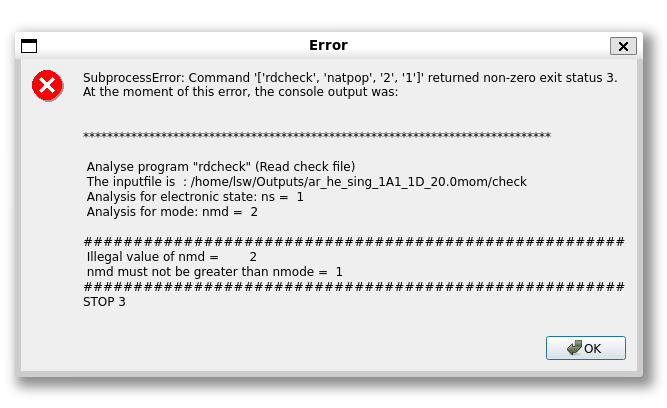
\includegraphics[width=\textwidth]{img/subprocess_error.png}
        \caption{The Fortran analysis program returns a non-zero exit code, and the error is successfully captured. Using the \texttt{runCmd} method allows \texttt{stdout} to be appended to the exception message.}
        \label{fig:subprocess_error}
    \end{minipage}\hfill\begin{minipage}[t]{.47\textwidth}
        \centering
        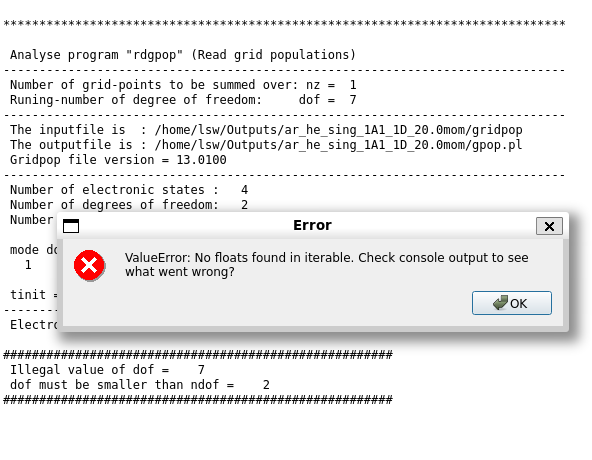
\includegraphics[width=\textwidth]{img/subprocess_wrong_error.png}
        \caption{The Fortran analysis program returns exit code 0 despite the fact that the program failed to run successfully. The explanatory error is seen in the output (text widget). In this case, it creates an empty file which \texttt{readFloats} fails to read---the error ``falls through'' to the next process.}
        \label{fig:subprocess_wrong_error}
    \end{minipage}
\end{figure}

\subsection{Per-analysis options}\label{ssec:per_analysis}

Most of the CLI analysis programs require additional parameters to control the nature of the output, and these parameters are different for each program. The user must specify these parameters before a call can be made to these programs. To implement this in the GUI, we can create a container full of input widgets in the .ui file, where each input widget adjusts the value of one parameter. In practice, some analysis programs contain so many optional parameters such that it may not be suitable to include them all inside the container. In this case, only the most important parameters can be changed using the input widgets---for any parameters not included, the GUI provides an alternative way to specify these (see \S\ref{ssec:additional_options}).

Each container is specific to one of the analyses (radio buttons), so a suitable choice of composite widget is \texttt{QGroupBox}, as shows a title above the container which we can write which analyses the container corresponds to. Fig. \ref{fig:autocol_box} and \ref{fig:clean_box} shows some examples of these \texttt{QGroupBox}es. 

\begin{figure}[h]
    \centering
    \begin{minipage}[t]{.47\textwidth}
        \centering
        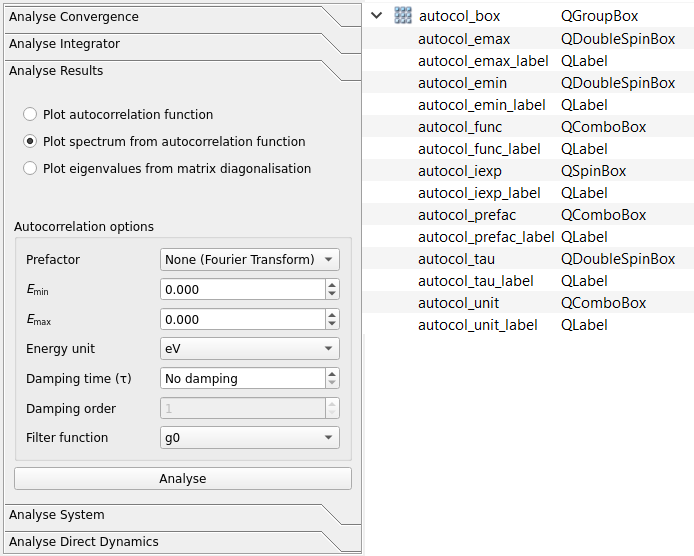
\includegraphics[width=\textwidth]{img/autocol_box.png}
        \caption{Left: the options container for the \texttt{autocol} analysis as it appears in the GUI. Right: the corresponding object list in Qt Designer.}
        \label{fig:autocol_box}
    \end{minipage}\hfill\begin{minipage}[t]{.47\textwidth}
        \centering
        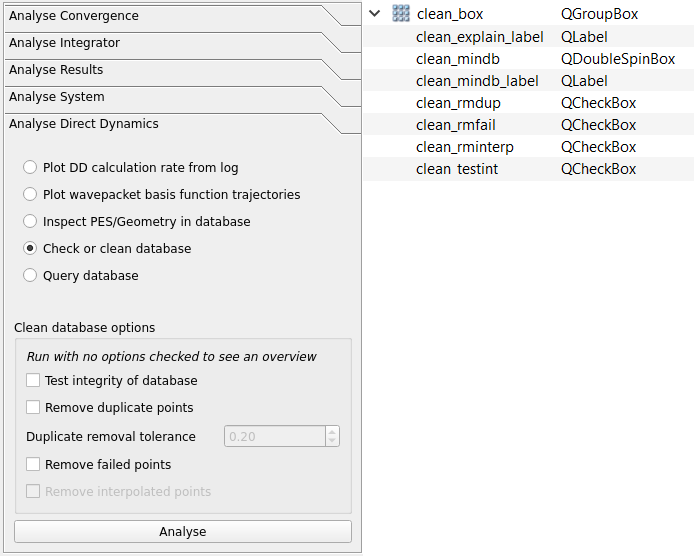
\includegraphics[width=\textwidth]{img/clean_box.png}
        \caption{Left: the options container for the \texttt{cleandb} program as it appears in the GUI. Right: the corresponding object list in Qt Designer.}
        \label{fig:clean_box}
    \end{minipage}
\end{figure}

We can then add a container show/hide feature to the \texttt{optionSelected} method in the analysis class. If the user passes another dictionary similar to \mintinline{python}{self.methods} or \mintinline{python}{self.required_files} (\S\ref{ssec:analysistab}), this time called \mintinline{python}{self.options} that contains the name of the container as the value, we can show the parameter container for the analysis that is selected, and only that analysis, using \mintinline{python}{self.options[index].show()}, and hide all other ones.

By loading the .ui file, the input widgets automatically become attributes of the analysis class, and their values can be directly obtained inside the analysis methods (e.g.~using \mintinline{python}{self.spinbox.value()}, \mintinline{python}{self.lineedit.text()}, etc.) without needing to add parameters to the function. In the previous sections \S\ref{sssec:rdupdate} and \S\ref{sssec:rdeigval} we mentioned how a combo box can be used to plot different columns. Using what we disscussed above, we can add a \texttt{QGroupBox} with a single combo box, then in the method a simple if statement of the form \mintinline{python}{self.combobox.currentIndex() == value} can be used to plot the user's choice.

The following subsections show examples of using these containers to change the parameters sent to the analysis call.

\subsubsection{\texttt{checkdb}}\label{sssec:checkdb}

The \texttt{checkdb} program is not as much of an analysis program as it is a convenience tool. No plotting is performed in this method; information that the program outputs is sent to the text widget. The main purpose of the program is to check the integrity of a QC database (\S\ref{ssec:ddvmcg}), but it also has the ability remove failed and duplicate entries. The task that it performs depends on the optional parameters it recieves. As such, it can be used to showcase the parameter container feature of the GUI.

The program will perform a task if it receives the corresponding flag. \texttt{-rd} reads the database to test its integrity, \texttt{-d} removes any duplicate points, \texttt{-c} removes any failed points, and \texttt{-sc} removes any failed or interpolated points. Each of these tasks can be represented as a checkbox in the GUI. Using a if statement for each checkbox, if the checkbox is checked (using \texttt{.isChecked()}), a string of the corresponding flag is added to a list of optional parameters, which is then sent to \texttt{runCmd}.

Since \texttt{-sc} is an extension of \texttt{-c}, it can be represented as two checkboxes: one for removing failed points, and one for interpolated points. We can then connect a signal that allows the interpolated points checkbox to be enabled only if the failed point checkbox is checked. Then, \texttt{-sc} is only added to the list of optional parameters if both the failed and interpolated checkboxes are checked. The code for the connection can be added to the constructor, and the decorator \mintinline{python}{@QtCore.pyqtSlot} can be used between analysis methods and slot methods in the analysis class.

By default, without any arguments, the program outputs an overview of the database properties, such as which tables are included, the total number of records (points), the number of atoms in the system, etc. To clarify this, a label is appended at the top of the container (see Fig. \ref{fig:clean_box}).

The final parameter included in the container is the duplicate removal tolerance, which is how close two points are to one another before they are considered duplicates. This is given the flag \texttt{-mindb f} where \texttt{f} is a float, so it is represented by a \texttt{QDoubleSpinBox} input widget (a \texttt{double} is a type of float). As a prerequisite, the flag \texttt{-d} must already be given. Like before, we can add a signal to enable the spinbox if and only if the duplicate checkbox is checked. The flag and the value of the spinbox can then be added to the list of optional parameters.

\subsubsection{\texttt{rdgpop}}\label{sssec:rdgpop}

For grid-based simulations, if the keyword \texttt{gridpop} is given in the \textit{Quantics} input file, a file with the populations of each grid point is given in the \texttt{gridpop} file. Unlike the \texttt{auto}, \texttt{speed} files covered in \S\ref{ssec:plot_widget}, this file is in a binary format and requires an external program to read, namely \texttt{rdgpop}. Reading the grid populations is one way to check the accuracy of a MCTDH calculation, as it can show whether enough basis functions have been used. It can also be used to see how much the grid can be made smaller, if there are any unpopulated grid points.

There are two mandatory, positional parameters to this function. The first is the number of grid points to sum over, named \texttt{nz}, and the second is the running number of DOFs to consider, named \texttt{ndof}. Both of these are integer values and can be represented by a \texttt{QSpinBox}. The \texttt{runCmd} method can then be called with the argument list \mintinline{python}{['rdgpop', '-w', str(self.gpop_nz.value()), str(self.gpop_dof.value())]}. The program outputs a file named \texttt{gpop.pl} which contains the time-evolution of the grid and basis points; the \texttt{-w} flag overwrites any existing files with the same name.

The \texttt{gpop.pl} file contains four columns: the start and end of the spacial grid populations, and the start and end of the basis occupations. This file can be read like normal using \texttt{readFloats} (akin to listing \ref{lst:generic_analysis}) and a line can be plotted for each column. The \texttt{stdout} output, written to the text widget, also contains the maximal values over all times, which may be more useful in some cases.

The plot widget's \texttt{pen} parameter in the \texttt{plot} method also allows different line types to be used, in addition to the colour of the line, if a dictionary is used instead. In particular, \mintinline{python}{{'color': 'b', 'style': QtCore.Qt.DashLine}} uses a dashed blue line. This style is used for the ``end'' columns, while the non-dashed lines are used for the ``start'' columns.

\subsubsection{\texttt{qdq}}\label{sssec:qdq}

The \texttt{check} file created after a \textit{Quantics} simulation contains various information on the properties of the wavefunction in the propagation, such as the norm, total energy, natural populations (\S\ref{sssec:natpop}), etc. It also contains data on the expectation values of the coordinate values, \(\angled{q}\), which can be interpreted as the trajectory of the wavepacket for that coordinate, and the standard deviation \(\angled{\symup{d}q} = \sqrt{\langle q^2\rangle - \langle q\rangle^2}\), which can be interpreted as the width of the wavepacket.

Like in \S\ref{sssec:rdgpop} the \texttt{check} file is in binary format and must be read using the \texttt{rdcheck} analysis program. Since multiple properties are stored in the \texttt{check} file it must know which quantities to retrieve using a parameter, which for this analysis method is \texttt{qdq}. The following two positional parameters specify the DOF \texttt{ndf} and the state \texttt{ns} to retrieve \(\angled{q}\) and \(\angled{\symup{d}q}\) from. The name of the output file is not fixed and depends on the positional parameters---it is of the form \texttt{qdq\_\{ndf\}\_\{ns\}.pl}. If parameters are stored in a list, the file name can be retrieved using an \(f\)-string \mintinline{python}|f'qdq_{"_".join(qdq_options)}.pl'|, which are a convenient way to use variables inside strings.

The output file contains three columns with time, \(\angled{q}\), and \(\angled{\symup{d}q}\), with the latter two being plotted against time.

\subsubsection{\texttt{autospec}}\label{sssec:autospec}

The absorption or photoelectron spectrum \(σ(\symit{ω})\) is proportional to the Fourier transform of the autocorrelation function \(C(t)\) previously mentioned in \S\ref{sssec:rdauto}. Specifically,\textsuperscript{\cite{autospec}}
\begin{equation}
    σ(\symit{ω}) = \frac{\symit{ω}}{2\symit{π}}\int_{-\infty}^\infty C(t)e^{i\symit{ω}t}\,\symup{d}t = \frac{\symit{ω}}{\symit{π}}\int_0^\infty \operatorname{Re}(C(t)e^{i\symit{ω}t})\,\symup{d}t \label{eq:spectrum}
\end{equation}

However, the integration up to \(t=\infty\) is impossible and therefore must end at some finite time \(T\). The actual equation used by the \texttt{autospec} program is
\begin{equation}
    \frac{1}{\symit{π}}\int_0^T \operatorname{Re}(C(t)e^{i\symit{ω}t})e^{-(t/\symit{τ})^{\symtt{iexp}}}g(t)\,\symup{d}t \label{eq:autospec}
\end{equation}
where the factor \(e^{-(t/\symit{τ})^{\symtt{iexp}}}\) allows the simulate the experimental line broadening and \(g(t)\) is a damping function to reduce the effect of the Gibbs phenomenon, which arises from the finite cutoff time. Note that the optional parameter \texttt{-EP} multiplies (\ref{eq:autospec}) by \(\symit{ω}\) to match (\ref{eq:spectrum}). By default, \texttt{autospec} is set to \texttt{-FT} without this multiplication. This choice of prefactor is given in the GUI.

There are five positional parameters required for \texttt{autospec}. The first three are the minimum, maximum, and unit of the energy to calculate the spectrum for. The first two are floats and can be represented by a \texttt{QDoubleSpinBox} in the GUI. The unit can be any choice of energy unit that is recognised by \textit{Quantics}, of which there are 11: namely, the electronvolt, Hartree (atomic units), nanometre wavelength, kcal/mol, kJ/mol, inverse electronvolt, Kelvin, Debye, megaelectronvolts, millihartrees, and attojoules. All 11 are included as a choice in a combo box.

The label of each item in the unit box does not correspond necessary with the position parameter's name in the GUI. For example, inverse electronvolts have the label \(\symup{eV}^{-1}\) but to use these units the parameter is \texttt{invev}. As such, the method defines a dictionary mapping the index of the combo box to the correct parameter name, such that the correct parameter can retrieved using \mintinline{python}{autocol_unit_map[self.autocol_unit.currentIndex()]}.

The last two parameters specify the damping time \(\symit{τ}\) and damping order \texttt{iexp}, respectively. Note that the value \(\symit{τ}=0\) is allowed and corresponds to removing the term involving \(\symit{τ}\) completely. To make this more obvious to the user, it is possible to set a special label in Qt Designer if the value is set to 0 which is set to ``No damping'' in this case (seen in Fig. \ref{fig:autocol_box}). Additionally, for \(\symit{τ}=0\) the \texttt{iexp} is not required and can be disabled in the GUI. We can use the damping time box's \texttt{valueChanged} signal to check if the damping time is set to 0, in which case the damping order box is disabled. Since the value 0 is ``falsy'', and all other values are ``truthy'', the slot can be implemented using a one liner: \mintinline{python}{self.autocol_iexp.setEnabled(bool(self.autocol_tau.value()))}. 

The output of the \texttt{autospec} program is to a file named \texttt{spectrum.pl}. Along with the energy in the first column, there are three other columns representing equation (\ref{eq:autospec}) with different damping functions \(g(t)\). By default, the columns correspond to \(g_0, g_1, g_2\) which are
\begin{equation}
    g_{n\in\{0,1,2\}}(t) = \cos^n\paren{\pi\frac{t}{2T}}. \label{eq:damping_functions}
\end{equation}
If the parameter \texttt{-lin} is input, the columns correspond to \(g_3, g_4, g_5\), where \(g_3\) is (\ref{eq:damping_functions}) with \(n=3\) and
\begin{equation}
    g_4(t) = 1 - \frac{t}{T}, \qquad \qquad g_5(t) = \paren{1 - \frac{t}{T}}\cos\paren{\frac{\symit{π}t}{T}} + \frac{1}{\symit{π}}\sin\paren{\frac{\symit{π}t}{T}}.
\end{equation}
All of these functions can be selected in the GUI. If the method ensures that \texttt{-lin} is set for \(g_{n>2}\) then the correct column can be selected using the slice \texttt{[:, i\%3+1]} for \mintinline{python}{i=self.autocol_func.currentIndex()}.

\subsection{Plotting a variable number of lines}\label{ssec:variable}

In this section, we will discuss analysis methods where the number of columns are not fixed, such that the \texttt{floats\_per\_line} parameter cannot be specified. This might happen, for example, where there is a column for a quantity for each state. One can use a simple for loop in this case.
\begin{code}\begin{minted}{python}
from pyqtgraph import intColor as colr
# ...
for i in range(n_cols-1):
self.window().plot.plot(self.window().data[:, 0], self.window().data[:, i],
                        name=f'col {i}', pen=colr(i, n_cols-1, maxValue=200))
\end{minted}
\caption{Using a for loop to plot a variable number of lines.}
\label{lst:colr}
\end{code}

A unique colour is used for each line to differentiate between lines. This is done using pyqtgraph's \texttt{intColor} method, which we specify the index and the number of hues. If we specify the number of hues as the number of columns (minus the column used for \(x\)), then \texttt{intColor} will automatically step through a collection of colour values evenly split across the colour spectrum, which can end up making a rainbow effect (see Fig. \ref{fig:natpop}). The \texttt{maxValue} specifies the brightness, which is made slightly darker than the default value to contrast against the white background.

\begin{figure}[h]
    \centering
    \begin{minipage}[t]{.47\textwidth}
        \centering
        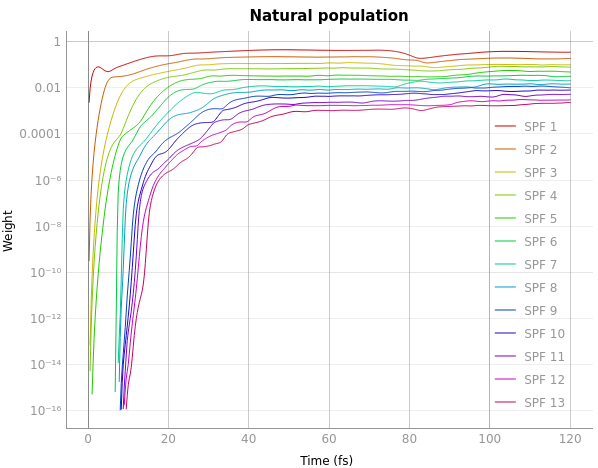
\includegraphics[width=\textwidth]{img/natpop.png}
        \caption{Example of a \texttt{natpop} output. A line is plotted for each SPF.}
        \label{fig:natpop}
    \end{minipage}\hfill\begin{minipage}[t]{.47\textwidth}
        \centering
        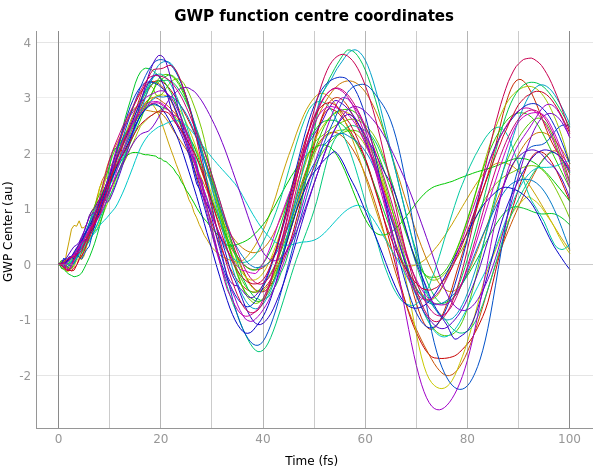
\includegraphics[width=\textwidth]{img/gwptraj.png}
        \caption{Example of a \texttt{gwptraj} output. A line is plotted for each GWP, of which there are 30. The legend is not shown for this analysis.}
        \label{fig:gwptraj}
    \end{minipage}
\end{figure}

\subsubsection{\texttt{natpop}}\label{sssec:natpop}

The natural populations were previously mentioned in \S\ref{ssec:mctdh}. They indicate the convergence of the MCTDH calculation. This data is stored in the \texttt{check} file, similarly to \texttt{qdq} (\S\ref{sssec:qdq}), for which the corresponding analysis program is \texttt{rdcheck}, this time with the \texttt{natpop} parameter.

After specifying the mode \texttt{nmd} and state \texttt{ns} the time-evolution for each SPF in the mode is given in the output file with form \texttt{natpop\_\{nmd\}\_\{ns\}.pl}. There is one column for time and one column for each SPF, which can be read using \texttt{readFloats} and them plotted using a for loop per listing \ref{lst:colr}. The standard output (in the text widget) also contains information of the maximum populations over all times for each mode and state, which may also be useful for the user.

\subsubsection{\texttt{statepop}}\label{sssec:statepop}

For systems with more than one electronic state, the diabatic state populations may be of interest to the user. In the \texttt{input} file, electronic states can be specified in a \textit{single-set formulation}, where they are represented as a single DOF where the number of SPFs are set to the number of states, or in a \textit{multiset formulation}, where different sets of SPFs are used for each electronic state: here, the wavefunction is expanded per
\begin{equation}
    \ket{\symit{Ψ}} = \sum_{\symit{α}}\symit{Ψ}^{(\symit{α})}\ket{\symit{α}}
\end{equation}
where, for MCTDH calculations, each state function \(\symit{Ψ}^{(\symit{α})}\) is expanded in MCTDH form.

For the MCTDH single-set formulation, the state population is given in the density matrix of the electronic DOF \(p_{\symit{α}}(t) = \symit{ρ}_{\symit{αα}}(t)\), while for the multiset formulation it is given using the norm \(||\symit{Ψ}^{(\symit{α})}||^2\).\textsuperscript{\cite{mctdh}} These populations can be retrieved from the \texttt{check} file using the program \texttt{statepop}. There is also \texttt{rdcheck spop} which performs an identical task---the choice of which to use is completely arbitary. No parameters are required for either choice.

The output file for \texttt{statepop} is to a file named \texttt{spops} containing a time column and one column for each state. The time-evolution of the state population is plotted for each state over \mintinline{python}{range(1, n_states + 1)}.

\subsubsection{\texttt{ortho}}\label{sssec:ortho}

The program \texttt{ortho} calculates the orthonormality errors of the SPFs. It can be used in conjunction with \texttt{norm} to ensure that the norm of the wavefunction remains constant throughout the simulation. However, the \texttt{norm} analysis program is currently broken and cannot be interfaced with at the time of writing this dissertation.

No output to a file is made for \texttt{ortho}. The output is instead made to \texttt{stdout}. This output is rather problematic for \texttt{readFloats} as it also contains other information such as the directory of the file, a list of mode labels, etc. If there are any floats in this other information the conversion to a NumPy array will fail. As such, we must read only the grid of values using by selecting the relevant part using regular expressions. This is made convenient as the grid of values are preceded and succeeded by the column headers, which start with \#. Using the regex \mintinline{python}{r'#.*?\n(.*)#'} with the \texttt{DOTALL} flag, any text between these headers are selected (see \S\ref{ssec:regex} for explanation).

There are always three columns in the output: the time, state, and the total orthonormality error. The rest of the columns detail the orthonormality error for each mode. For simulations with multiple states the state column will loop through all the states at each time interval, which essentially makes the data a three-dimensional array with time, mode, and state as the axes. To make plotting easier, the user chooses the state to inspect using the parameter container, such that a multiline plot with a line representing each mode can be used.

To select only the rows corresponding to the user's selection of state, a NumPy mask can be used in the form \mintinline{python}{self.window().data[self.window().data[:, 1] == state, :]}, where the slice \texttt{[:, 1]} selects the state column. If the returned data is empty we can conclude that the user selected an invalid state and an exception is raised. The plotting then proceeds as normal, with each mode being plotted as a seperate line along with the total orthonormality error.

\subsubsection{\texttt{gwptraj}}\label{sssec:gwptraj}

For methods using a GWP basis, such as G-MCTDH or vMCG, the trajectories of the centres of each wavepacket can be plotted along a certain mode in position space or momentum space using \texttt{gwptraj}. It is normally used as a menu-based program, but using the \texttt{-trj} flag, the programs leaves an output file named \texttt{trajectory} containing all the trajectories before exiting. A log file, which may contain some useful information to the user, is also created and can be appended manually to the text widget by opening it and using the \mintinline{python}{self.text.appendPlainText} method.

For the \texttt{trajectory} file, \texttt{gwptraj} writes a column for time and then, for each GWP, writes a column for each mode. For example, if there are 20 GWPs and 10 modes, the first 10 columns after the time column would be for the first GWP's trajectory for each of the 10 modes, then the second, etc. for a total of 201 columns. \texttt{gwptraj} then repeats this for the GWP momenta, for a total of 401 columns.

A visualisation of interest is the trajectory of each GWP along a single mode. If the user wants to look at the GWP centres and specifies the mode to inspect as \(m\), the indices of the correct columns to plot are \(m+1, m+n_m+1, m+2n_m+1, \dots, m+n_{\text{gwp}}n_m+1\) where \(n_m\) is the number of modes and \(n_{\text{gwp}}\) is the number of GWPs. If the user wants to look at the GWP momenta an offset of \((n_{\text{col}}-1)/2\) must be added to \(m\). This can be done using a for loop over \mintinline{python}{range(offset, offset+ngwp*nmode, nmode)} where the third parameter is the step value or number to increment.

Therefore, we must know either \(n_m\) or \(n_{\text{gwp}}\) to implement this successfully (the other can be calculated from the number of columns). Unfortunately, the \texttt{trajectory} does not contain this information by having a ``GWP'' or ``Mode'' column (like the ``State'' column in \S\ref{sssec:ortho}), but the \texttt{input} file does, where the number of GWPs is stated using \texttt{ngwp = i}. This can be selected using the regular expression \mintinline{python}{r'ngwp\s*?=\s*?(\d+)'} where \texttt{\textbackslash{}s*?} represents any possible number of whitespace before and after the \texttt{=} sign. In the unlikely event that \texttt{ngwp} is not stated or the input file cannot be found, the user is asked to input \texttt{ngwp} manually in a popup using \texttt{QtWidgets.QInputDialog.getInt}.

\subsection{Bar charts}\label{ssec:bar}

Categorical data can be visualised using a bar chart instead of a line plot. In pyqtgraph, bar charts can be plotted with a \texttt{BarGraphItem}, which can be appended to the plot widget using \texttt{addItem}. The parameters for \texttt{BarGraphItem} depends on the orientation of the bar chart. For horizontal bar charts, \texttt{x} specifies the positions and \texttt{height} is set to the values, while in vertical bar charts the extra parameter \texttt{y0=0} is required to specify the orientation, then \texttt{y} specifies the positions and \texttt{width} is set to the values. Unlike in \textit{matplotlib}, pyqtgraph does not have the ability to rotate axis tick labels, meaning a vertical orientation is more suitable for plotting categorical data with long labels while the horizontal orientation is more suitable for histograms (See Fig. \ref{fig:timing_bar} and \ref{fig:timing_bar_wrong}).

\begin{figure}[h]
    \centering
    \begin{minipage}[t]{.47\textwidth}
        \centering
        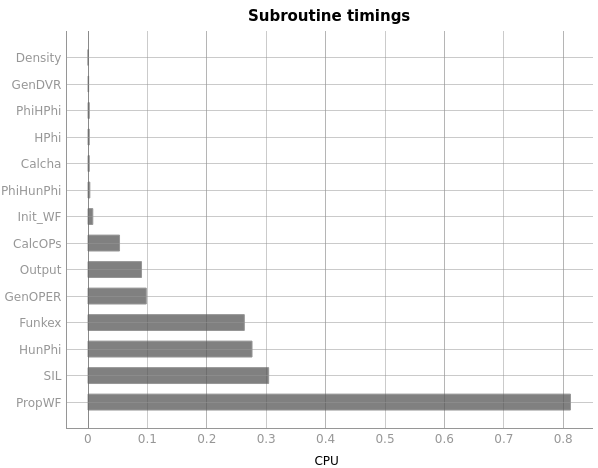
\includegraphics[width=\textwidth]{img/timing_bar.png}
        \caption{Example of a bar chart visualisation performed in \texttt{rdtiming}.}
        \label{fig:timing_bar}
    \end{minipage}\hfill\begin{minipage}[t]{.47\textwidth}
        \centering
        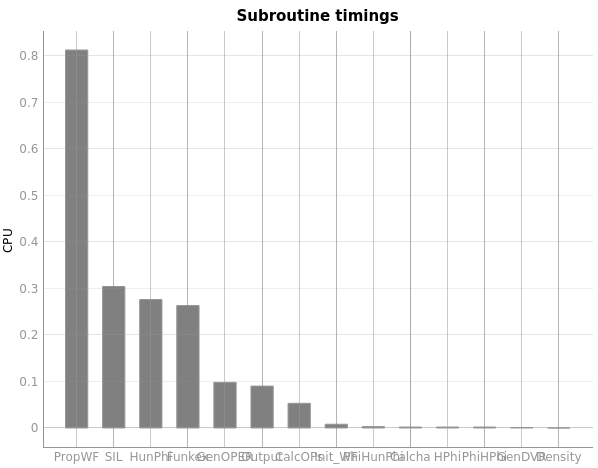
\includegraphics[width=\textwidth]{img/timing_bar_wrong.png}
        \caption{\texttt{rdtiming} with horizontal orientation. The tick labels cannot be rotated so this format is unsuitable.}
        \label{fig:timing_bar_wrong}
    \end{minipage}
\end{figure}

To specify custom tick labels in pyqtgraph, a list of list of tuples must be provided in \texttt{AxisItem.setTicks} where the \texttt{AxisItem} can be retrieved in the GUI, say for the for the \(y\) axis, via \mintinline{python}{self.window().plot.getAxis('left')}. Each tuple contains the position of the tick, and the label string. The list of lists has two lists which correspond to major ticks and minor ticks, respectively. Listing \ref{lst:tick_labels} contains the code to set the major ticks of a bar chart given a list of positions \texttt{positions} and a list of labels \texttt{labels}.

\begin{code}\begin{minted}{python}
ticks = []
for i, label in enumerate(names):
    ticks.append((positions[i], label))
self.window().plot.getAxis('left').setTicks([ticks])
\end{minted}
\caption{Setting custom tick labels in pyqtgraph.}
\label{lst:tick_labels}
\end{code}

\subsubsection{\texttt{rdtiming}}\label{sssec:rdtiming}

The \texttt{timing} file is created after a \textit{Quantics} simulation containing the time spent by the computer in each subroutine (function) and the number of times it is called. This can be used to increase the efficiency of a simulation; for example, it can tell the percentage of CPU time that is spent propagating the SPFs. If this percentage is too low or too large, one may consider combining or un-combining modes (\S\ref{ssec:mlmctdh}).

The \texttt{timing} file contains a column containing the subroutine name and then columns for the number of calls, the CPU time per call, the total CPU time, the percentage of total CPU time spent, and the total clock time. The method \texttt{rdtiming} reads this \texttt{timing} file and performs two tasks. Given a user selection of column in a combo box \texttt{timing\_sort}, the method sorts the timing file for that column and then plots a bar chart (e.g.~Fig.\ref{fig:timing_bar}). 

To do this, the information in \texttt{timing} must be parsed. Unfortunately, as the subroutine name is a string the \texttt{readFloats} method is unable to read this file. Therefore a special implementation must be used. Firstly, the \texttt{timing} file also contains miscellaneous information before and after the grid of subroutine data (such as host/device name, current date and time, and directory). We use regular expressions to split the file into three parts: miscellaneous data before the subroutine data (\texttt{pre}), the subroutine data, and the miscellaneous data after (\texttt{post}), using \mintinline{python}{r'(?<=Clock)\n|\n(?=Total)'} where ``Clock'' is the word before the data and ``Total'' is the next word after the data (see \ref{ssec:regex} for explanation).

Secondly, the subroutine data is loaded into a table by finding all sequences of characters seperated by whitespace using the regex \mintinline{python}{r'\S+'} (identical to the EAFP in \S\ref{sssec:read_floats}) in each line. Note a NumPy array is not suitable format for the table as one column contains strings (\texttt{numpy.save} still works despite this). However, as the subroutine name may contain spaces, this may make the subroutine name take up more than one entry, but as we know there are 6 columns the leftmost entries can be combined if the length of the row is larger than 6. A final column is added to the column that contains the entire line as a string: this saves having to re-format the data after sorting.

To sort the data, we can use the in-built Python function \texttt{sort} with the key parameter specified, which is a function to sort the list by. The key \mintinline{python}{lambda x: -x[self.timing_sort.currentIndex()]} automatically sorts using the user's specified column. The minus sign reverses the order such that the largest values come first. Note if the user selects the subroutine name as the sort, the minus sign is omitted such that it sorts A--Z. The \texttt{timing} file can then be recreated with the sort by using the \texttt{pre},  \texttt{post}, and the final column of the sorted table.

A bar chart can then be plotted in the same way as described in \S\ref{ssec:bar}. Note if the user selects subroutine name as the column the values of the bar default to the CPU time.

\subsection{Animated plots}\label{ssec:animated_plots}

In the CLI, animated plots are implemented by repeated calls to \textit{gnuplot}, either in a ``movie'', where a call to \textit{gnuplot} with the updated plot is made a few times a second, or in a step-through plot, where the user hits enter to see the next frame of the animation. The speed of the movie cannot be changed, only the number of frames to increment per step. To finish the animation early, the user must type \texttt{Ctrl + C}, and to see a specific frame in the animation, the user must know the index of the frame to view.

The GUI can not only offer the ability to visualise animated plots, but provide a better user experience by allowing customisable speeds, allowing saving an .mp4 movie file of the animated plot, and allowing the user to skip to any frame using a \textit{scrubber}, which is a slider found that controls the timeframe of the animation/movie, usually placed below the video in most media players.

\begin{figure}[h]
    \centering
    
\includegraphics[width=0.8\textwidth]{img/media_widget.png}
    \caption{The media widget as it appears in the GUI, which is only visible for animated plots.}
    \label{fig:media_widget}
\end{figure}

The first step in implementing these features is to create a new class inheriting from \texttt{QWidget} named \texttt{QMediaWidget}. This widget acts at the controller for the time axis in animated plots, and is composed of media buttons (skip to beginning, play/pause, and skip to end), a scrubber (a \texttt{QSlider} instance), and a button to control playback speed (Fig. \ref{fig:media_widget}). The \texttt{QSlider} is a widget for allowing an input within a bound range by moving the handle to a position, changing its interval value. The \texttt{valueChanged} signal implemented by \texttt{QSlider} can then be connected to a slot that changes the data in the plot widget to the time specified by the handle position. This implementation must be performed per analysis (e.g.~see \S\ref{sssec:showd1d}).

A button is embedded for the playback speed instead of a \texttt{QDoubleSpinBox} because having the speed shown at all times is not particularly necessary and can become an eyesore. Instead, when the button is pressed, the value appears in a popup which the user can change, using the Qt method \texttt{QtWidgets.QInputDialog.getDouble}. This value is stored in an attribute \mintinline{python}{self.speed} which can be changed by the user using the input dialog (by default it is 30 FPS). Note that this speed is given in frames per second and not propagation time units per second, so simulations with large step sizes may end up being played back faster than expected.

To make the media buttons work they have to be connected to a slot which modifies the value of the \texttt{QSlider} (scrubber). For the skip to beginning and skip to end buttons, the slots can be implemented using \mintinline{python}{self.scrubber.setValue} with \mintinline{python}{self.scrubber.minimum()} or \mintinline{python}{self.scrubber.maximum()}, respectively.

For the play/pause button, the attribute \texttt{checkable} must be set to \mintinline{python}{True} in Qt Designer, such that there is a released (click to play) and held (click to pause) state. In the play state, the scrubber should automatically increase its position at the speed given by \mintinline{python}{self.speed}. To implement this, the button's \texttt{clicked} signal needs to be connected to a slot that starts a \texttt{QTimer}, which then provides a \texttt{timeout} signal that can increment the scrubber value by one every \texttt{delta} ms given in \texttt{self.timer.start(delta)}  (here, \mintinline{python}{delta = 1000/self.speed}). In the pause state, the timer can simply be stopped using \mintinline{python}{self.timer.stop()}.

The media widget should only be shown if the user selects an analysis that outputs an animated plot. Therefore, at startup, the media widget is hidden, and only shown if the \texttt{animated} parameter is set to \mintinline{python}{True} in the plot widget's \texttt{reset} method, which can be set per analysis.

\subsubsection{\texttt{showd1d}}\label{sssec:showd1d}

The \texttt{showd1d} analysis program is used to obtain the system density evolution along a selected DOF and state. This is essentially the time-evolution of the probability density of the wavefunction \(\symit{Ψ}^2\) after integration over all other DOFs which allow the 1D plot to be made. Interfacing with this program is composed of two parts: retrieving the data from the analysis program, and then setting up the animation using the media widget.

As mentioned, the parameters to this program are the DOF \texttt{fx} and the state \texttt{sx} which can be selected in the parameter container. This returns a file named \texttt{den1d\_\{fx\}} if the state selected is 1, or \texttt{den1d\_\{fx\}\_\{sx\}} otherwise. This output file is actually a \textit{gnuplot} command file, and its specific format depends on optional flags: by default, the output is a step-through format \texttt{-S} where enter is pressed to plot the next frame, and thus contains multiple lines of \textit{gnuplot} commands. However, we do not need to interface with \textit{gnuplot}, so the most convenient output format is \texttt{-T}, a ``3D time file'', which has only one \textit{gnuplot} call with data for a 3D plot where time is one of the axes. The \texttt{-w} flag is also given to overwrite a possible existing file. We can ignore gnuplot commands by passing \mintinline{python}{'^plot|^set'} to the \texttt{ignore\_regex} parameter of \texttt{readFloats}.

The \texttt{-T} flag output contains a grid with four columns: the position along the DOF, the time, the real density and the imaginary density, where the position is incremented for each time interval before time is incremented. Before plotting this, we would like to convert this into a suitable format for an animated plot where the columns for time and densities can be retrieved using a slice to select time. This can be done using the \texttt{numpy.split} which can split the array into multiple subarrays. If we assume that the number of rows dedicated to each time interval are the same, we can use \texttt{numpy.unique} to retrieve a list of time intervals, which we can then find the size of: this is the number of subarrays we want which can be inputted into \texttt{numpy.split}. Now, the real density column for, say, the fourth time interval can be selected using \mintinline{python}{self.window().data[3][:, 2]}.

Initially, only the lines for the first time interval are plotted. The media widget is shown by setting the \texttt{animated} parameter to \mintinline{python}{True} in \texttt{reset}, its scrubber's value set to 0, and its maximum value set to the number of frames (equal to the number of subarrays). To change the plotted values of a line without clearing everything and using \mintinline{python}{self.window().plot.plot} again, we must first obtain the \texttt{PlotDataItem}s, which are the representations of the lines in pyqtgraph's plot widget, using \mintinline{python}{self.window().plot.listDataItems()}, which return a list of \texttt{PlotDataItem}s. The data for the line can then be changed via \texttt{PlotDataItem}'s \texttt{setData} method.

Thus the implementation is as follows. First, the signal \texttt{valueChanged} from the media widget's scrubber is connected to a custom slot. We first ensure it is disconnected from any other slots using \texttt{valueChanged.disconnect()}, as these may be from other animated plot analyses which will try to change data that no longer exists as the plot is cleared for replotting. However, this will raise an \texttt{TypeError} if there are no connections, so we wrap it in a try-except block, doing nothing if this exception is raised. The slot itself can then retrieve the two lines (real and imaginary density) from the plot and set its data that corresponds to the time interval chosen by the user.

As the time column is still present after the splitting of the array, we can include a subtitle which contains the current propagation time using the \texttt{top} label in \texttt{CustomPlotWidget}'s \texttt{setLabels}. Note that this would normally cause axis ticks and labels to show at the top of the plot screen, but this can be disabled via the custom implementation in \texttt{CustomPlotWidget}.

\subsubsection{Saving videos}\label{sssec:save_videos}

While pyqtgraph's built-in exporting option can save images, it cannot save videos of animated plots as it does not know the mechanism behind the slot that changes its data for each frame. However, since \textit{we} know this mechanism, we can manually implement this ourselves in the \texttt{CustomPlotWidget} class. This can be included as an option in the context menu of the GUI (also see \S\ref{ssec:customising}), but should this option should be hidden for non-animated plots, which can be toggled in \texttt{CustomPlotWidget}'s \texttt{reset} just like toggling the visibility of the media widget.

Firstly, the user selects a savename for the video using \texttt{QtWidgets.QFileDialog.getSaveFileName}, similarly to in \S\ref{ssec:customising}. To obtain a video, one can save an image of each frame and then combine it into a video. An image can be generated via code using an \texttt{ImageExporter} instance in the \texttt{pyqtgraph.exporters} module, which must be imported seperately. For each frame of the plot, the scrubber's value is incremented manually, which will trigger the re-plot. Then, the image gets taken by the exporter, and stored in a temporary directory in the saved file's directory, with its name being the frame index (padded with zeros otherwise by default sorting \texttt{40.png} comes before \texttt{5.png}, for example). The exact implementation is listed in listing \ref{lst:save_video}.

\begin{code}\begin{minted}{python}
exporter = pg.exporters.ImageExporter(self.plotItem)
for i in range(self.window().scrubber.minimum(), self.window().scrubber.maximum()+1):
    self.window().scrubber.setSliderPosition(i)
    exporter.export(str(temp_directory/f'{i:05}.png'))
    self.window().scrubber.repaint()
\end{minted}
\caption{Creating an image for each frame of the animated plot. \texttt{temp\_directory} is the Path object of the temporary directory.}
\label{lst:save_video}
\end{code}

To convert these images to a video, the \textit{FFmpeg}\footnote{\url{https://ffmpeg.org/}} program is used, which is a suite of libraries dedicated to various aspects of handling multimedia files. In particular, we can use this program to concatenate all the images in the temporary directory into a movie. However, we must ensure that the user has \textit{FFmpeg} installed on the command line first. We perform a test call with \texttt{subprocess.run} using \texttt{ffmpeg -version}, to which if there is an error, an popup appears telling the user the required program is missing.

Otherwise, we can use a console command to generate the video, ensuring that the command is run in the temporary directory. The following parameters are given to \textit{FFmpeg}:

\begin{itemize}
    \item \texttt{-y}: Overwrites an existing video file.
    \item \texttt{-framerate \{str(self.window().speed)\}}: Framerate of the video, set by the \texttt{speed} attribute such that the GUI and video playback have the same framerate.
    \item \texttt{-pattern\_type glob}: Specifies the input parameters are given in a \textit{glob}-type format, where the special character \texttt{*} matches any string of characters (but does not look in subdirectories).
    \item \texttt{-i '*.png'}: Input files, with pattern-matching as above.
    \item \texttt{-c:v libx264}: Specifies the video codec to use which specifies the encoding for the output file.
    \item \texttt{-pix\_fmt yuv420p}: Specifies chroma subsampling of the video, which reduces the file size of the output file.
    \item \texttt{-vf 'pad=ceil(iw/2)*2:ceil(ih/2)*2:color=white'}: The \texttt{libx264} video codec requires the input file pixel dimensions to be divisible by 2. If they are not, this parameter pads extra white pixels such that \texttt{libx264} can read them.
    \item Finally, the single positional parameter is the location and name of the output file, which is given by the user. Note that this is passed as an absolute file location, so it will not be saved in the temporary directory.
\end{itemize}

\noindent Afterwards, the temporary directory along with its contents is deleted. The \texttt{pathlib} library does not contain a method to delete a directory; the \texttt{rmtree} function of \texttt{shutil} is used instead. The call to \textit{FFmpeg} is wrapped in a try-except block to raise a custom message if an error occurs with the creation of the video. Otherwise, a confirmation popup is shown telling the user that the operation was successful.

\subsection{Coordinate selection}\label{ssec:coordinate_selection}

The last program that is integrated with the GUI is \texttt{showsys}. It serves as a particular challenge to interface with as it is a menu-based analysis program, where manual input is required after executing the program on the command line rather than using parameters in one command line call. While this would improve the user experience using the CLI, it does not improve developer experience who typically interfaces with subprocesses with parameters only.

An input after the command line call can be given to the \texttt{subprocess.run} method. However, only one input can be given, not the multiple that is required to navigate \texttt{showsys}' submenus to select options. Thankfully, the saving grace is that multiple inputs can be simulated simply by seperating inputs using a new line \mintinline{python}{'\n'}. This does mean however, that menu options and parameter format for these options must be known in advance.

The options that \texttt{showsys} can perform include showing the PES of the system and provide 2D density evolutions of the wavefunction. These can be visualised using contour plots, which are discussed in the next section \S\ref{ssec:contour}. However, in order to do so, the choice of which coordinates (DOFs) that represent the two axes are required. These parameters are selected using option 20 in the menu (listing \ref{lst:showsys_menu}), in which one DOF can be selected as \(x\), another DOF can be selected as \(y\), and other DOFs can be set to a specific value. However, unlike in \texttt{showd1d} where the index of the DOF is specified, the \textit{mode label}, which provides the name of the DOF in the \texttt{input} file, must be specified.

This entire section is dedicated to the creation of a special widget named \texttt{CoordinateSelector} which can be embedded in a parameter container. The \texttt{input} file is searched to obtain mode labels. For each mode label there is the option to choose between \(x\), \(y\), and ``value'', for which a spinbox is enabled to enter a value in (Fig. \ref{fig:coord_select}).

\begin{figure}[h]
    \centering
    \begin{minipage}[t]{.47\textwidth}
        \centering
        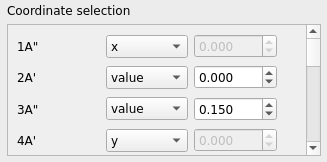
\includegraphics[width=0.8\textwidth]{img/coord_select.png}
        \caption{Example of a \texttt{CoordinateSelector} being used in a parameter container.}
        \label{fig:coord_select}
    \end{minipage}\hfill\begin{minipage}[t]{.47\textwidth}
        \centering
        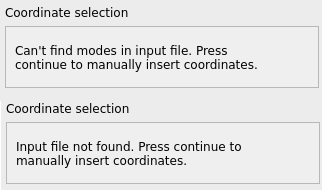
\includegraphics[width=0.8\textwidth]{img/coord_select_error.png}
        \caption{Special messages in \texttt{CoordinateSelector} that occur when mode labels cannot be found, or when the \texttt{input} file does not exist.}
        \label{fig:coord_select_error}
    \end{minipage}
\end{figure}

\subsubsection{Finding mode labels}\label{sssec:findmodelabels}

The first task is to implement a \texttt{findModeLabels} method that can obtain mode labels from the \texttt{input} file. Unfortunately, mode labels can be found in different sections, depending on the nature of the simulation. For MCTDH, mode labels are generally found in the \texttt{SPF-BASIS-SECTION} (or \texttt{SBASIS-SECTION} in older \texttt{input} files), and for DD-vMCG, mode labels are \textit{sometimes} found in the \texttt{nmode} subsection of a \texttt{INITIAL-GEOMETRY-SECTION} or the \texttt{DD-GB-SECTION}. Information in these sections can be obtained using regular expressions as the sections end with the phrase \texttt{END-} then the name of the section.

As an example, information in the \texttt{SPF-BASIS-} or \texttt{SBASIS-SECTION} is selected using \mintinline{python}{r'S(?:PF-)?BASIS-SECTION\s*\n(.*)\nend-s(?:pf-)?basis-section'} with the \texttt{re.DOTALL} flag. Mode labels here are written in the form \texttt{mode\_label1 , mode\_label2 , ... = nspf1 , nspf2 , ...} where \texttt{nspf} is a digit (or sometimes the special keyword \texttt{id}). Another regex is used to select characters before the equals sign, and have the characters split by a comma (using \mintinline{python}{.split(',')}) and whitespace removed (using \texttt{.strip()}) in a list comprehension. Note that other keywords may be defined here such as \texttt{packets} or \texttt{gwp-type} which we ignore as these are not mode labels. For the \texttt{nmode} subsection each mode label is the first sequence of characters on a new line. Explanations for all regexes are found in \S\ref{ssec:regex}.

While the implementation above can cover a wide range of cases, it is unfortunately not exhaustive. For example, for ML-MCTDH simulations, mode labels are given in an \texttt{ML-BASIS-SECTION} using a tree structure (Fig. \ref{fig:mcdth_trees}). For some DD-vMCG simulations no mode labels are given in the \texttt{input}, in which they are read from the database file. Special parameters such as \texttt{elcont} given in other sections change the name of certain mode labels (for this case \texttt{el} is changed to \texttt{Elcont}), and so on. These particular limitations are discussed further in \S\ref{sssec:input_parser}. If an \texttt{input} file exists but no mode labels can be found using the above implementation an empty list is returned from \texttt{findModeLabels} which can be detected and cause a special message to appear (Fig. \ref{fig:coord_select_error}).

\subsubsection{Adding subwidgets}

Assuming we have a list of mode labels however, we can now build the widget around this. We must manually create the widget using code instead of in Qt Designer as the number of mode labels is variable. In the method \texttt{addModeLabels}, a subwidget is created for each mode label that includes the \texttt{QLabel} for the label, the combo box to select \(x\), \(y\), or ``value'' from, and the spinbox to choose the value. If there is only one label, \(x\) is given as the only option in the combo box. Otherwise, by default the first two labels are chosen to be \(x\) and \(y\), and the rest are set to ``value'' using \mintinline{python}{select.setCurrentIndex(min(i, 2))} where \texttt{select} is the name of the combo box. For the first two labels, the spin box is also disabled accordingly.

We also need to connect signals to these subwidgets so they behave as expected. In particular, the spinbox should only be enabled if ``value'' is selected, and only one DOF can be chosen as \(x\) and \(y\). In the \texttt{addModeLabels} method, each combo box is connected to a slot named \texttt{selectChanged} for this purpose. When this slot is triggered, firstly, we need to know which subwidget the combo box that had been changed is in. This can be done with the aid of PyQt's \texttt{self.sender()} method, such that the index can be obtained using \mintinline{python}{self.layout().indexOf(self.sender().parent())}, which allows us to find the specific spinbox to enable or disable. Secondly, if the user picks \(x\) or \(y\), then any \(x\) or \(y\) in other subwidgets need to be changed to ``value''. We iterate through all the subwidgets in the coordinate selector and change the combo box to ``value'' if they match the index selected, using \mintinline{python}{self.layout().itemAt(i).widget()} to obtain the subwidget attribute. The subwidget index that \texttt{self.sender()} is in is skipped, of course.

We will also need to provide a \texttt{clearWidget} method. If the user changes directory with a different set of mode labels, the subwidgets in the coordinate selector need to be cleared before new ones are added, done by iterating through all subwidgets and using the \texttt{deleteLater} method. Then, a \texttt{refresh} method to combine clearing the widget and adding new subwidgets with \texttt{addModeLabels}.

\subsubsection{An aside: Splitting the \texttt{AnalysisTab} constructor}

In order to integrate this with an analysis method, the \texttt{optionSelected} in the analysis class can be overridden to refresh the coordinate selector when the radio option containing the widget is selected. This allows the widget to generate its subwidgets on-demand rather than during its intialisation. Because \texttt{optionSelected} is called when any of the analysis radio buttons are selected, in order to ensure that the options inside the selector do not reset when selecting another radio button and returning, the current mode labels are saved in an attribute \mintinline{python}{self.mode_labels}. If \texttt{findModeLabels} returns an identical list, \texttt{refresh} does not need to do anything.

However, we also want to refresh the widget when the user changes the directory. This can be done by connecting the \texttt{textChanged} signal in of the text edit in the directory widget to the \texttt{optionSelected} slot also. Alternatively, it can be connected to \texttt{refresh} directly, but it is better to be general if other custom widgets similar to coordinate selector are implemented in the future. However, since accessing the directory widget requires the pointer to the main window, which is given via \texttt{.window()}, there is a problem when we add the connection in the analysis class constructor. The \texttt{.window()} method does not work in \texttt{\_\_init\_\_}, instead returning a pointer to itself, which means that any attempted connections made in the constructor do not work (as the analysis tab does not contain a directory widget itself). This is also a problem when implementations of \texttt{runCmd} and \texttt{checkFileExists} depend on menu options in the main window (\S\ref{ssec:additional_options}).

The reason why \texttt{.window()} does not work in \texttt{\_\_init\_\_} is because \texttt{.window()} recursively finds the parent object of the widget until it reaches the top level widget (main window). When a widget such as \texttt{CoordinateSelector} is initialised, the children and parents of the widget are not set until the end of \texttt{\_\_init\_\_}. Solving this issue requires splitting the constructor for the \texttt{AnalysisTab} class in two. We can delay creating connections until the final constructor is called, which is in the \texttt{AnalysisMain} class. We create a method named \texttt{activate} containing everything previously in the constructor except loading the .ui file, meaning that connections and dictionaries mentioned in \S\ref{ssec:analysistab} are given in \texttt{activate} instead. Then, in the constructor of the \texttt{AnalysisMain} class, \texttt{activate} is called for all the analysis classes to provide full functionality.

\subsubsection{Using coordinate selector in analysis methods}

The premise of the \texttt{CoordinateSelector} widget is to provide the parameters required in the ``Change coordinate selection'' submenu of the \texttt{showsys} command line program. On each line in this menu, the user types the mode label, followed by \texttt{x}, \texttt{y} or a constant number. We can create a method \texttt{\_\_str\_\_} to convert the user's choices in the GUI to the text that the user would type in the coordinate selection submenu. This can then be used in the analysis method as part of the \texttt{input} parameter to \texttt{runCmd}. Implementing \texttt{\_\_str\_\_} involves simply iterating through all subwidgets, then adding its mode label and either \texttt{x} or \texttt{y} from the combo box or the value from the spinbox, before attaching a new line at the end. Note that an error occurs when no DOF is selected as \(x\) in the CLI: this is replicated in the \texttt{\_\_str\_\_} method also. If \texttt{findModeLabels} did not return any mode labels, then \texttt{\_\_str\_\_} will return an empty string. This can be identified in the analysis program and have an alternative implementation as necessary.

In addition, a similar implementation can be used to obtain the mode label for chosen as \(x\) or \(y\). This is particularly useful as we can use this to include the mode label as axis labels during plotting.

\subsection{Contour plots}\label{ssec:contour}

In the previous section, we developed a widget that allows the user to select the values for coordinate to use for the \(x\) and \(y\) axes. Using \texttt{showsys}, this will produce a 3D contour plot with the contours representing the values on the \(z\) axis. Unfortunately, as mentioned in \S\ref{ssec:plot_widget}, pyqtgraph does not have a built-in method to produce a contour plot as of the time of writing this dissertation. It does however contain a method to produce an \textit{isocurve}, which is a single contour line, which we can use to add a \texttt{plotContours} method in our \texttt{CustomPlotWidget}.

The pyqtgraph \texttt{IsocurveItem} has two main parameters. The first is a matrix which contain the values of \(z\) for each coordinate in \(x\) and \(y\). The second is the level of the isocurve, which corresponds the value of \(z\) that the isocurve is drawn on. The contour plot can then be implemented using a for loop over a range of levels. However, note that the \texttt{IsocurveItem} does not have \texttt{x} or \texttt{y} as parameters. Instead, the bounds of the data array \texttt{z} are implicitly assumed to be the indices of the array (e.g.~passing a \(30\times 30\) array plots it over (1, 1)--(30, 30)). To fix this, we can use PyQt's \texttt{QtGui.QTransform} class to define a translation and scale to apply to the isocurve, assuming that the values in \texttt{x} and \texttt{y} are linearly spaced (Listing \ref{lst:isocurve_transform}).

\begin{code}\begin{minted}{python}
tr = QtGui.QTransform()
tr.translate(x.min(), y.min())
tr.scale((x.max() - x.min()) / np.shape(z)[0], (y.max() - y.min()) / np.shape(z)[1])
for i in range(len(levels)):
    c = pg.IsocurveItem(data=z, level=levels[i], pen=colours[i])
    c.setTransform(tr)
    self.getPlotItem().addItem(c) # add to plot widget
\end{minted}
\caption{Code snippet for transforming the isocurve to align with the arrays \texttt{x} and \texttt{y}. \texttt{levels} and \texttt{colours} are the list of levels and line colours for each isocurve.}
\label{lst:isocurve_transform}
\end{code}

We can then create a method \texttt{plotContours} based on listing \ref{lst:isocurve_transform} that has \texttt{x}, \texttt{y} arrays, and the matrix \texttt{z} as parameters where the length of \texttt{x} and \texttt{y} match the shape of \texttt{z}. Then we can add an additional parameter \texttt{levels} which can be sepcified either with a list of \(z\)-values to draw isocurves over, or an integer for the size of list which is generated from equally spaced values between \texttt{z.min()} and \texttt{z.max()}.

Lastly, it would also be useful to include a colourbar, such that an isocurve having a particular colour on the colourbar represents that value of \(z\). There is a convenience function in pyqtgraph that allows this using \mintinline{python}{self.getPlotItem().addColorBar}, but is meant to be coupled with an image plot, which is a required parameter. We do not actually want to include an image plot over the contours, so we can simply pass an empty image map \texttt{pyqtgraph.ImageItem()} into the parameter. This colourbar can be hidden at startup and in \texttt{AnalysisTab.reset} and is only shown when visualising a contour plot using the \texttt{plotContours} method.

The colourbar also requires a colour map, which defines the colour for each value in the colour bar. One can use the \texttt{pyqtgraph.colormap.get} to select from a default collection included with pyqtgraph---for this GUI, the ``CET-R4'' colour map was used. Then, in the implementation for \texttt{plotContours}, a list of colours can be obtained from the list of levels using \mintinline{python}{self.colourmap.getLookupTable} with parameters \mintinline{python}{nPts=len(levels), mode=pyqtgraph.ColorMap.QCOLOR}. To ensure the numerical tick labels are correct, the colour bar's \texttt{setLevels} method can be used with \texttt{z.min()} and \texttt{z.max()} as parameters.

\subsubsection{\texttt{showpes}}\label{sssec:showpes}

\begin{wrapfigure}{r}{0.45\textwidth}
    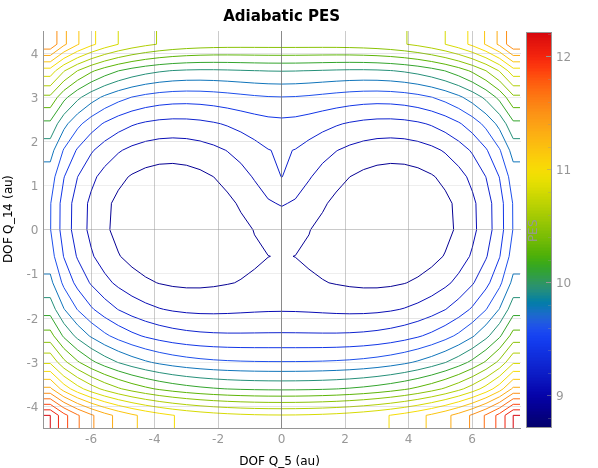
\includegraphics[width=\linewidth]{img/but_pes_gui.png} 
    \caption{Contour plot of the PES of the lower excited state of butatriene, as shown in the GUI. Compare Fig. \ref{fig:conical_intersection}.}
    \label{fig:but_pes_gui}
    \end{wrapfigure}

One of the tasks that \texttt{showsys} can perform is to plot the PES of the system. If we would like to only plot the PES, the flag \texttt{-pes} can be added as a parameter; this will save time that is otherwise spent reading the \texttt{psi} file. Normally when using the CLI, the user would directly call \textit{gnuplot} using the ``plot to screen'' option (Option 1, listing \ref{lst:showsys_menu}). To obtain data in a file, the ``save data to an xyz file'' option can be used (Option 5).

The \texttt{showpes} method, which calls the \texttt{showsys} program to obtain the PES, has parameters to show the either the diabatic and adiabatic PES, the state to select, and the coordinates provided by the coordinate selector (\S\ref{ssec:coordinate_selection}). These correspond to option 10, ``change plot task'', option 60, ``change state selection'', and option 20 respectively. As mentioned before, these parameters are no longer given to the call to the command line but using the \texttt{input} parameter, which must a string containing the keystrokes required as if the Python code was simulating a user selecting these options on a CLI. For example, to select the task of plotting the diabatic PES, one types 10, enter, 2 to select the correct option ``plot diabatic pes'', enter. So the input string is \mintinline{python}{'10\n2\n'}. A similar implementation is used to select the state.

The keystrokes required to select the coordinates can be produced with the aid of \texttt{CoordinateSelector.\_\_str\_\_}, such that the input string is simply \mintinline{python}{f'20\n{str(self.showpes_coord)}\n'}, where \mintinline{python}{self.showpes_coord} is the coordinate selector instance in the \texttt{showpes} parameter container. However, in case the coordinate selector did not manage to obtain the mode labels, \texttt{QtWidgets.QInputDialog.getMultiLineText} is used to obtain the input, where the experience is identical to writing down the coordinates manually in the CLI except the intermediate output containing the list of mode labels to choose from is not included.

Finally, the ``save data to an xyz file'' option is selected using 5, enter, and the query for the saved filename of the output is entered as \texttt{pes.xyz}. 0 must then be typed to exit the program, otherwise an error occurs as the program is terminated while still waiting for user input. The inputs for interacting with each submenu are concatenated before the command is run. This produces the output PES file which can be read. \texttt{showsys} also writes a .log file of details; since the standard output is not very illuminating (just lists and lists of options), the text in the text widget is replaced with the contents of the log file.

If the user did not select a \(y\) value, columns for a 1D line plot are output, which can be parsed and plotted as normal per listing \ref{lst:generic_analysis}. Otherwise, the PES file contains columns for \(x\), \(y\), and \(z\). \(x\) coordinates are incremented for each \(y\) value, then \(y\) values are incremented, producing a \(z\) value at each coordinate grid. The column format for \(z\) is unfortunately not the format that is required for \texttt{plotContours}, which require a grid of \(z\) values. As such, a conversion is necessary, where the 1D \(z\) column is reshaped into a 2D matrix with the size of the \(x\) and \(y\) arrays (listing \ref{lst:xyz2grid}).

\begin{code}\begin{minted}{python}
x = np.unique(self.window().data[:, 0])
y = np.unique(self.window().data[:, 1])
z = np.array(self.window().data[:, 2]).reshape(y.shape[0], x.shape[0]).T
\end{minted}
\caption{Conversion from the data in a .xyz file to \texttt{x} and \texttt{y} arrays and a \texttt{z} matrix.}
\label{lst:xyz2grid}
\end{code}

These values can then be used as parameters for \texttt{plotContours}. The \texttt{xcoord} and \texttt{ycoord} attributes of the coordinate selector can be used in the labels for the resulting plot. An example can be seen in Fig. \ref{fig:but_pes_gui}.

\subsubsection{\texttt{showd2d}}\label{sssec:showd2d}

Another task that \texttt{showsys} can perform is to plot the 2D reduced density evolution, i.e.~the 2D equivalent of \texttt{showd1d} (\S\ref{sssec:showd1d}). There is also a non-menu based program that performs the same task known as \texttt{dengen}, but was not interfaced with as \texttt{dengen} does not produce the correct output, either crashing due to a segmentation fault or producing an output file with only \texttt{NaN}s.

The parameter \texttt{-nopes} can be passed to save time reading the \texttt{oper} file. The \texttt{showd2d} analysis method output will be an animated contour plot, combining implementations for animated plots (\S\ref{ssec:animated_plots}) and contour plots (\S\ref{ssec:contour}). The underlying data plot will have \(x\), \(y\), \(z\), and \(t\) values, making it essentially a 4D array. Here, no parameter is needed to select adiabatic or diabatic regimes; the parameters are for the state and coordinate selection only. Otherwise, the creation of the input string is identical to \S\ref{sssec:showpes}. The case where a \(y\) coordinate is not selected does not have to be handled as an information popup can be created telling the user to use \texttt{showd1d} instead.

The difficult part of implementing this method is due to the format of the output .xyz file, as there is no column for time as there was in \texttt{showd1d}. Instead, the format is identical to the previous section with columns for \(x\), \(y\), and \(z\), but with two empty lines between each time interval, before the \(x\), \(y\), and \(z\) columns for the next time interval is included. These two empty lines can be matched using the regular expression \mintinline{python}{r'(?:\n\s*){3}'}. The \texttt{\textbackslash{}s*} is required as one of the blank lines contain whitespace so matching three consecutive new lines does not work.

Therefore, to create the data array for this analysis the entire output file must be read, then split into individual xyz blocks using the \texttt{re.split} function with the regex provided above. Each of the resulting blocks can then be converted into a grid format using listing \ref{lst:xyz2grid} and added to a list; however, the \texttt{x} and \texttt{y} arrays only need to be created using the data from the first time interval, as we assume that \texttt{x} and \texttt{y} are the same for all time intervals. The resulting list of NumPy arrays is then converted into one big 3D NumPy array that represents the time evolution of the \(z\)-grid.

Afterwards, the media scrubber's \texttt{valueChanged} is disconnected and reconnected as per the implementation in \texttt{showd1d}. For the slot's implementation, the use of \mintinline{python}{self.window().plot.listDataItems()} does not work as this only retrieves \texttt{PlotDataItem}s, not \texttt{IsocurveItem}s. These can instead be retrieved using \mintinline{python}{self.window().plot.getPlotItem().items}, which is a list of all objects in the plot, which for a contour plot only consists of \texttt{IsocurveItem}s. The data for each isocurve is then updated using \texttt{.setData} with the corresponding \(z\) data for the time interval representing the scrubber's position.

Finally, when plotting the contour plot for the first time interval, the \texttt{levels} parameter should be a list containing the minimum and maximum levels of \(z\) over all time intervals to get a better representation of the true range of values, as otherwise only contour levels between the minimum and maximum of the first time interval are shown.

\subsection{New analysis functions}\label{ssec:new_analysis}

As mentioned in \S\ref{ssec:aims}, the analysis GUI also contains a handful of analysis options not previously implemented in Fortran. These new analyses are all in the topic of DD-vMCG (\S\ref{ssec:ddvmcg}), which is comparatively a much newer addition to the \textit{Quantics} package, and are written purely in Python.

At the moment, these analyses are simply methods in an analysis class that are called from the selection of the relevant radio button (\S\ref{ssec:analysistab}). Should future work on these Python analyses make the file size too large, individual analyses could potentially be moved to a new file and parameters added to them. These files can simply be imported and the method in the analysis class call them with parameters selected by the user in the GUI.

\subsubsection{\texttt{calcrate}}\label{sssec:calcrate}

In a DD-vMCG calculation, any calls to external quantum chemistry programs such as \textit{Gaussian} or \textit{Molpro} (\S\ref{ssec:ddvmcg}) are recorded in the \texttt{log} file. The \texttt{calcrate} method reads this file and plots how many calls are made at each time interval. The part of the \texttt{log} file we are interested in is in the form of listing \ref{lst:log_qc}.
\begin{code}\begin{minted}{text}
 time[fs]       24.000
DD Update requires new point at:    24.229195
No. QC calculations :     1
Generating DB Point for GWP :     1
 Generating symmetry replica :     2
Propagating diabatic states to DB record:          3251   from: 3213
Propagating diabatic states to DB record:          3252   from: 3214
DD Update requires new point at:    24.229195
No. QC calculations :     1
Generating DB Point for GWP :    25
 Generating symmetry replica :     2
Propagating diabatic states to DB record:          3253   from: 787
Propagating diabatic states to DB record:          3254   from: 788
DD Update requires new point at:    24.316975
\end{minted}
\caption{A text snippet of recorded calls to QC programs in a \texttt{log} file.}
\label{lst:log_qc}
\end{code}
The algorithm is as follows. The file is read, and for each line, if it contains the sequence ``\texttt{time[fs]}'', the time is appended to the list \texttt{times} using the regex \mintinline{python}{r'[+-]?\d+(?:\.\d*)?'} (This is a part of the float regex, explained in \S\ref{ssec:regex}). Then, a new entry is appended to the list \texttt{n\_calcs} initialised to 0. If it contains the sequence ``\texttt{No. QC calculations}'', the following number is added to the last entry of the \texttt{n\_calcs} list. \texttt{n\_calcs} can then be plotted against \texttt{times}. The contents of the \texttt{log} file are also written to the text widget, for good measure.

\subsubsection{\texttt{querydb}}\label{sssec:querydb}

As the QC database is implemented using SQLite, it can be queried using SQL. The \texttt{querydb} allows the user to use any SQL query to inspect the QC database and have the results returned in a formatted table in the text widget. To connect to the QC database one can use the \texttt{sqlite3} package, part of the Python standard library, and to execute a query one can use code in the form of listing \ref{lst:connect_db}.
\begin{code}\begin{minted}{python}
con = sqlite3.connect('file:/home/user/sim/dd_data/database.sql?mode=ro', uri=True)
cur = con.cursor()
res = cur.execute(query).fetchall() # can repeat for multiple queries
con.close()
\end{minted}
\caption{Code snippet for connecting to an SQLite database and executing an SQL query named \texttt{query}.}
\label{lst:connect_db}
\end{code}

The QC database is always called \texttt{database.sql}. The mode \texttt{ro} opens the database in read-only mode, such that any write queries generate an exception. A checkbox is given to the user to indicate whether they want to disable read only mode---if this is checked, the database is opened using mode \texttt{rw} (read-write). The user is then given a \texttt{QPlainTextEdit}, which can recieve multiline strings (this is the same class the text widget inherits from, except with editing enabled), to input an SQL query, which is executed using listing \ref{lst:connect_db}. For long SQL queries, the height of the \texttt{QPlainTextEdit} automatically adjusts itself such that all of the query is visible using the \texttt{sqlChanged} slot.

The returned result from the query is a table in the form of a list of tuples, where each tuple represents a row. To display this we can use the text widget, but simply using \mintinline{python}{str} to convert this table into a string is not very helpful as it is not nicely formatted---each cell in the table may have a variable size so columns are not necessarily aligned. To fix this we can create a method in \texttt{CustomTextWidget} named \texttt{writeTable}.

This method uses the Python \texttt{format} method to pad cells to a fixed size. For example, \mintinline{python}|'{:>15}'.format(string)| pads a string to 15 characters aligned to the right, and \mintinline{python}|'{: .8e}'.format(num)| formats a float to always use scientific notation using 8 decimal places, and prepend a space for positive numbers (as negative numbers require an additional character). It also has other parameters such as \texttt{colwidth} to vary the cell size, whose implementation requires formatting the formatter which can be done using an \(f\)-string. At the moment, the \texttt{CustomTextWidget.writeTable} method is used only for \texttt{querydb}, but in the future, new analyses using Python may find it useful.

\subsubsection{\texttt{ddpesgeo}}\label{sssec:ddpesgeo}

The final analysis program, unconvincingly named \texttt{ddpesgeo}, is dedicated to finding the geometries of the molecular that correspond to certain energies in the PES of a QC database. This can be used by the user to find particular molecular geometries corresponding to minima or conical intersections in the PES (discussed in \S\ref{ssec:ddvmcg}). The user can choose between the diabatic and adiabatic potential energy surfaces using a combo box, and can select geometries between two energies, in which a search is performed over all states, or geometries where the energies between two states coincide within a specified tolerance, in which the user specifies the first state and a search is performed over the second state\footnote{Matches over more than two states are not implemented as this is very uncommon and performing the search is more computationally costly.}. This choice is given via two radio boxes. As the parameters are different for each option, the radio box is connected to a signal which shows/hides two parameter subcontainers with a similar implementation to \S\ref{ssec:per_analysis}.

The specific implementation is dependent on the version of the QC database. The tables present and column names for each table are different for each version, of which the latest version is version 4. This value is found in the \texttt{dbversion} column of the \texttt{versions} table. At the moment, \texttt{ddpesgeo} is only configured to work with version 4: for other versions an error is returned to the user.

The energies for state \texttt{s} are located in the \texttt{eng\_\{s\}} column for the \texttt{apes} table and \texttt{eng\_\{s\}\_\{s\}} column for the \texttt{pes} table (nonidentical numbers refer to couplings). A dictionary named \texttt{state\_name} is created mapping state number to column name for convenience. To perform a search over all states the number of states must be known; this value is found in the \texttt{nroot} column of the \texttt{refdb} table. Then, for each state, a query is made to the database. The values for the energy are located in a different table than the geometries, so the \texttt{pes} or \texttt{apes} and \texttt{geo} tables must be combined with a \textit{join}; since both tables contain the column \texttt{id} (which the join is performed over), tables can be merged together (temporarily) if two records share the same \texttt{id}.

For the energy between intervals task, the query is \mintinline{sql}{SELECT * FROM @table LEFT JOIN geo} \mintinline{sql}{USING(id) WHERE @state_name[s] BETWEEN @emin AND @emax;} where the \texttt{@} indicate variables inputted in Python using \(f\)-strings and the \texttt{*} selects all columns. For the matching energies task, the query is \mintinline{sql}{SELECT * FROM} \mintinline{sql}{@table LEFT JOIN geo USING(id) WHERE ABS(@state_name[s2] - @state_name[s1]) <= @tol;}.

\begin{wrapfigure}{l}{0.45\textwidth}
    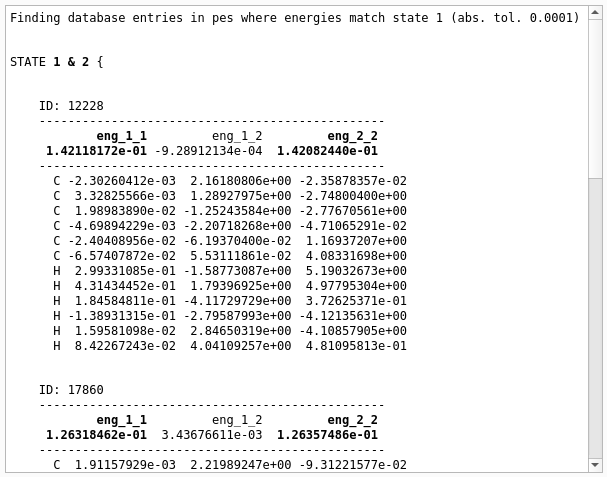
\includegraphics[width=\linewidth]{img/ddpesgeo.png} 
    \caption{Example output of a \texttt{ddpesgeo} analysis with the matching energies task.}
    \label{fig:ddpesgeo}
    \end{wrapfigure}

The results can then be written to the text widget inline inside the for loop, but to split responsibilities of querying the database and formatting the results, an intermediate dictionary \texttt{pesgeo} is created to store the results of each query. The dictionary has the state or states representing the key using a \mintinline{python}{frozenset} (an immutable set; here it only contains one or two items) and a list of entries where each entry is also a dictionary containing the ID, energies, and a NumPy array of the geometries, whose conversion is made simple using the \texttt{geo} table column names, which are \texttt{x\_\{n\}}, \texttt{y\_\{n\}}, and \texttt{z\_\{n\}} for each atom \texttt{n}.

The \texttt{pesgeo} dictionary is then formatted per Fig. \ref{fig:ddpesgeo}. The particular format of the geometries shown is in a format that can be read by a program such as \textit{Jmol}\footnote{\url{https://jmol.sourceforge.net/}} which can view the structure of the molecule. Firstly, the selected entries are grouped by their state, or pairs of state if the task is to find matching energies, using two curly braces \texttt{\{...\}}. This allows the user to select any one particular state or pairs of states more easily. Secondly, the ID and energies of the matching entry are printed. The column names of the \texttt{pes} or \texttt{apes} table can be retrieved using SQLite's special function \texttt{pragma\_table\_info}, from which the names can be selected using \mintinline{sql}{SELECT name FROM pragma_table_info("@table");}. Thirdly, the geometries can be formatted nicely using the NumPy method \texttt{np.array2string}, passing a formatter such as the ones mentioned in \S\ref{sssec:querydb}. Lastly, we can highlight the matching energies if we use \texttt{QPlainTextEdit}'s \texttt{appendHtml} method instead of \texttt{setText} to obtain HTML formatting capabilities, namely allowing bold text via the \mintinline{html}{<b></b>} tag. This does mean normal line breaks do not work anymore. For some reason, breaking a line with \mintinline{html}{<br/>} does not work: instead, each line must be wrapped in a \mintinline{html}{<pre></pre>} tag before \mintinline{html}{<br/>} can be used.

\subsection{Additional options}\label{ssec:additional_options}

There are a number of additional options that can be selected in the ``Options'' menu, located in the menubar, that modify the behaviour of the GUI, intended to give more advanced users more control over certain aspects of the program. The first option is a \textit{timeout} option, which controls the time to wait for a command line program to return an output before giving up (killing the process), as well as the maximum time a SQL query can take. This value has no influence on how much time is allowed for the Python GUI to read files or plot the output, however.

Using a \texttt{QWidgetAction} to embed a \texttt{QDoubleSpinBox} in the menu (like in \S\ref{ssec:customising}), the user can select the timeout limit and the value can be accessed via \texttt{self.window().timeout.value()}, which can be input into the \texttt{timeout} parameter in \texttt{subprocess.run} and in \texttt{sqlite3.connect}.

As calls to most Fortran analysis programs leave behind a file, performing many analyses in the same directory will clutter the directory with many output files. These files are left behind after an analysis as generally, a file should not be deleted without the user's permission. Instead, the user is given the ``cleanup directory'' option, which allows them to delete all possible analysis output files in one click. To implement this, a list of patterns to match is given in a \textit{glob}-type format, where, for example, the glob pattern \texttt{qdq\_*.pl} matches all possible \texttt{qdq} output files for any DOF and state (\S\ref{sssec:qdq}). For each pattern \texttt{glob}, a list of analysis output files that exist in the directory \texttt{files} can be produced using \mintinline{python}{files.extend(list(self.dir.cwd.glob(glob)))}.

The names of each file found is then given in a confirmation question using \texttt{QtWidgets.QMessageBox.question} (Fig. \ref{fig:cleanup}). If the user selects ``Yes'', each file will be deleted using \texttt{file.unlink()}, and a confirmation popup is given. Otherwise, the operation is cancelled. If \texttt{files} is empty, a popup indicating no files were found is shown.

\begin{figure}[h]
    \centering
    \begin{minipage}[t]{.47\textwidth}
        \centering
        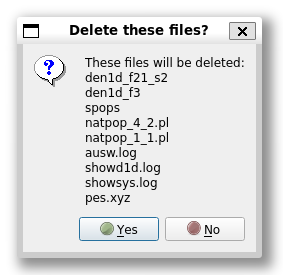
\includegraphics[width=0.6\textwidth]{img/cleanup.png}
        \caption{Example of the confirmation popup that appears when cleaning up output files.}
        \label{fig:cleanup}
    \end{minipage}\hfill\begin{minipage}[t]{.47\textwidth}
        \centering
        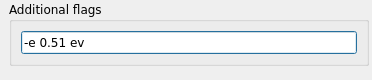
\includegraphics[width=0.8\textwidth]{img/add_flags.png}
        \caption{An additional \texttt{QGroupBox} that appears when the ``Allow additional flags'' option is selected. Here, the flag \texttt{-e} tells \texttt{autospec} to shift the energies by this amount.}
        \label{fig:add_flags}
    \end{minipage}
\end{figure}

As previously discussed in \S\ref{ssec:per_analysis}, some analysis programs have many optional parameters, some of which are only used in niche cases. As such, these options are not included in the parameter containers, but the advanced user is still free to specify them by including them in the ``Additional flags box''. This box is normally hidden, but can be enabled via the options menu. On any call to the \texttt{runCmd} method, flags input into the additional flags box are split into individual parameters using \texttt{shlex.split}, then inserted into the arguments list. The flags must be inserted before the positional parameters since it appears that Fortran stops reading any further arguments if all the positional parameters are received. This can be done using \mintinline{python}{args[1:1] = add_flags}.

One of the parameters the user can input into the additional flags box can change the required files that an analysis method needs, namely, for analysis programs that read the \texttt{psi} file, the flag \texttt{-r} or \texttt{-rst} reads the \texttt{restart} file instead, which contains the information (including contents of \texttt{psi}) to continue a simulation if it had been stopped abruptly, or the user wants to extend the propagation time. As such, the implementation that disables the ``Analyse'' button must be disabled if the user.

The final option given is the option to disable any calls to the Fortran analysis programs completely, named ``No command mode''. The reason why someone may do this is if they have the analysis output from the command line program already, and they only want the GUI to plot this output, without needing to call the program again. This is particularly useful if the analysis takes a long time (e.g.~2D contour plots of the PES in a DD-vMCG simulation). In this case, a manual call on the CLI can be made, and run in the background without needing the GUI to be open all the time, or the analysis can be performed on an HPC cluster and only the output file needs to be transmitted back to the user. When this mode is turned on, the file-checking implementation is disabled, but the user should still ensure the parameters are set such that the correct file is read, otherwise an error will occur.

\section{Documentation and testing}\label{sec:doc_test}

\subsection{User guide}\label{ssec:user_guide}

\begin{figure}[h]
    \centering
    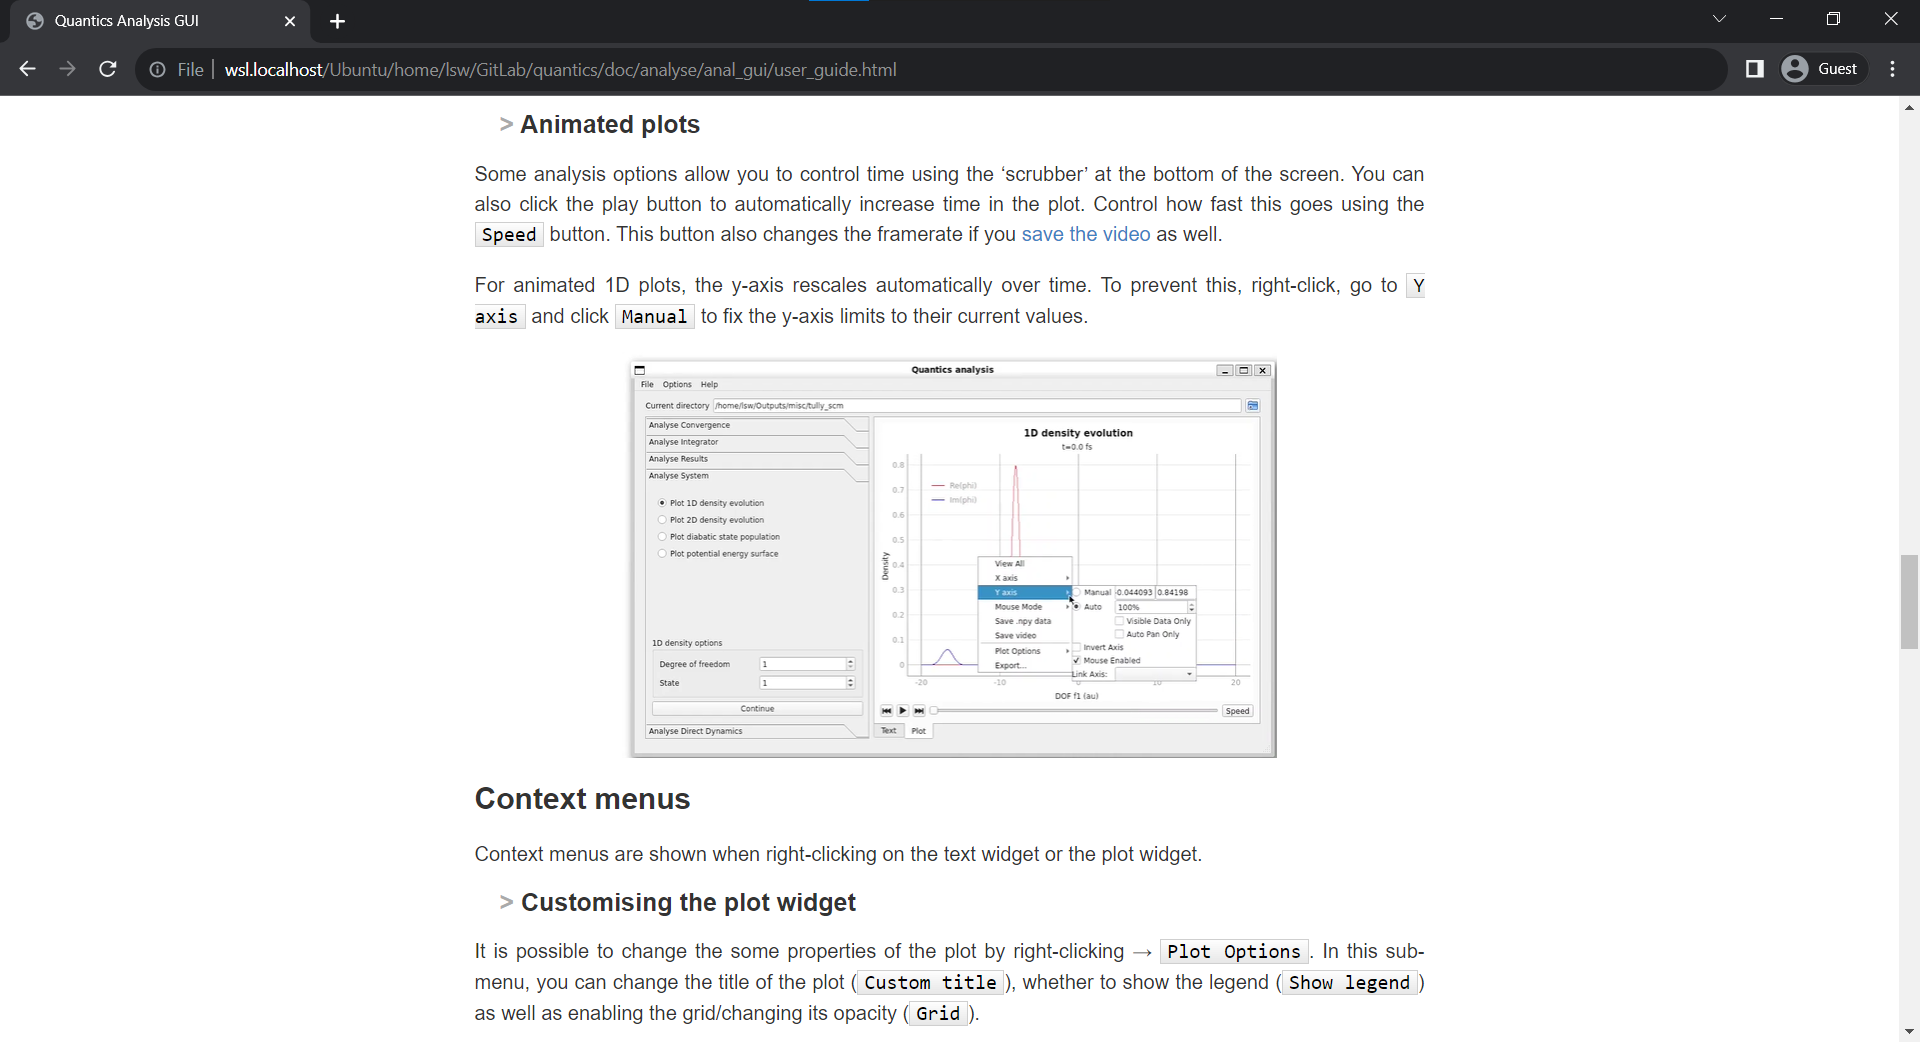
\includegraphics[width=0.9\textwidth]{img/doc.png}
    \caption{Sample of the user documentation as shown in \textit{Google Chrome}. In the centre a short video tutorial is shown.}
    \label{fig:doc}
\end{figure}

\noindent The Python package has a \texttt{README.md} file (see listing \ref{lst:dir_files}) with details on the basic installation and opening of the GUI. However, for describing the usage inside the GUI, a user guide is created. For maximum usability, the user should not have to look up any documentation, but there should still be help provided if the user needs it. This user guide contain tutorials on how to perform certain tasks in the GUI, such as navigation in the plot widget, selecting coordinates using the coodinate selector (\S\ref{ssec:coordinate_selection}), as well as a brief explanation of some more advanced options (\S\ref{ssec:additional_options}). The location of the user guide is in the \texttt{doc/} directory in the \textit{Quantics} repository. There is an HTML file which can be opened in a web browser, with an accompanying stylesheet (CSS file) and a folder for media in the guide. A link to the user documentation is also present in the ``Help'' menu in the menubar of the GUI.

The stylesheet describes how the HTML elements (such as paragraphs, hyperlinks, titles) are presented to the user. The design is purposefully minimalistic, using a sans-serif font to ease reading on a computer screen, and setting a maximum body width so that the user does not need to move their head to see text at the edge of their screen. The CSS file also contains a presentation for GUI buttons using the HTML \mintinline{html}{<span class="button"></span>}, useful for indicating which part of the text represent items on the GUI.

There are a number of short video tutorials embedded into the web document. These videos are generally less than 20 seconds long and provide the exact instructions for performing a task, which may be more useful for visual learners. These videos were recorded using OBS, a screen recorder. To keep the file size of the videos low, the bitrate of the video was set lower than the default value (1700 Kbps), the framerate set to 30 FPS, and the captured video was sped up by 33\% using the \textit{FFmpeg} command \texttt{ffmpeg -i video.mp4 -filter:v 'setpts=0.75*PTS' -an out.mp4} (framerate is unchanged by this command). The \texttt{-an} flag removes the audio track from the video, since an audio track is still saved even if all input devices are muted in OBS.

To embed these videos in an HTML document the \mintinline{html}{<video>} tag is used. To allow autoplay of the video, which prevents the user needing to interact with the webpage, the following attributes need to be included inside the tag: \texttt{autoplay}, \texttt{muted} (as most browsers refuse to autoplay videos with sound), \texttt{loop} (to make the video repeat itself), and \texttt{playsinline} (some mobile web browsers need this since videos can ``pop out'' on mobile devices).

A file containing developer documentation was also set out as a task. Due to time limitations, it was never produced. The codebase already contains plenty of comments and docstrings that help future developers to understand the code, so the intended goal of this documentation was on how to edit the .ui files using Qt Designer (e.g.~adding widgets to parameter containers), and design principles inside the analysis classes (e.g.~what circumstances would it be suitable to override \texttt{activate} or \texttt{optionSelected}).

\subsection{Unit testing}\label{ssec:unit_testing}

Software testing is an important aspect in most programs to ensure that the behaviour of the program aligns with the user's expectations, and to identify the situations where this is not the case. At the lowest level, this is called \textit{unit testing} where the individual methods or functions are analysed to ensure that for a given input, the output of the method or function is correct.\textsuperscript{\cite{testing}}

Due to the nature of the project, testing is usually performed manually. This is because it is generally easier to navigate the GUI on the screen than by code, and that the output of most analyses are visual (in a plot), in which a human is generally required to check that the graphics look correct. However, there are some methods that can be tested automatically using code. In particular, the methods that are focused on for testing are methods that do not rely on external programs, as we only want to check the code written for this project\footnote{It is still possible to test these methods using a \textit{mock} to replace the interface to the external program. This is called \textit{mock testing}, but is out of scope for this project.}, and methods whose purpose is not to solely produce a visualisation. These exclude any method that calls a Fortran program, or consist mostly of calls to an external package such as \texttt{sqlite3}.

The methods that satisfy these conditions are \texttt{readFloats} (\S\ref{sssec:read_floats}), \texttt{rdtiming} (the sort functionality; \S\ref{sssec:rdtiming}), \texttt{calcrate} (\S\ref{sssec:calcrate}), \texttt{ddpesgeo} (\S\ref{sssec:ddpesgeo}), \texttt{writeTable} (part of \S\ref{sssec:querydb}), and \texttt{findModeLabels} (\S\ref{sssec:findmodelabels}). However, the incomplete nature of \texttt{findModeLabels} means that its implementation is not at a stage where it is particularly suitable to be tested. With the exception of \texttt{ddpesgeo}, whose unit test was not implemented due to time limitations, the aforementioned methods are tested in the \texttt{tests/} subdirectory of the \texttt{analysis\_gui} package.

In order to perform unit tests the \texttt{unittest} module is used from the Python standard library. It provides a \texttt{TestCase} class which can be inherited from to obtain methods such as \texttt{assertEqual}, \texttt{assertTrue}, etc. to check the values of a certain variable is as expected. However, to begin unit testing we must open the GUI inside of a test, without making it visible. To do this we use the \texttt{TestCase} class' \texttt{setUp} and \texttt{tearDown} methods, which can be overridden to perform an action before each test (open the GUI), and after each test respectively (close the GUI). This is implemented in listing \ref{lst:test_class}

\begin{code}\begin{minted}{python}
class TestClass(unittest.TestCase):
    def setUp(self):
        self.app = main_window.QtWidgets.QApplication(sys.argv)
        self.window = main_window.AnalysisMain()
    # test methods go here ...
    def tearDown(self):
        self.window.close()
        self.app.quit()
        del self.app # required to prevent errors with auto garbage collection
\end{minted}
\caption{Opening a GUI inside a class such that it can be tested.}
\label{lst:test_class}
\end{code}

Tests for the analysis methods are stored in a file named \texttt{test\_analyses.py} and the rest (\texttt{readFloats} and \texttt{writeTable}) are stored in a file named \texttt{test\_misc.py}. Normally, the tests are executed using \texttt{unittest.main()} in the Python file's main method, but as the files are stored in a package, executing Python files directly doesn't work (\S\ref{ssec:packaging}). Instead, we can use a \texttt{unittest.TestLoader()} to execute tests outside of the package directory, using the \texttt{top\_level\_dir} parameter (listing \ref{lst:run_tests}). This will also run all files in the directory starting with \texttt{test\_}, without needing to execute each file in the folder. A function which performs this is located in the \texttt{run\_tests.py} file. Alternatively, one can pass the \texttt{-test} flag to the \texttt{quantics\_analysis\_gui.py} file that is located outside of the package that calls this function.

\begin{code}\begin{minted}{python}
def runTests():
    loader = unittest.TestLoader()
    tests = loader.discover('analysis_gui.tests', pattern='test_*.py',
                            top_level_dir=Path(__file__).parents[2])
    testRunner = unittest.runner.TextTestRunner(verbosity=2)
    testRunner.run(tests)
\end{minted}
\caption{Code snippet of running test files in the \texttt{analysis\_gui/tests} folder. This function can be called directly within the package.}
\label{lst:run_tests}
\end{code}

Tests within each class are implemented using a method whose name starting with \texttt{test}, such as \texttt{testReadFloats}. For this method, a NumPy array is generated with random numbers, where the number of rows and number of columns are class constants and can be set by the developer. To ensure the function can read numbers in normal decimal format and scientific format, the mantissa and exponent are generated seperately, which provide a range of normal and very small/large numbers that can only be expressed in scientific notation. This array is then saved to a file, which \texttt{readFloat} reads. The test then asserts that the returned array is the same as the generated array. In addition, the performance can be tested using \texttt{time.perf\_counter()}; a test of reading a \(20000\times 5\) grid took 0.09 s on my machine, which is approximately the same rate as mentioned in \S\ref{sssec:read_floats}.

The NumPy array generated can also be used to test \texttt{writeTables}. Since this test succeeds the \texttt{readFloats} test, we know that \texttt{readFloats} works. If input the NumPy array into the text widget via \texttt{writeTables}, then \texttt{readFloats} should also be able to parse this as well. However, as \texttt{writeTables} only writes to a limited precision, \texttt{numpy.all\_close} is used instead of \texttt{numpy.array\_equal}.

In order to test the analysis functions we must have some example files for the analysis methods to read. These are called \textit{test fixtures}, and are located in the \texttt{fixtures/} subdirectory, which at the moment only contains a \texttt{timing} and \texttt{log} file for the two analyses we are about to test. We must then navigate to this directory and set all parameters directly using PyQt's slot methods such as \texttt{dir.edit.setText} and \texttt{analint.analyse.click()}.

To test that the \texttt{rdtiming} method sorts correctly, a list of strings containing the correct order is given, and is converted into a regular expression by inserting \mintinline{python}{'.*?'} between each list entry. With the \texttt{re.DOTALL} flag, this allows the \mintinline{python}{'.*?'} regex to match any character between two entries as long as they are between consecutive entries. Thus, in order for there to be a match, all entries in the list must come in order. This test is performed for the first three columns, which are subroutine name, number of calls, and CPU/call. If they all succeed, it can be assumed the sort will work for all columns.

To test that the \texttt{calcrate} method sorts correctly, a list of the expected \(y\) values are given. After the analysis is performed, the actual \(y\) values can be obtained from the plot widget via \mintinline{python}{plot.listDataItems()[0].getData()[1]}, where the \texttt{[0]} selects the first line in the plot (for \texttt{calcrate} there is only one line), and the \texttt{[1]} selects the \(y\) data. The expected and obtained data must be the same for the test to succeed.

\subsection{Usability testing}\label{ssec:usability}

To improve the usability (\S\ref{ssec:ui_design}) of a product, the software can be tested by having participants perform tasks using the software, and have feedback analysed from them. This is called \textit{usability testing}.\textsuperscript{\cite{usability}} In more formal circumstances, this may involve recording their body movements when using the software, or asking them questions as they use it. However, due to the nature of the project, the ``absolute'' usability is less important than the aim of the GUI which is to increase usability comparatively against the CLI. Thus we want to obtain feedback from people who work on the \textit{Quantics} package.

Since these people in question are usually quite busy, the method used for usability testing for the project is a questionnaire, which is intended to be as quick as possible to fill out. The questionnaire was emailed to participants in the \textit{Quantics} group by my supervisor. It is composed of two parts. Firstly, usability is quantified using a series of questions on a \textit{Likert scale}\textsuperscript{\cite{likert}}, where the response to the question is a number on a scale of 1--5, where 1 is ``Strongly disagree'' and 5 is ``Strongly agree''. Questions for this survey are based on the \textit{System usability scale} (SUS),\textsuperscript{\cite{sus}} adapted with more specific questions concerning the GUI. For odd-numbered questions, 1 indicates better usability, and for even-numbered questions, 5 indicates better usability.

\begin{enumerate}
    \item I struggled to install/open the GUI program on my computer.
    \item I prefer using the GUI over the command line interface.
    \item I found the GUI too complex.
    \item I learnt how to use the GUI very quickly.
    \item I found the GUI exhausting to use properly.
    \item I understood the documentation easily.
    \item I think most people would need to read the user guide before using the GUI.
    \item I felt the GUI covered all the essential analysis programs in Quantics.
\end{enumerate}

Some questions such as item 3, 5, and 7 are general questions the measure the principles of usability (here, satisfaction, efficiency, and effectiveness respectively) while the others relate to more specific questions about \textit{Quantics}, such as item 2 and 8, which help gauge the relative usability compared to the CLI. Items 1 and 6 are primarily used to assess the quality of the documentation, and item 4 assesses the learning curve, which relates the the effectiveness principle.

Secondly, the participant is given asked for any additional thoughts on the GUI, for which they can write down anything they want. This is to gain feedback on specific parts of the GUI for which the questions above did not cover, such as whether there was a part of a GUI that was hard to work with, or suggestions that could improve the GUI. The program's usability can then be directly improved by implementing the code relating to the participant's feedback.

Unfortunately, due to the relatively low candidate pool of participants and that the questionnaire was sent particularly late in the project time period, not enough replies were made such that an analysis of the usability can be performed in this report.

\section{Conclusion}\label{sec:conclusion}

\subsection{Summary}\label{ssec:summary}

The analysis stage in a quantum dynamics simulation (Fig. \ref{fig:sim_steps}) can be considered the most important, as in this stage, the useful results and properties of interest can be extracted from the outputs of the simulation, which give interpretations to results of laboratory experiments. This analysis is performed by \textit{Quantics}' analysis suite, of which the \texttt{analysis} command line program could be considered the most user-friendly program to perform analyses with. It involved calling other Fortran programs, typing in numbers to select options (listing \ref{lst:analysis_menu}), and used \textit{gnuplot} to perform plots. Discussed in \S\ref{ssec:aims}, the aim of the project was to go one step further, i.e.~to increase usability, replacing typing on a command-line to interacting with widgets in a GUI, and replacing a \textit{gnuplot} popup window with an embedded, native plot widget using pyqtgraph.

In order to implement this, a framework for integrating analyses was created, to core of which is the \texttt{AnalysisTab} class (\S\ref{ssec:analysistab}). Analyses, which are repesented by class methods, are divided into categories, which are represented by a class that inherited from \texttt{AnalysisTab}. All programs called in \texttt{analysis} were re-implemented in the analysis methods except for any non-functional programs (namely \texttt{norm} and \texttt{rdsteps}). In addition to interfacing with all the Fortran programs in Python, other features from the CLI program such as options to customise the plot (\S\ref{ssec:customising}) and selecting coordinates to plot a multidimensional array (\S\ref{ssec:coordinate_selection}) were included.

A user guide (\S\ref{ssec:user_guide}) was created to help users install Python and the prerequisite packages, as well as to explain some more advanced features of the GUI. To help improve the code in the future, particular analyses were tested using Python's \texttt{unittest} module to ensure correct outputs, and a usability test was created such that users could give feedback on the user-friendliness of the GUI.

To show that the GUI can be used as a suitable, user-friendly replacement of the \texttt{analysis} CLI program, the analysis of the butatriene spectrum in \S\ref{ssec:butatriene} is re-performed using the GUI.

\subsection{The butatriene cation, revisited}\label{ssec:butatriene_revisited}

The only use of the CLI that is needed in this section is to open the Python file which loads the \texttt{analysis\_gui} package and runs \texttt{gui.runGui()}. In particular, for the currently implemented \textit{Quantics} directory structure, the command to open the GUI is \texttt{python3 \$QUANTICS\_DIR/source/analyse/quantics\_analysis\_gui.py}. If this command is run in the output directory (assuming the output files have already been created using the \texttt{quantics} command) the directory does not need to be changed; otherwise, it can be changed by clicking the button inside the directory widget or with \texttt{Ctrl + O}.

To plot the absorption spectrum of butatriene, we click on ``Analyse Results'' and click on the ``Plot spectrum from autocorrelation function'' radio box. A list of parameters should show, which we can input \(E_{\text{min}}\) as 9.0, \(E_{\text{max}}\) as 10.5, energy unit as eV, damping time as 30 fs, and damping order of 1. All of these values are the same as before. For the ``Filter function'' combo box, the default of \texttt{g0} is fine. Then, we click  ``Analyse''. This will result in a screen per Fig. \ref{fig:but_spectra_gui}.

\begin{figure}[h]
    \centering
    \begin{minipage}[t]{.53\textwidth}
        \centering
        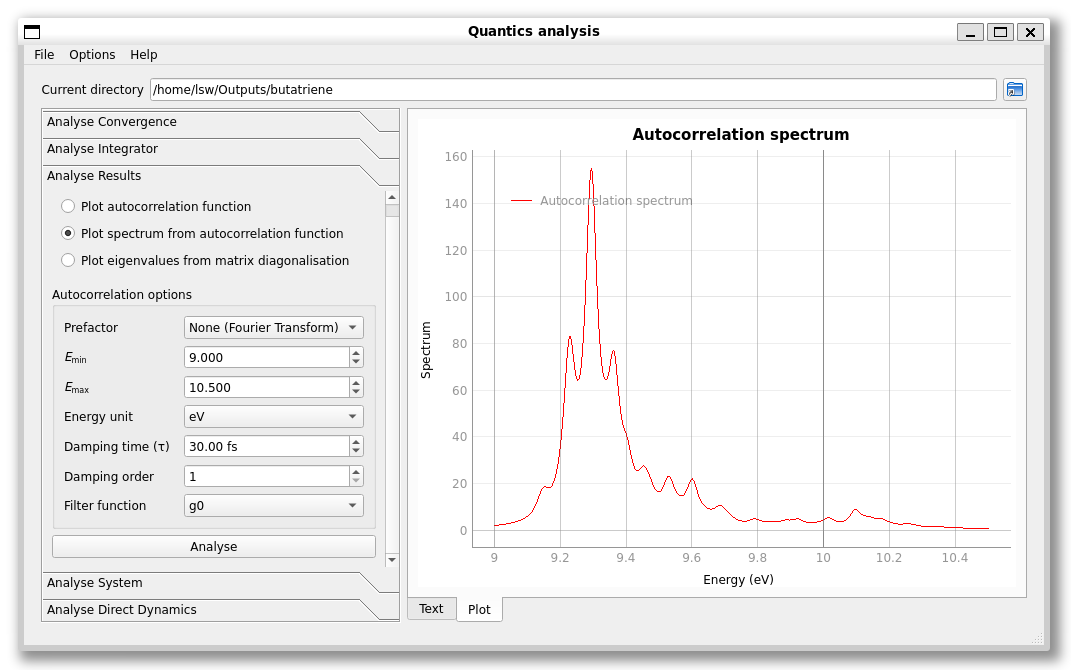
\includegraphics[width=\textwidth]{img/but_spectra_gui.png}
        \caption{Absorption spectrum from the excitation to the lower state \(S_1\) as seen in the GUI.}
        \label{fig:but_spectra_gui}
    \end{minipage}\hfill\begin{minipage}[t]{.42\textwidth}
        \centering
        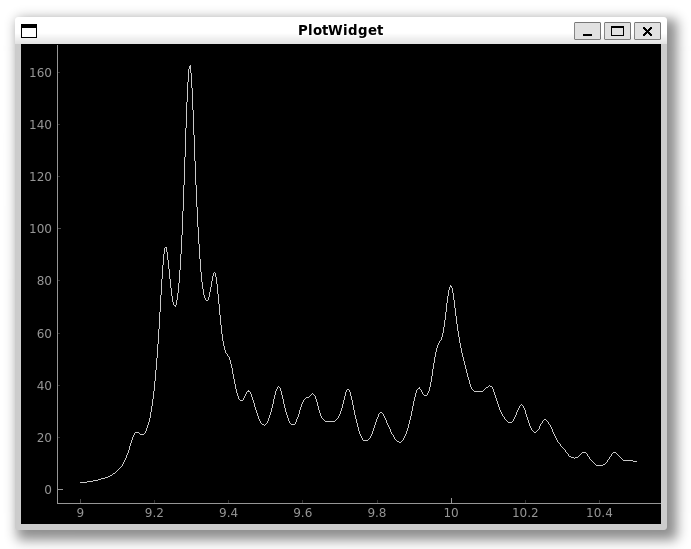
\includegraphics[width=\textwidth]{img/but_spectra_python.png}
        \caption{Combined absorption spectrum using the code in listing \ref{lst:sumspec}}
        \label{fig:but_spectra_python}
    \end{minipage}
\end{figure}

\begin{wrapfigure}{l}{0.45\textwidth}
\begin{code}\begin{minted}{python}
import numpy as np
import pyqtgraph as pg
s1 = np.load('s1.npy')
s2 = np.load('s2.npy')
x = s1[:, 0]
y = s1[:, 1] + s2[:, 1]
pg.plot(x, y)
pg.exec()
\end{minted}
\caption{Summation of spectra using NumPy arrays, then plotted using pyqtgraph.}
\label{lst:sumspec}
\end{code}
\end{wrapfigure}

Unfortunately, the combination of spectra cannot be performed inside the GUI as of yet. However, it is still possible to use the GUI to save the underlying NumPy arrays, which can then be combined. To do this, we right click on the graph and click ``Save .npy data'', then save this file with name \texttt{s1.npy} (for example) in a known directory. Navigate to the other output directory---all parameters have already been set so simply click ``Analyse'' again. Save this file with name \texttt{s2.npy} inside the same directory as \texttt{s1.npy}. These .npy files can be loaded in a Python script, summed, and plotted using listing \ref{lst:sumspec}, either by writing a Python file and executing it or calling \texttt{python3} on the command line. Alternatively, \textit{matplotlib} can be used instead of pyqtgraph for more customisable, publication-quality graphics.

Despite the limitations of the GUI in this case, hopefully it is still clear how using the GUI can be more intuitive, faster, and more convenient than the CLI. The next section, \S\ref{ssec:limitations}, details more of these limitations.

\subsection{Limitations and future work}\label{ssec:limitations}

While a substantive amount of work went into ensuring the project is complete as possible, there are many limitations to the project. Some limitations have already been discussed in the relevant implementation sections. In general, the limitations for this project can be categorised into two areas: limitations due to lack of time, and limitations due to the Fortran code. Both of these categories can be fixed with future work, and as such, this section also covers recommendations for future work in the \textit{Quantics} package.

\subsubsection{Using F2Py}

\textit{F2Py}, which is short for Fortran to Python interface generator, is a NumPy subpackage that provides a direct connection between Fortran and Python code. In particular, Fortran arrays can be directly accessed and retrieved from memory without the need to write the file to the disk by the Fortran program, then read the file from the disk by Python. This would be essentially equivalent to the ``Analysis GUI'' and ``Existing Fortran analysis programs'' merged together in Fig. \ref{fig:new_api}.

Implementing this requires knowledge of the \textit{Quantics} Fortran codebase. \textit{Quantics} is a very large project, and its GitLab repository already contains 225.1 MiB of data. If this task is to be implemented, it should be relegated to someone who already has prior experience working with Fortran and \textit{Quantics}.

However, perhaps a more suitable question is to ask whether using \textit{F2Py} would speed up the GUI significantly. While fetching the array from memory is definitely quicker than writing to disk then retrieving it, the implementation for reading floats in the \texttt{AnalysisTab} class can parse around one million floats per second, using calculations from \S\ref{sssec:read_floats} and \S\ref{ssec:unit_testing}, which is fast enough to be unnoticeable in almost all cases. The slowest part of the GUI implemented so far is probably the splitting of the 2D NumPy array to generate a 3D array in \S\ref{sssec:showd1d} (of which there may be a quicker implementation possible). As such, while the use of \textit{F2Py} would be an improvement, the gain in speed is too marginal to recommend working on.

There are other potential uses of \textit{F2Py} which are mentioned in \S\ref{sssec:input_parser}.

\subsubsection{Silent errors}\label{sssec:silent_errors}

A problem with interfacing with command line problems that had been previously mentioned in \S\ref{ssec:subprocess} is that the output of a command line program needs to be consistent such that the following code written in Python can succeed. Should this consistency fail the command line program should return a non-zero exit code. However, few of the \textit{Quantics} analysis programs written in Fortran do this, which leads to errors such as in Fig. \ref{fig:subprocess_wrong_error}, where the error produced is related to a failure in the following code rather than the actual error which preceded it.

However, there is a slightly more dangerous circumstance which occurs if there is no error raised by the following code. The situation in Fig. \ref{fig:subprocess_wrong_error} happened because a blank file was produced by the analysis program which \texttt{readFloats} failed to read. Some programs return exit code 0 on failure and do not produce any file, namely \texttt{rdgpop}. For this program, as the output's filename (\texttt{gpop.pl}) is fixed, if a \texttt{gpop.pl} already exists in the directory and \texttt{rdgpop} returns an error, the GUI will plot the file that already exists in the directory rather than show an error, which is extremely misleading. Such occurences are named \textit{silent errors}---no error popup is produced and the only way the user would know that there was an error is through inspecting the command line output in the text widget.

While there are Python implementations to fix this issue (such as checking whether a file exists beforehand, or deleting the output file after the analysis is complete), the problem can be resolved by simply ensuring a non-zero exit code is returned if there is an error with the analysis program. If the Fortran program is terminated using \mintinline{fortran}{STOP}, then simply writing a number afterwards will generate the exit code, e.g.~\mintinline{fortran}{STOP 1} will terminate the program with exit code 1.

\subsubsection{Input file parser}\label{sssec:input_parser}

While it is certainly good to catch and raise any errors and explain them to the user, it is better to prevent errors happening at all. In particular, errors that occur due to invalid parameters, such as selecting a state higher than the total number of states, or a mode index higher than the total number of modes, can be prevented if the maximum value of the spinbox is set to the number of states/modes. This can be done by overriding \texttt{optionSelected} in the analysis class and using something like \mintinline{python}{self.spinbox.setMaximum(n_state)}. However, the number of states/modes needs to be known for this to happen.

This information can be obtained from the \texttt{input} file. This has already been used for the number of GWPs in \texttt{gwptraj} (\S\ref{sssec:gwptraj}) and the mode labels in \S\ref{ssec:coordinate_selection}. However, there are hundreds of possible parameters that can be used in the \texttt{input} file, and the implementation used in \S\ref{sssec:findmodelabels} only covers a limited range of possible cases. For the rest of the cases the user has to manually input these values, which is not particularly desirable.

\begin{wrapfigure}{r}{0.5\textwidth}
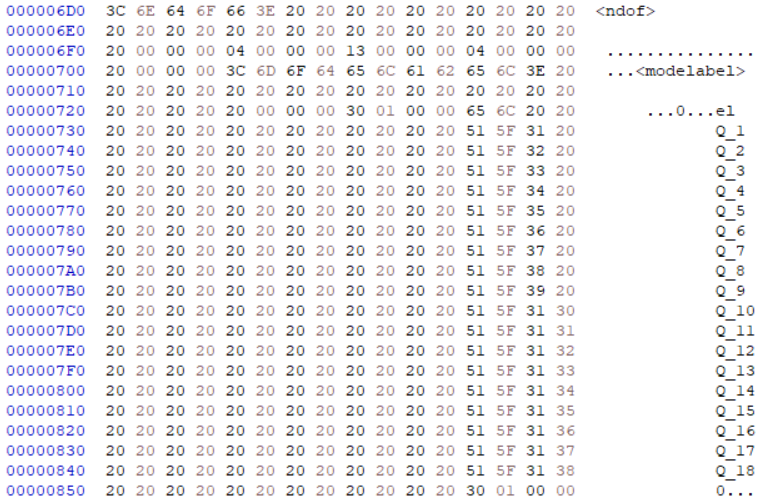
\includegraphics[width=\linewidth]{img/header_info.png} 
\caption{The number of DOFs and mode labels shown in the \texttt{dvr} header using a hex editor.}
\label{fig:header_info}
\end{wrapfigure}

An input file parser would be useful to solve these problems. It can be a class instance belonging to the main window, which is refreshed when the directory is changed by the user. Useful information can then be extracted from this instance when necessary. Technically, a parser already exists in the \textit{Quantics} package, named \texttt{mctdhinp.py}. However, it is extremely outdated (originally written in Python 2), can only extract a limited number of parameter values, and has unintuitive methods and attributes. As such it was decided the existing parser was not suitable for the GUI and manual methods to read the input file were implemented as mentioned above.

Alternatively, some relevant information are stored in the ``headers'' of some files such as \texttt{psi} and \texttt{dvr} (Fig. \ref{fig:header_info}). For Fortran programs that require these files, this is the implementation that is used to extract information such as a list of mode labels without needing to reading the input file. However, these headers are written in a binary format which is not particularly easy to extract information from. If the relevant subroutine which reads these header can be wrapped in a Python function (possibly using F2Py), this could potentially save the enormous effort of writing code that can parse the input file.

\subsubsection{\texttt{CoordinateSelector} and menu-based programs}

The \texttt{CoordinateSelector} widget as discussed in \S\ref{ssec:coordinate_selection} writes the correct input for option 20 (Listing \ref{lst:showsys_menu}, coordinate selection) in the menu-based program \texttt{showsys}. However, it should also be able to change the axis limits/bounds of \(x\) and \(y\), and provide and change the units of the DOFs. In the \texttt{showsys} menu, these options are located seperately as option 30 and 60/90, respectively. Fustratingly, changing the values for these options require the \textit{mode index} rather than the \textit{mode label}, which require the DOF to be specified as the index of the order in which the DOF is given in the \texttt{input} file, similarly to the parameter in \texttt{showd1d} (\S\ref{sssec:showd1d}).

To implement this in Python would require much more complicated code to parse the input file (also discussed in the section above). It would be potentially easier to simply combine the options together in the Fortran program, allowing specifications such as \texttt{modelabel1 x -4.0 4.0 au} and \texttt{modelabel2 0.1 au}. Even better would to have this implemented as an alternate parameter-type interface such that navigating the menus using code is not necessary at all.

\subsubsection{3D plots}

While pyqtgraph has support for 3D plots, they require an external package known as \texttt{pyopengl} which provides Python bindings to OpenGL. I could not get this working on my machine, so any 3D plots did not work and thus were not implemented. This is unfortunate as a surface plot is a particularly useful visualisation to view potential energy surfaces, such as in Fig. \ref{fig:conical_intersection}.

In addition, the pyqtgraph API for 3D plots is still relatively undeveloped (e.g.~the use of \texttt{pyqtgraph.exporters} does not function for 3D plots), and is subject to change as the pyqtgraph developers are considering using a package known as \textit{VisPy} to provide alternative OpenGL bindings\footnote{\url{https://pyqtgraph.readthedocs.io/en/pyqtgraph-0.13.3/api_reference/3dgraphics/index.html}}. Alternatively, if the use of 3D is of the utmost importance, the more mature \textit{matplotlib} package can produce a static image of a 3D plot which can be embedded in the plot widget.

\subsubsection{Other analysis programs}

As mentioned in \S\ref{ssec:summary}, all functioning analyses included in the \texttt{analysis} program were implemented in the GUI. However, there are still many other useful programs included in \textit{Quantics} that were not included in the GUI such as \texttt{showspf}, which plots the SPFs, and \texttt{adpop}, which plots the adiabatic state populations. There are far too many to be feasibly included in the timeframe of the project.

There are also programs such as \texttt{rddddb} and \texttt{ddtraj}, used for DD-vMCG simulations, that were considered as possible candidates for integration. In particular, \texttt{rddddb} produces a geometry for each entry, and \texttt{ddtraj} shows the molecular structure along a trajectory. These programs produced a \texttt{plot.db} file containing data in a \textit{Gaussian}-type format that could be read by a molecular structure viewer such as \textit{Jmol}.

However, just as we did not want to plot to open in a new window such as in \textit{gnuplot}, instead opting to plot graphs natively inside the GUI using pyqtgraph, the same would ideally go for \textit{Jmol}. However, there is no equivalent, suitable Python package that can be integrated easily in a PyQt window. A possible solution is to use the JavaScript package \textit{JSmol} and embed this in the GUI using a web browser, using a seperate package named \textit{PyQtWebEngine}. A local server can be run serving a basic webpage interfacing with \textit{JSmol}.

However, \textit{JSmol} is not as efficient as \textit{Jmol} as it mostly contains code auto-translated from Java. The \texttt{plot.db} files produced by \texttt{rddddb} and \texttt{ddtraj} methods typically contain a list of thousands of geometries which generate a large amount of latency in \textit{JSmol}. As such, the best solution at the moment is to simply open a \textit{Jmol} window, or some molecular geometry viewer that uses OpenGL is found which can be embedded in PyQt's \texttt{QOpenGLWidget}.

\subsubsection{Miscellaneous}

As with all things written in code, there may be bugs in the GUI, where the functionality does not work as expected or gives an error where there should not be. While great effort has been used to fix these bugs, there are likely many more which are not yet found, especially relating to the interface with menu-based programs, which is rather tentative. A user can report any bugs to the GitLab issues page, detailing the problematic files and the steps to reproduce them. However, as a limited number of people work on the \textit{Quantics} package this feature is rarely used.

If the keywords \texttt{time-not-fs} and \texttt{energy-not-ev} are specified in the \texttt{input} file the times and energies are given in atomic units. In this case a flag such as \texttt{-nofs} must then be given using the additional options box to correct the values. However, the units given in the labels are fixed strings in the code, and this will end up producing the wrong unit in the plot. This could be fixed by manually adding a \texttt{nofs} checkbox in the relevant parameter container, at the cost of complicating the code a little.

Analyses that read the QC database \texttt{database.sql} must currently navigate to the folder that the file is in, as typically this folder is in a different directory than the output files. It would be useful if the GUI can read the database from the output file folder without needing to navigate to a seperate directory. This can be done by reading the relevant part of the \texttt{input} file, then implementing an attribute with a getter and setter in the analysis class that refreshes when the user enters a directory. The \texttt{required\_files} dictionary can then contain this attribute instead of the default \texttt{database.sql}.

Finally, the project contained a case of ``re-inventing the wheel''. Namely, the \texttt{readFloats} function (\S\ref{sssec:read_floats}) performs an identical goal to the NumPy function \texttt{numpy.loadtxt} (or \texttt{numpy.genfromtxt} which is more customisable as it has more parameters), which was only ``discovered'' after the method had already been implemented. While the existing implementation is already very fast, one may consider replacing the current implementation with the more efficient NumPy method. Additionally, there are PyQt modules that can interface with SQL databases, namely \texttt{QtSql.QSqlDatabase}. This could potentially replace something like \texttt{querydb} (\S\ref{sssec:querydb}) but would require more work to integrate this widget into the .ui file.

\bibliography{report}

\section{Appendices}\label{sec:appendix}

\subsection{Explanation of regular expressions}\label{ssec:regex}

\subsubsection*{\S\ref{sssec:read_floats}: regex to capture floating point values}

\begin{code}\begin{minted}{text}
[+-]?                   optionally a + or - at the beginning
\d+(?:\.\d*)?           a string of digits, optionally with decimal point and 
                        possibly more digits
(?:[eE][+-]?\d+)?       optionally an exponential (e+N, e-N, EN) at the end
|                       alternative: matches either the above or below
\.\d+                   catches floats that start with decimal like
                        .25
\end{minted}
\end{code}

\subsubsection*{\S\ref{sssec:rdspeed}: regex to capture dates}

\begin{code}\begin{minted}{text}
\w{3}                   matches three characters (the month: Jan Feb Mar, etc.)
\s+                     matches one or more whitespace
\d{1,2}                 matches one or two digits (the month: up to 12)
\s+                     matches one or more whitespace
\d{2}:\d{2}:\d{2}       matches the time: two digits (hour), colon, two digits
                        (minutes), colon, two digits (seconds)
\end{minted}
\end{code}

\subsubsection*{\S\ref{sssec:ortho}: regex to capture \texttt{ortho} output}

\begin{code}\begin{minted}{text}
#.*?                    matches the header, which starts with a # symbol and any
                        number of characters after it up to the symbol below. the
                        ? means to match as little as possible ("lazy") rather 
                        than the default match as much as possible ("greedy")
\n                      matches a new line
(.*)                    only this part is captured and returned from The
                        regex. with the DOTALL flag this captures anything up to
                        the symbol below
#                       matches the first character of the header below the grid
\end{minted}
\end{code}

\subsubsection*{\S\ref{sssec:rdtiming}: regex to split \texttt{timing} file}

\begin{code}\begin{minted}{text}
(?<=Clock)\n            the re.split splits on any match the regex makes, not
                        only any groups captured with (), which has a different
                        meaning in re.split (see python documentation). to make
                        matches but not keep them we have a positive lookbehind.
                        a new line is matched (this is deleted and splits the
                        string) only if there is the text 'Clock' preceding it,
                        which is the name of the last column header
|                       alternative: matches either the above or below
\n(?=Total)             similarly, the positive lookahead means match a new line
                        only if the text 'Total' succeeds it. this is the next
                        word after the subroutine grid, as it gives the total time
                        taken
\end{minted}
\end{code}

\subsubsection*{\S\ref{sssec:findmodelabels}: regex to extract information from SPF-SECTION}

\begin{code}\begin{minted}{text}
S(?:PF-)?               match S or SPF-
BASIS-SECTION           match BASIS-SECTION
\s*\n                   match any number of whitespace after, then a new line
(.*)                    capture any sequence of characters here until the following
                        regex (with re.DOTALL flag)
\nend-s(?:pf-)?         match s or spf- after a new line
basis-section           match basis-section
                        note this regex is also run with the re.IGNORECASE flag
                        as the section start and end titles do not necessarily have
                        the given case
\end{minted}
\end{code}

\subsubsection*{\S\ref{sssec:findmodelabels}: regex to find mode labels in SPF-SECTION}

\begin{code}\begin{minted}{text}
(.+?)                   match one or more characters (lazy), including commas and
                        whitespace (this is then split by comma and have 
                        surrounding whitespace removed)
=                       match an equals sign
(?:                     match, but do not capture this part
   [ \d,]               match a space, digit, or comma
   |                    or
   id                   match the characters 'id' (special keyword)
)*                      any number of the last part
\end{minted}
\end{code}

\subsection{Input and operator files for butatriene}\label{ssec:inputop}

\subsubsection*{Input file}

\inputminted{text}{inputop/butatriene.inp}

\subsubsection*{Operator file}

\inputminted{text}{inputop/C4H4linear.op}

\end{document}